%%%%%%%%%%%%%%%%%%%%%%%%%%%%%%%%%%%%%%%%%
% Masters/Doctoral Thesis 
% LaTeX Template
% Version 1.43 (17/5/14)
%
% This template has been downloaded from:
% http://www.LaTeXTemplates.com
%
% Original authors:
% Steven Gunn 
% http://users.ecs.soton.ac.uk/srg/softwaretools/document/templates/
% and
% Sunil Patel
% http://www.sunilpatel.co.uk/thesis-template/
%
% License:
% CC BY-NC-SA 3.0 (http://creativecommons.org/licenses/by-nc-sa/3.0/)
%
% Note:
% Make sure to edit document variables in the Thesis.cls file
%
%%%%%%%%%%%%%%%%%%%%%%%%%%%%%%%%%%%%%%%%%

%----------------------------------------------------------------------------------------
%	PACKAGES AND OTHER DOCUMENT CONFIGURATIONS
%----------------------------------------------------------------------------------------

\documentclass[11pt, oneside]{Thesis} % The default font size and one-sided printing (no margin offsets)

\graphicspath{{images/}} % Specifies the directory where pictures are stored

%\usepackage[round, comma, sort&compress]{natbib} % Use the natbib reference package - read up on this to edit the reference style; if you want text (e.g. Smith et al., 2012) for the in-text references (instead of numbers), remove 'numbers' 
\hypersetup{urlcolor=blue, colorlinks=true} % Colors hyperlinks in blue - change to black if annoying

\usepackage{amsmath,amsfonts,amssymb}
\usepackage{graphicx}
\usepackage{epsfig}
\usepackage{epstopdf}

\usepackage{lineno}
\usepackage{ltablex}

\usepackage[tight,footnotesize]{subfigure}

 
\usepackage{multirow}
%\usepackage[english,algoruled,vlined]{algorithm2e}
\usepackage{algorithm}
\usepackage{algpseudocode}
\usepackage{amsmath}
%\usepackage{hyperref}
\usepackage{minitoc}
%\setcounter{secnumdepth}{1}% number \part and \chapter in book classes
\usepackage{array}
\usepackage{xparse}
\usepackage{tabularx}

\usepackage{listings}
%%Define the HATP language
%
%Author: Raphaël Lallement, raphael . lallement [at] laposte . net

\usepackage{listings}

\lstdefinelanguage{HATP}{
	keywords={define,entityType,entityAttributes,
		dynamic,static,atom,set,bool,string,number,
		true,false,NULL,new,add,in,rem,
		method,operator,projects,preconditions,effects,cost,duration,subtasks,goal,
		FORALL,EXIST,IF,SELECT,SELECTONCE,SELECTORDERED, plans},
	sensitive=true,
	comment=[l]{//},
	string=[b]{"},
	tabsize=3,
	basicstyle={\singlespacing},aboveskip={-3ex}
}

\lstalias{hatp}{HATP}
 


\title{\ttitle} % Defines the thesis title - don't touch this

\begin{document}

\frontmatter % Use roman page numbering style (i, ii, iii, iv...) for the pre-content pages

\setstretch{1.3} % Line spacing of 1.3

% Define the page headers using the FancyHdr package and set up for one-sided printing
\fancyhead{} % Clears all page headers and footers
\rhead{\thepage} % Sets the right side header to show the page number
\lhead{} % Clears the left side page header

\pagestyle{fancy} % Finally, use the "fancy" page style to implement the FancyHdr headers

\newcommand{\HRule}{\rule{\linewidth}{0.5mm}} % New command to make the lines in the title page

\theoremstyle{plain}
\newtheorem*{prop}{Assumption}

\makeatletter
\newcommand{\thickhline}{%
    \noalign {\ifnum 0=`}\fi \hrule height 1.5pt
    \futurelet \reserved@a \@xhline
}
\newcolumntype{"}{@{\hskip\tabcolsep\vrule width 1.5pt\hskip\tabcolsep}}
\makeatother


% PDF meta-data
\hypersetup{pdftitle={\ttitle}}
\hypersetup{pdfsubject=\subjectname}
\hypersetup{pdfauthor=\authornames}
\hypersetup{pdfkeywords=\keywordnames}

\linenumbers % to activate the line numbers
\renewcommand\thelinenumber{\color{red}\arabic{linenumber}}

%----------------------------------------------------------------------------------------
%	TITLE PAGE
%----------------------------------------------------------------------------------------

\begin{titlepage}
\begin{center}

\textsc{\LARGE \univname}\\[1.5cm] % University name
\textsc{\Large Doctoral Thesis}\\[0.5cm] % Thesis type

\HRule \\[0.4cm] % Horizontal line
{\huge \bfseries \ttitle}\\[0.4cm] % Thesis title
\HRule \\[1.5cm] % Horizontal line
 
\begin{minipage}{0.4\textwidth}
\begin{flushleft} \large
\emph{Author:}\\
\href{http://www.johnsmith.com}{\authornames} % Author name - remove the \href bracket to remove the link
\end{flushleft}
\end{minipage}
\begin{minipage}{0.4\textwidth}
\begin{flushright} \large
\emph{Supervisor:} \\
\href{http://www.jamessmith.com}{\supname} % Supervisor name - remove the \href bracket to remove the link  
\end{flushright}
\end{minipage}\\[3cm]
 
\large \textit{A thesis submitted in fulfilment of the requirements\\ for the degree of \degreename}\\[0.3cm] % University requirement text
\textit{in the}\\[0.4cm]
%\groupname\\\deptname\\[2cm] % Research group name and department name
 
{\large \today}\\[4cm] % Date
%\includegraphics{Logo} % University/department logo - uncomment to place it
 
\vfill
\end{center}

\end{titlepage}

%\newcommand{\todo}[1]{\textbf{\textit{\color{red} #1}}}
%\newcommand{\todo}[1]{#1}
\newcommand{\note}[1]{\textbf{\textit{\color{blue} #1}}}

%----------------------------------------------------------------------------------------
%	DECLARATION PAGE
%	Your institution may give you a different text to place here
%----------------------------------------------------------------------------------------

%\Declaration{
%
%\addtocontents{toc}{\vspace{1em}} % Add a gap in the Contents, for aesthetics

%I, \authornames, declare that this thesis titled, '\ttitle' and the work presented in it are my own. I confirm that:
%
%\begin{itemize} 
%\item[\tiny{$\blacksquare$}] This work was done wholly or mainly while in candidature for a research degree at this University.
%\item[\tiny{$\blacksquare$}] Where any part of this thesis has previously been submitted for a degree or any other qualification at this University or any other institution, this has been clearly stated.
%\item[\tiny{$\blacksquare$}] Where I have consulted the published work of others, this is always clearly attributed.
%\item[\tiny{$\blacksquare$}] Where I have quoted from the work of others, the source is always given. With the exception of such quotations, this thesis is entirely my own work.
%\item[\tiny{$\blacksquare$}] I have acknowledged all main sources of help.
%\item[\tiny{$\blacksquare$}] Where the thesis is based on work done by myself jointly with others, I have made clear exactly what was done by others and what I have contributed myself.\\
%\end{itemize}
% 
%Signed:\\
%\rule[1em]{25em}{0.5pt} % This prints a line for the signature
% 
%Date:\\
%\rule[1em]{25em}{0.5pt} % This prints a line to write the date
%}

\clearpage % Start a new page

%----------------------------------------------------------------------------------------
%	QUOTATION PAGE
%----------------------------------------------------------------------------------------

\pagestyle{empty} % No headers or footers for the following pages

%\null\vfill % Add some space to move the quote down the page a bit
%
%\textit{``Thanks to my solid academic training, today I can write hundreds of words on virtually any topic without possessing a shred of information, which is how I got a good job in journalism."}
%
%\begin{flushright}
%Dave Barry
%\end{flushright}

\vfill\vfill\vfill\vfill\vfill\vfill\null % Add some space at the bottom to position the quote just right

\clearpage % Start a new page

%----------------------------------------------------------------------------------------
%	ABSTRACT PAGE
%----------------------------------------------------------------------------------------

\addtotoc{Abstract} % Add the "Abstract" page entry to the Contents

\abstract{\addtocontents{toc}{\vspace{1em}} % Add a gap in the Contents, for aesthetics
My abstract

\paragraph{Version fran\c caise}
~\\
Mon Abstract
}

\clearpage % Start a new page

%----------------------------------------------------------------------------------------
%	ACKNOWLEDGEMENTS
%----------------------------------------------------------------------------------------

\setstretch{1.3} % Reset the line-spacing to 1.3 for body text (if it has changed)

\acknowledgements{\addtocontents{toc}{\vspace{1em}} % Add a gap in the Contents, for aesthetics

TODO\ldots
}
\clearpage % Start a new page

%----------------------------------------------------------------------------------------
%	LIST OF CONTENTS/FIGURES/TABLES PAGES
%----------------------------------------------------------------------------------------

\pagestyle{fancy} % The page style headers have been "empty" all this time, now use the "fancy" headers as defined before to bring them back


\addtocounter{tocdepth}{-4}% “delete” lowest level from TOC

\lhead{\emph{Contents}} % Set the left side page header to "Contents"
\dominitoc[d]
\setcounter{minitocdepth}{2} 
\tableofcontents % Write out the Table of Contents


\lhead{\emph{List of Figures}} % Set the left side page header to "List of Figures"
\listoffigures % Write out the List of Figures
%
\lhead{\emph{List of Tables}} % Set the left side page header to "List of Tables"
\listoftables % Write out the List of Tables


%----------------------------------------------------------------------------------------
%	ABBREVIATIONS
%----------------------------------------------------------------------------------------
%
\clearpage % Start a new page
%
\setstretch{1.5} % Set the line spacing to 1.5, this makes the following tables easier to read
%
\lhead{\emph{Abbreviations}} % Set the left side page header to "Abbreviations"
\listofsymbols{ll} % Include a list of Abbreviations (a table of two columns)
{
\textbf{MDP} & \textbf{M}arkov \textbf{D}ecision \textbf{P}rocess \\
\textbf{Acronym} & \textbf{W}hat (it) \textbf{S}tands \textbf{F}or \\
}

%----------------------------------------------------------------------------------------
%	PHYSICAL CONSTANTS/OTHER DEFINITIONS
%----------------------------------------------------------------------------------------

%\clearpage % Start a new page
%
\lhead{\emph{Definitions}} % Set the left side page header to "Physical Constants"
%
\begin{itemize}
\item Agent: a human or robot.
\item Entity: an agent, an agent's joint, or an object.
\item Joint: an agent is composed by different joints (e.g. head, hand for a human; gripper, base, for a robot).
\item Action:  a tuple $(name, preconditions, target, postconditions)$. The $name$ of an action is a unique string that identifies it. The $preconditions$ are a list of properties that must be true in order to realize the action. In our system, an action is executed on a $target$, which can be a physical object, like a cup, but also an area of the environment, like a room. The $postconditions$ are the set of properties, and their values, affected by the action's execution.
\item Fact: a statetement composed by a $pubject$, a $predicate$, and a $value$.
\end{itemize}

%----------------------------------------------------------------------------------------
%	SYMBOLS
%----------------------------------------------------------------------------------------
%
%\clearpage % Start a new page
%
%\lhead{\emph{Symbols}} % Set the left side page header to "Symbols"
%
%\listofnomenclature{lll} % Include a list of Symbols (a three column table)
%{
%$a$ & distance & m \\
%$P$ & power & W (Js$^{-1}$) \\
%% Symbol & Name & Unit \\
%
%& & \\ % Gap to separate the Roman symbols from the Greek
%
%$\omega$ & angular frequency & rads$^{-1}$ \\
%% Symbol & Name & Unit \\
%}

%----------------------------------------------------------------------------------------
%	DEDICATION
%----------------------------------------------------------------------------------------

%\setstretch{1.3} % Return the line spacing back to 1.3
%
%\pagestyle{empty} % Page style needs to be empty for this page
%
%\dedicatory{For/Dedicated to/To my\ldots} % Dedication text
%
%\addtocontents{toc}{\vspace{2em}} % Add a gap in the Contents, for aesthetics

%----------------------------------------------------------------------------------------
%	THESIS CONTENT - CHAPTERS
%----------------------------------------------------------------------------------------

\mainmatter % Begin numeric (1,2,3...) page numbering

\pagestyle{fancy} % Return the page headers back to the "fancy" style

% Include the chapters of the thesis as separate files from the Chapters folder
% Uncomment the lines as you write the chapters

\setcounter{mtc}{5}


\addtocontents{toc}{\vspace{2em}} % Add a gap in the Contents, for aesthetics


\newpage


\setcounter{mtc}{5}
% Chapter Template

\chapter{Introduction} % Main chapter title

\label{chapter-introduction} % Change X to a consecutive number; for referencing this chapter elsewhere, use \ref{ChapterX}

\lhead{Chapter . \emph{Introduction}} % Change X to a consecutive number; this is for the header on each page - perhaps a shortened title

%----------------------------------------------------------------------------------------
%	SECTION 1
%----------------------------------------------------------------------------------------

In the current days robots are starting to be introduced in our lives more and more, and we can expect that, in the next years, they will complete the transition from mechanic tools, used mostly in industries, to true partners and companions. There is an increasing interest in studying how robots should behave in environments inhabited by humans, and in some works robots have been deployed in crowded and dynamic environments, like airports and museums.

Human-Robot cooperation poses a multitude of problems. Imagine a mobile robot working in a warehouse, carrying and sorting crates in different locations. Already, we are presented with quite a complex problem, where the robot needs to have a good representation of the world (i.e. position of the crates, obstacles, layout of the warehouse), to create plans to reach the goal (which crates to move, where to bring them, which paths to follow), and to have sufficient motion and manipulation skills to achieve them. If humans are present in the environment, they should be represented and considered by the robot in its plans and actions.  Modeling humans as simple moving obstacles might not be enough if we consider issues of trust, legibility, and acceptability. The robot should respect a number of social rules in the presence of humans, like maintaining a socially acceptable distance, whenever possible, from them, and approaching them from a visible positions.

The problem becomes even more complex when robots and humans need to cooperate to solve a goal, for example by sorting together the crates, or even by sharing the load of heavy objects. To understand  how to approach this problem we can observe how humans cooperate with themselves. Psychological and philosofical research \cite{pacherie2012phenomenology} characterizes the execution of cooperative actions as 'joint actions'. Sebanz et al. \cite{sebanz2006joint} have proposed that the execution of a joint action depends on three different abilities: sharing representations, predicting actions, and integrating predicted effects of own and other's actions. These abilities can be achieved by the combination of different mechanisms:
\begin{itemize}
\item Joint Attention. The ability to direct a partner's attention, in order to create a shared representation of objects and events. Humans use a large number of social cues, like gaze direction or pointing gestures, to indicate what is currently under observation. This mechanism helps filling important gaps in the knowledge of a partner, and points to the importance of understanding what others know and perceive.
\item Action Observation: observing other partners' actions is crucial in understanding what are their goals. Studies have shown that observing a person performing an action produces a motor resonance, which increases with the observer's level of expertise in the action. Understanding what others are doing allows to predict the outcomes of their activities, and even their next movements.
\item Task Sharing: humans are able to predict, in some circumstances, what others will do  even without direct observation. A notable example is a well trained sport team, which is able to act like a single entity, coordinating seamlessly. This ability suggests that humans possess a shared representation of tasks, which include actions that should be performed by each partner of the team.
\item Action Coordination: predicting actions is not enough. Humans also need to choose a complementary action, and adjusting its parameters, like the exact moment and place where it should be performed, to partners. 
\end{itemize}

It seems that robots need to have an equivalent of these mechanism, in order to cooperate in a natural and acceptable way with humans. Is this enough to include robots in our lives? Unfortunately, we just scratched the surface of the problem. While these areas are already very complex, and not completely understood, humans possess other skills, that should be translated to robots. For example, when a robot's behavior shows a degree of intelligence, humans usually try to have a conversation with it, which can lead to frustation, or often disbelief in the actual capacities of the robot. Issues such as dialogue, representation and refinement of knowledge are very complex and will be a direct focus of this work.

The goal of this thesis is, instead, to provide a framework to allow a robot to work in social environments and execute joint actions with humans in a natural way. We built our system using psychology as an inspiration, without trying to replicate accurately human mechanism, an area of work studied in cognitive systems. 

There are still not many robotic architecture that take humans into account at all levels, from planifications to execution. We will review some examples:
\begin{itemize} 
\item \cite{trafton2013act} presents ACT-R/E, a cognitive architecture, based
on the ACT-R architecture, used for human robot interaction tasks. The
architecture aims at simulating how humans think, perceive and act in
the world. ACT-R/E has being tested in different scenarios, such as
theory of mind and hide and seek, to show its capacity of modeling
human behaviors and tought.
\item In \cite{Fong_2006} the authors present  HRI/OS, an agent-based system
that allows humans and robots to work in teams. The system is able to
produce and schedule tasks to different agents, based on their capacities,
and allows the agents to interact mostly in a parallel and independent way, with
loose coordination between them. Cooperation  mainly
takes place when one agent asks for help while
dealing with a situation. In this case the HRI/OS will
look for the best agent to help, based on their availability and capacities.

\item In \cite{clodic2009shary} the authors build SHARY, a supervision
system for human robot interaction, tested in domestic environments to
perform tasks such as serving a drink to a person. Our system is an
evolution of Shary which includes new aspects, like spatial
reasoning and modeling of joint actions.
\end{itemize}

\section{Contributions}

The main contributions of this work are the following:
\begin{itemize}
\item Building a supervision system for human robot interaction, integrating novel algorithms developed in this work with existing, components.
\item Developing a novel algorithm to infer human goals and intentions.
\item Developing a novel probabilistic planning algorithm for multiple agent.
\end{itemize}

\section{System overview}
\label{intro-system_overview}
%TODO: add urls, PR2, GAZEBO, ROS, SPENCER, GTP, Move_Base, Moveit
The supervision system was developed with the following goals:
\begin{itemize}
\item Flexibility. The system is able to work in different scenarios, environments, and different robots.
\item Extendibility. The system can be easily extendable by adding or substituting modules, to introduce different capacities, without having an impact on existing components.
\item Human-Awareness. The system supports human in all its layers. Human belief management, multi-agent planning, human-aware motion and execution, and simple forms of direct interaction are explicitly included in its components.
\end{itemize}

To achieve these goals we use the well-known ROS framework\footnote{http://www.ros.org/}, which naturally supports different robots and modules.The system has been implemented and tested in simulation, using the GAZEBO simulator\footnote{http://gazebosim.org/}, and on two different robots, the PR2 by Willow Garage\footnote{https://www.willowgarage.com/pages/pr2/overview}, and the SPENCER robot\footnote{http://www.spencer.eu/}, developed in an european research project. 

The supervision system is composed by the following layers, as shown in figure \ref{fig:intro-system_architecture}:
\begin{itemize}
\item Situation Assessment. This layer produces symbolic information, using geometrical and temporal reasoning, starting from perception data. Using Situation Assessment, the robot is able to compute information like the reachability of objects, which actions have been performed by humans, and the spatial relationships (distance, orientation, and their variations) between humans and the robot. This layer also includes a Database, which collects collects all the symbolic information produced by the system. The Database is able to represent the knowledge of different agents, as viewed by the robot. Using this feature, the robot can represent, for example, the fact that a human does not know the location of an object, or that he has wrong information about its location.
\item Goal Management. This layer manages the different goals of the robot. Goals can be directly received from exernal inputs, like a human or a terminal, or generated by the robot starting from information present in the Database. For example, after deducing that the human is looking for his glasses in the Situation Assessment Layer, the Goal Management Layer can create a goal to fetch them. 
\item Plan Production and Management. This layer is charged with producing and managing plans to achieve the current goal. The system supports multi-agent plans, and so the robot will monitor other agents' action, to check if they conform to the shared-plan, and interact with the Execution Manager layer to execute the robot's actions. Plans can be managed in three different modalities: robot leader, human leader, and equal partners. Human-Awareness is supported by adapting  production, explanation, and management of plans to the level of experience on the task of the robot's partners. Additionally, this layer supports a simple form of plan negotiation, which allows humans to express preference in the allocation of tasks.
\item Execution Management. This layer handles the execution of the robot's actions, including joint actions shared with other agents. Human safety and robustness are achieved by stopping and resuming operations  when unexpected or dangerous situations arise, like a human moving into the operative area of the robot.
\end{itemize}

 \begin{figure}[h!]
	\centering
	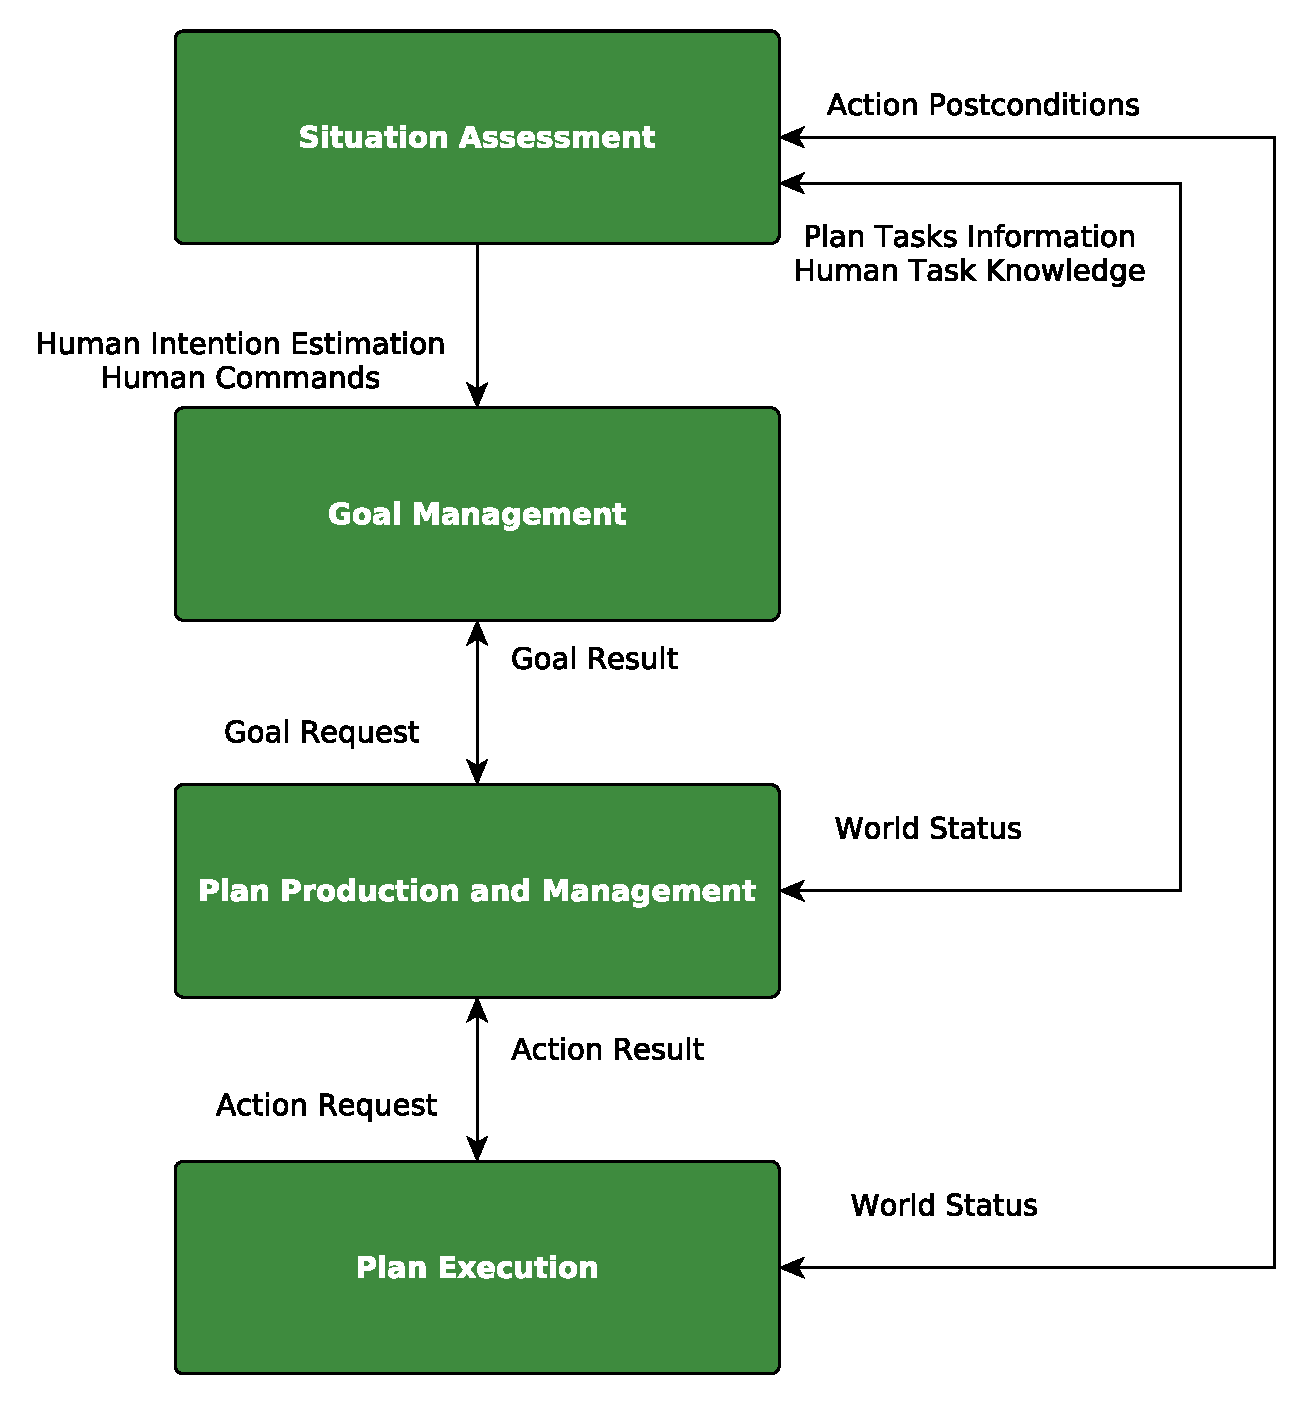
\includegraphics[scale=0.45]{img/intro/system_architecture.pdf}
	\caption[System architecture]{This picture shows the different layers of the system.}
	\label{fig:intro-system_architecture}
\end{figure}

The system also easily interface with different modules, which can be changed depending on the current needs:
\begin{itemize}
\item Task Planner. The Plan Production and Management layer provides an interface for different planners. New planners can be introduced by creating a bridge that respects the interface provided by the provided interface.
\item Motion Planners and Executors. The Execution Management layers is interfaced with a set of motion planners and an executor to accomplish the robot's movements and actions. New modules can be introduced by respecting the interface used in the layer.
\end{itemize}

\section{Organization of the Thesis}
This thesis is organized in several chapters. \ref{chapter:situation_assessment} discusses the Situation Assessment Layer, introducing its functionalities and a study to assess a part of its capacities. \ref{chapter:goal_management} shows how our system is able to receive, generate, and manage goals. \ref{chapter:plan_management} analyzes the capacity of our system to produce and manage plans. We discuss two different planners introduced in our system, and the process to explain, negotiate, and adapt plans to users. Finally, we present several plan management algorithms, with different characteristics. \ref{chapter:plan_execution} shows how our system is able to support action executed single-handedly by the robot, as well as our framework to execute joint actions with a human partner. \ref{chapter:case_study} presents two different applications where we used our system: a domestic robot helper and an airport guide. Finally, "introduce conclusion", concludes this work, discussing several possible future extensions. 

\section{Published Works}
\begin{itemize}
\item Milliez, Grégoire, et al. ``Simulating human-robot interactions for dialogue strategy learning." Simulation, Modeling, and Programming for Autonomous Robots. Springer International Publishing, 2014. 62-73.
\item Triebel, Rudolph, et al. ``SPENCER: A socially aware service robot for passenger guidance and help in busy airports.", 2015.
\item Fiore, Michelangelo, et al. ``An Adaptive and Proactive Human-Aware Robot Guide." Social Robotics. Springer International Publishing, 2015. 194-203.
\item Fiore Michelangelo, et al. ``On planning and task achievement modalities for human-robot collaboration." Experimental Robotics. Springer International Publishing, 2016.
\item Milliez, Grégoire, et al. ``Using human knowledge awareness to adapt collaborative plan generation, explanation and monitoring." The Eleventh ACM/IEEE International Conference on Human Robot Interation. IEEE Press, 2016.
\item Devin, Sandra et al. ``Some essential skills and their combination in an architecture for a cognitive and interactive" robot arXiv preprint arXiv:1603.00583, 2016
\item Caccavale, Riccardo, et al. ``Attentional Supervision of Human-Robot Collaborative Plans." The IEEE International Symposium on Robot and Human Interactive Communication (RO-MAN), 2016.
\end{itemize}
                 % Chapter Template

\chapter{Situation Assessment} % Main chapter title

\label{chap-situation_assessment} % Change X to a consecutive number; for referencing this chapter elsewhere, use \ref{ChapterX}

\lhead{Chapter . \emph{Situation Assessment}} % Change X to a consecutive number; this is for the header on each page - perhaps a shortened title

In this chapter we introduce the Situation Assessment capacities of our system. 

%TODO: Citations on Toaster. Look and add other possible citations. Cite everything. Everything!
\section{Introduction}
\label{sec:situation_assessment-intro}
\subsection{What is Situation Assessment?}
%Motivation
In any application that is not entirely composed by repetitive, precomputed, actions, robots need to possess adeguate reasoning skills, which severely depend on the quality of the representation of their environment. This representation can be more or less complex, depending on the application. Imagine, for example, a robot that needs to clean the floor of a room. For a fairly simple case, this robot would rely on a map of the room and set of lasers, or bumper sensors, to detect and obstacles. Now, imagine a household robot that needs to actively help a family that lives in an apartment, by fetching objects, providing information, and helping accomplish various tasks. Clearly, in this situation, the robot needs a deeper degree of reasoning on sensor data: laser points and camera images need to be integrated to recognize objects and humans; spatial relationships  (e.g. the cup is on the table, the human has the cup) need to be properly modeled; actions performed by humans, and their effects on the environment, need to be recognized; and so on. 

In this situation, there is a need for a process which performs different kinds of reasoning on perceptual data, and produces information that can be used by the rest of the system. This process is called situation assessment, and is deeply linked to the quality of the decisions of the robot, as explained by Endsley in \cite{endsley1995toward}. 


%what are people doing with situation assessment and belief management
Situation assessment components have been designed by different authors, but they are usually developed for specifc applications, like in \cite{Chella2010,Kluge01situationassessment}. In \cite{beetz2015robosherlock}, instead, the authors present ROBOSHERLOCK, an opersource framework that can be used to implement perception systems. Among its features, ROBOSHERLOCK supports logical queries about the world state, and so supporting task-driven situation assessment. 

\subsection{Theory of Mind}
An important part of Situation Assessment is representing other agents in the environment, not as simple obstacles, but as acting entities, with different beliefs on the state of the world, and with the capacity to affect the environment. 

Theory of Mind \cite{premack1978does} is a skill used to reason about humans' beliefs and thoughts, and how they affect actions. An ability linked to this concept is perspective taking, which is widely studied in developmental literature.  Flavell in \cite{flavell1977development} describes two levels of perspective taking: 
1) perceptual perspective taking,  the capacity to understand that other people see the world differently ~\cite{Tversky1999}; and 2) conceptual perspective taking, the capacity to attribute thoughts and feelings to other people ~\cite{Baron1985}. Studies on individuals that don't possess the required mechanisms to perform perspective taking, like young children \cite{frick2014picturing}, have put into light the difficulties these people have to accomplish everyday social relationships and confirmed the importance of this ability.

Previous works in robotics have shown that enhancing the robot's perspective taking abilities improves its reasoning capabilities, leading to more appropriate and efficient task planning and interaction strategies \cite{Trafton2005,ros2010one}. \cite{breazeal2006} showed that perspective taking can even enhance learning by imitation processes, allowing the viewer to learn a task from "flawed" demonstration, which may be correct from the teacher's point of view but are actually ambiguous. 

An important study linked to conceptual perspective taking is the 'divergent belief task'.  Formulated in~\cite{wimmer1983}, this kind of task requires the ability to recognize that others can have beliefs about the world that differ from the observable reality. ~\cite{BreazealGB09} proposed one of the first human-robot implementations, resulting in more advanced goal recognition skills. 

Not many frameworks throughly model different agent's beliefs.  Scheutz \cite{scheutz2013computational}) studied this problem, developing a computation model to represent agent's mental states. The work is oriented in particular toward communication problems and not geometrical and spatial perspective taking issues.

\subsection{Intention Recognition}
%TODO: here in particular we need something for action recognition
Another crucial skill of a robot that interacts with human is recognizing others' actions and goals. Recognizing others' goals is directly linked to modeling humans' beliefs, since, as explained by \cite{byom2013theory} "as humans, we generally believe that others act in ways that are consistent with their beliefs and goals". In psychology \cite{bruner1981} and philosophy \cite{bratman1984} literature, an intention as the wish and will to achieve a goal. Intentions memerge from contextual causes (motivations) and are present the goal is achieved or abandoned, pushing agents to undertake actions leading to that goal.

The recognition of human activities is an important topic in computer science research, which can be studied at different levels. Anticipating human actions and movements allows the robot to adapt its behavior and proactively help humans, as studied in \cite{koppula2013anticipating}. An interesting idea is using the robot's own internal models in order to recognize actions and predict user intents, as shown by the \textit{HAMMER} system in \cite{demiris2007prediction}. Sequences of actions can be linked to plans, a well-known topic called plan recognition. Several approaches have been studied in this domain using, for example, classical planning \cite{ramirez2009plan}, probabilistic \cite{bui2003general} or logic techniques \cite{singla2011abductive}.  In \cite{talamadupula2014coordination}, the authors use classical planning, with an efficient replanning strategy, in order to infer user's intentions. The system has been implemented on a PR2 robot and tested on a collaborative scenario. \cite{breazeal2009embodied} presents an architecture in which the robot is able to use its own schemas and models to infer human actions and goals, and to proactively help him achieve them. Shared plans are not explicitly represented in the system, and the robot helps the human by mapping the inferred goal information in its own beliefs, and choosing appropriate action

Two approaches that can be used for intention estimation are Interactive Partially Observed Markov Decision Processes (I-POMDP) and Inverse Learning. I-POMDP  \cite{gmytrasiewicz2004interactive} offer a rich framework that extends Partially Observed Markov Decision Processes (POMDP) in a multi-agent setting. Inference in these models can be extremely complex, but there have been attempts at solving this issue, like in \cite{doshi2009monte,hoang2013interactive}. 

Inverse Reinforcement Learning \cite{ng2000algorithms} formulates the problem of computing an unknown reward function of an agent after observing his behavior. This strategy has been applied, with Bayesian Networks (BN), in \cite{Nagai2015}, in order to learn the mental model of another agent, and choose appropriate actions for a relationship building task. A linked approach is inverted planning, which has been applied in a bayesian framework in \cite{baker2009action}  for human action understanding.

Contextual information can be used to further disambiguate complex situations. \cite{Liu2014} shows a system using BNs to understand users' intentions with an emphasis on contextual information.

It is very important to consider humans' beliefs when estimating their intentions. In a dynamic environment, agents can execute actions, modifying the state of the world without other agents being able to perceive the changes. Let us imagine a scenario. Bob comes back home from work and would like to relax while reading. He lays down on a sofa with a book, and reaches to a nearby table to grab his glasses. He does not know that his wife, during the day, moved the glasses to another room. If we would ignore Bob's beliefs on the world (i.e. he does not know that the glasses are not on the table) we could infer that, for example, Bob would like a drink while he is sitting on the sofa, or the tv remote controller. If, instead, we would know that Bob thinks his glasses are on the table (and we would use other contextual information perhaps, like Bob's habitudes) we would be able to correctly infer Bob's current intention, that is, taking his glasses, and warn him that they are not there, perhaps even fetching them for him. In robotics, an interesting framework that considers this issue is the Bayesian Theory of Mind \cite{baker2014modeling}, used to represent the inference process of an observer looking at another agent's behaviors, with POMDPs and Dynamic Bayesian Networks (DBNs).


\subsection{Dialogue}
Dialogue is a very important part of situation assessment. Agents often communicate, while executing a task together, or even when working independently, to clarify ambiguities and obtain missing information. While we will not present a specific dialogue component in this work, we have used our system in \cite{Ferreira2015}, where our belief management component and a situated dialogue system were implemented in a simulator. This model was compared with a basic system (without belief awareness) in a study with 60 interactions, in a simulated environment. We successfully showed that the dialogue management system significantly improves its efficiency, reducing the number of dialogue turns in the interaction, and its accuracy, with a higher success rate when a divergent belief situation appears.

\section{System Overview}
\label{sec:situation_assessment-overview}

In our architecture, we built a Situation Assessment layer, which is able to:
\begin{itemize}
\item  Detect and track entities.
\item  Process sensor data in order to produce symbolic information.
\item  Maintain a belief model for each agent.
\item  Infer human actions and intentions. Our system is able to perform this estimation by taking into account the current belief of humans on the world state. 
\end{itemize} 

This layer is composed by different elements, as shown in Fig. \ref{fig:situation_assessment-situation_assessment_overview}.
\begin{itemize}
\item Sensor Data. Data produced by different possible sensors (e.g. lasers, camera, etc.)
\item Entity Detection. Different components detect and track humans and objects in the environment.
\item Human Inputs. Users can communicate with the robot by using a tablet application.
\item Human Interface. User inputs from the tablet are elaborated into commands, to introduced in the Database.
\item Geometrical Reasoning. Symbolic facts are produced starting from perceptual data.
\item Belief Management. The system maintains a mental model of each agent.
\item Intention and Action Recognition. Human actions and intentions are inferred based information provided by the Geometrical Reasoning and on the belief models of the agents.
\item Database. The database stores symbolic facts produced by the system.
\end{itemize}


 \begin{figure}[h!]
	\centering
	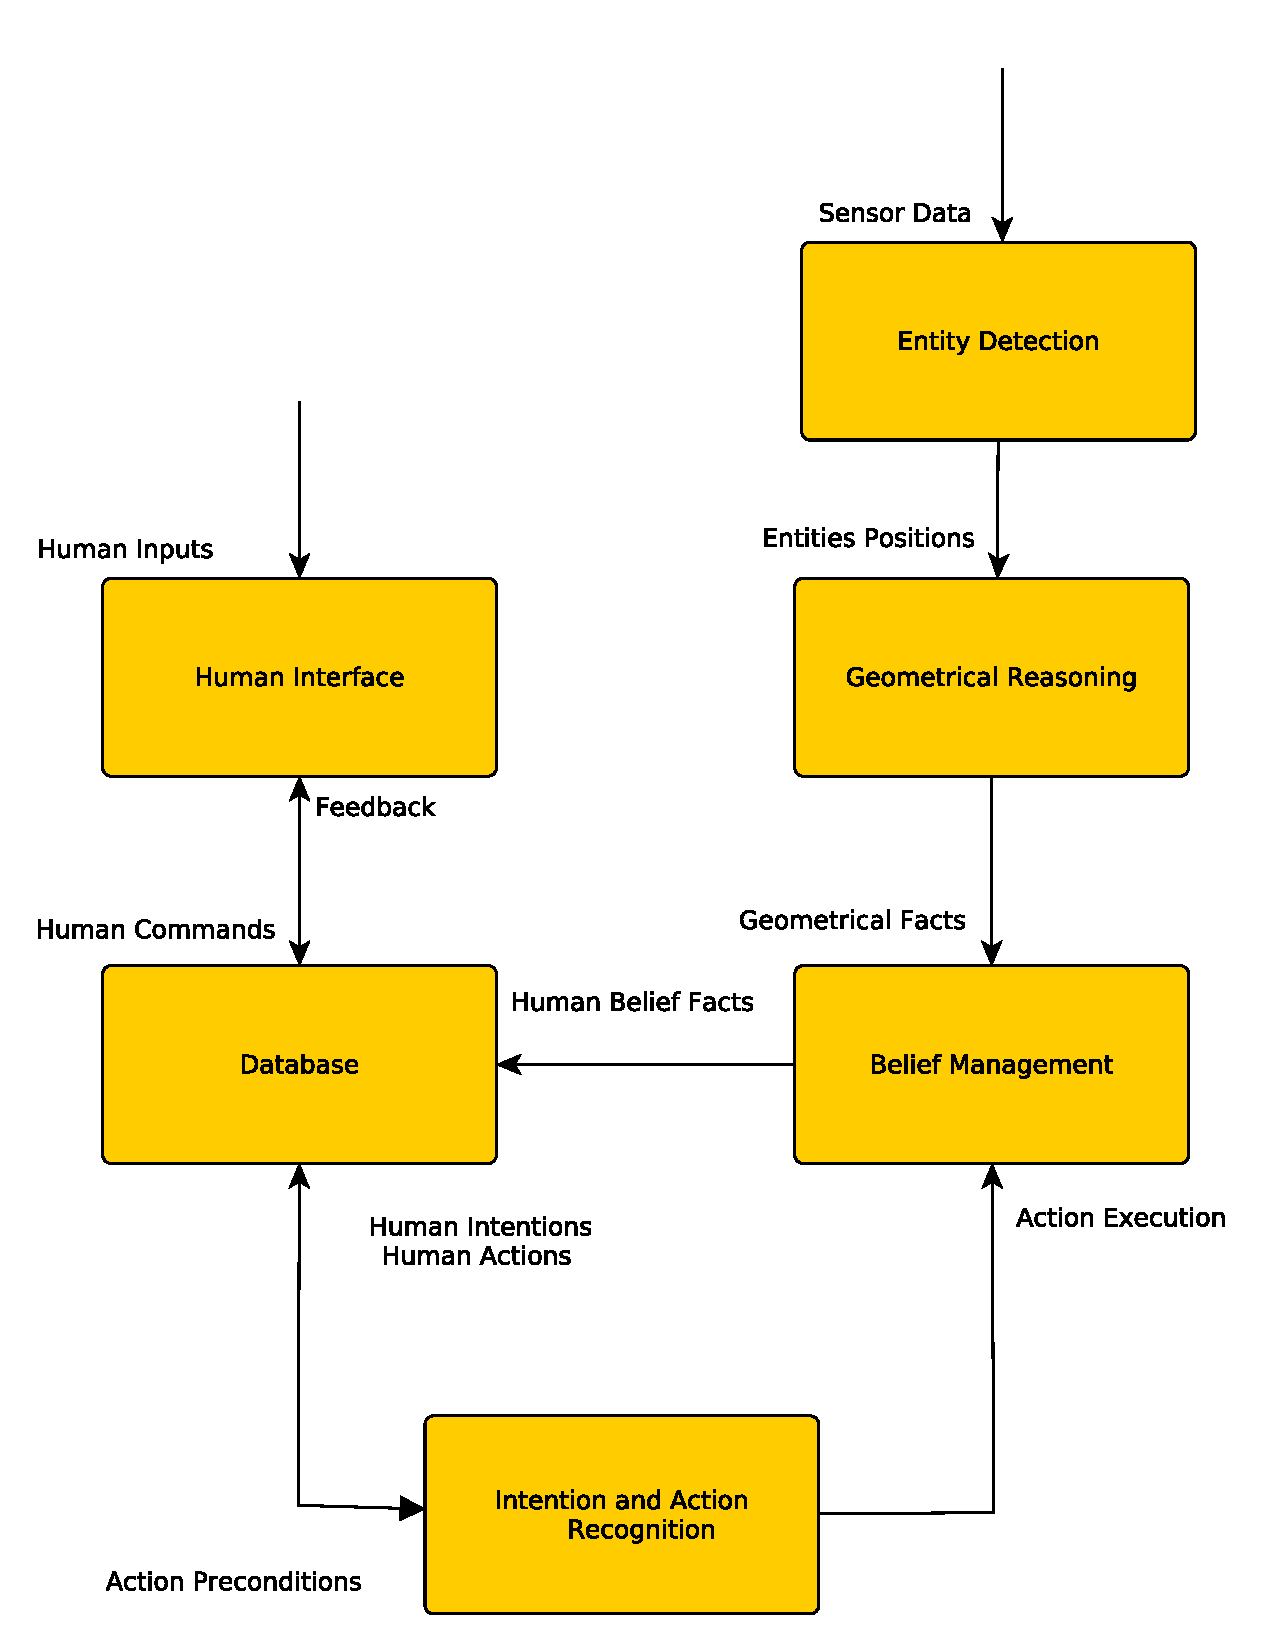
\includegraphics[scale=0.45]{img/situation_assessment/situation_assessment_overview}
	\caption{Overview of the different modules composing the Situation Assessment Layer}
	\label{fig:situation_assessment-situation_assessment_overview}
\end{figure}


In addition, the system possesses a description of the world, with a definition of all the elements known to the robot, like objects and agents, possible actions, possible intentions, intentions, etc. 
Symbolic facts are constantly produced starting from the sensor data and from the position of entities, and then the Belief Manager will update and maintain the belief model of each agent. The belief model of humans and of the robot will be used by the Intention and Action Recognition modules to infer the most likely intentions and actions performed. All these information are introduced in the Database, and can be read by other components. For example, the Goal Manager can choose a goal based on human commands or on an estimation of its intention. In a similar way, the Action Execution modules will read the Database in order to obtain the state of the world, to check action preconditions.  

Our situation assessment layer was presented in \cite{Milliez2014}, where it was used to pass the Sally and Anne test~\cite{Baron1985} on a robotic platform. The intention and action recognition capacity was introduced in \cite{devin2016some}.

\section{Object and Human Detection}
In our system, we chose to simplify perception issues, focusing on reasoning aspects. We associate a unique tag to every object that is interesting in a particular scenario.  When the robot observes a tag using a camera, it detects the corresponding object using a tag-matching algorithm.
Regarding humans, we use a motion capture software to identify and track agents moving in the environment. Using different tags, we can track the head, shoulders, and right arm of a human. Our situation assessment component has also been tested using a laser and RGB based detector in the SPENCER european project \footnote{http://www.spencer.eu/}.

\section{Human-Robot Communication}
Similarly, communication between the human and the robot is limited, in our system. Humans can give commands to the robot by using a tablet application, where they can manage the robot goals, by adding a new goal, canceling a previous one, or pausing the robot. The robot is able to provide simple verbal output by using a text-to-speech component. The robot is not able to perform real dialogues with the human but it can adapt its speech to the current tasks and scenarios, by explaining plans, informing the human if it has a problem, verbalizing its current actions, and so on. This feature will be explained fully in chapter \ref{chap-plan production and management}. 

\section{World Model and Geometrical Reasoning}
\label{sec:situation_assessment-situation_assessment}
The first step in estimating human intentions is reasoning about the environment and the belief of humans. Our world is composed by agents, the robot and humans; by objects; and by areas, which are bounded regions in the environment with semantic meaning, e.g. living room, kitchen. To be more generic, we will sometimes use the word \textit{entity} to refer to an agent, an agent's joint or an object. We can assign properties, to entities and areas to represent different information, e.g. 
an agent can be in a specific area, a box can be opened and can contain objects, a bottle can contain liquids, a mug can be hot. The $subject$ of a property is the name of the primary entity linked to it (e.g. bob, mug). 
 We divide properties in two classes: 
\begin{itemize}
\item fully observable:  can be seen by any present agent looking at the linked entity or area, e.g. the box is open
\item partially observable: can be observed by present agents only in specific situations, represented as rules linked to the object and the property, e.g. an agent can see that a box contains items only when it is open, an agent can detect that the mug is hot only when he touches it.
\end{itemize}

Using its perception abilities the robot can build a representation of the environment, starting with entities' positions. Using geometrical reasoning we can compute spatial relationships between entities, e.g. the glasses are on the shelf, the human is moving toward the library, the glasses are reachable by the human, the bottle is visible for the human. These reasonings provide a base for the perspective taking abilities of the robot. 


\section{Belief Management}
\label{sec:situation_assessment-belief_management}
In our system, agents can have divergent representations of the world. To model this aspect, the information produced by perception, geometrical reasoning and inference, are collected by the robot in \textit{belief models}, built for itself and for each agent. A \textit{belief model} is a symbolic representation of the world state, as known by an agent. In a model, the world state is represented by properties and values. To represent the lack of knowledge of an agent, the value of a property can be \textit{unknown}.

We consider our world as a dynamic environment, where properties can change and actions can be performed.  We define an action as a tuple $(name, preconditions, target, postconditions)$. The $name$ of an action is a unique string that identifies it. The $preconditions$ are a list of properties that must be true in order to realize the action. In our system, an action is executed on a $target$, which can be a physical object, like a cup, but also an area of the environment, like a room. The $postconditions$ are the set of properties, and their values, affected by the action's execution.

Since we are interested on reasoning and not perceptual aspects, we use inference, as explained in Sec. \ref{sec:situation_assessment-intention_recognition}, in order to understand when a human has performed an action. Through the predefined $postconditions$ of actions we can also infer changes in object properties, e.g. the human opens a box, so the box is now open. 

We created a rule based framework in order to build the beliefs of each agent and update them when needed. Human belief models are updated using the perspective taking skills of the robot. When the robot detects the execution of an action in the world, it updates the belief model for itself and for every human that can perceive the action, adding the action's $postconditions$ to their models. When an action is not perceived by a human (e.g. the user was in an other room), his belief model will not be updated, as he is not aware of the changes that occurred.

However, when he comes back and looks at the environment, we assign him a new belief state following a set of rules, which we will now explain. We call $H$ the agent, $HB$ his belief model, and $RB$ the robot's belief model. We also create the following predicates: $obs(p)$ means that the instance of property $p$ is observable, $valid(p,x)$ means that the instance of property $p$ doesn't contradict the current perception data of agent $x$, $value(p,m)$ is the value of predicate $p$ in belief model $m$, and $vis(p,x)$ means that agent $x$ has visibility on the linked entities of property $p$. The rules for the $valid$ predicate will be different in each property. For example the property \textit{MUG isOn TABLE} won't be valid for agent Max if he can see that there is no mug on the table. For each property $p\in HB \cup RB$:
\begin{itemize}
\item if $p \in RB, \quad p\not\in HB,\quad obs(p),\quad vis(p,H) \rightarrow value(p,HB)=value(p,RB)$.
\item if $p \not \in RB,\quad p\in HB,\quad obs(p),\quad vis(p,H) \rightarrow remove\quad $p$ \quad from \quad HB$.
\item if $p\in RB,\quad p\in HB$ then:
	\begin{itemize}
      \item if $value(p,HB)\neq value(p,RB),\\ \quad obs(p),\quad vis(p,H) \rightarrow \\ value(p,HB)=value(p,RB)$.
      \item if $value(p,HB)\neq value(p,RB),\\ \quad !obs(p),\quad !valid(p,H) \rightarrow \\ value(p,HB)=\textit{unknown}$.
	\end{itemize}
\end{itemize}
The idea of this set of rules is updating an agent's mental belief model for a property only if it's observable, or if it's not observable and perception data contradicts the current value of the property (e.g. the mug was moved from the table to the kitchen while the agent was in another room: while the agent can not see where is the mug, he can see it is no longer on the table).



\section{Action and Intention Inference}
\label{sec:situation_assessment-intention_recognition}

In order to infer human intentions, we will provide the following information to the robot: a list of known contexts, a list of known intentions, a list of known actions, a set of observations of human actions, and a belief model of humans and of itself.

We propose, as central model used for intention estimation, a framework based on BNs. We call our implementation of BN an Intention Graph (IG).
An IG is linked to a specific agent, and composed by the following layers of nodes:
\begin{itemize}
\item Context Nodes: these nodes represent contextual information, modeled as boolean variables (e.g. HotDay, ColdDay).
\item Intention Nodes: these boolean nodes represent the set of possible intentions. Each intention can conditionally depend on several contexts.
\item Action Nodes. This is the set of human actions whose preconditions . Each of these nodes is conditionally dependent on all the intention nodes. 
\item Observation Nodes. We associate to each action a different set of observation nodes, that depend conditionally on the associated action node. 
\end{itemize}

In a typical usage, the robot will create, for each monitored human, an IG, formed by the Context and Intention Nodes, which we consider statically known by the robot, and a variable list of Action and Observation nodes, which depends on the human's belief model. The robot will create action nodes for each known action whose $preconditions$ are satisfied in the human's belief model, and their related Observation Nodes. These IGs will need to be updated every time that an agent performs an action, switching the previous Action and Observation nodes with new ones, that will depend on the state of the world after the action was performed.

When monitoring a human, we set Context Nodes and Observation Nodes as \textit{evidence}, considering them observable by the robot. These information will allow us to have a good estimation of the most likely actions and intentions of the human, as explained in \ref{intention and action inference}.

An example of IG, taken from an experiment, can be seen in figure \ref{fig:situation_assessment-intention_graph}. In the following paragraphs, we will explain the role of these layers of nodes, and how the conditional dependencies between them are computed.

 \begin{figure}[h!]
	\centering
	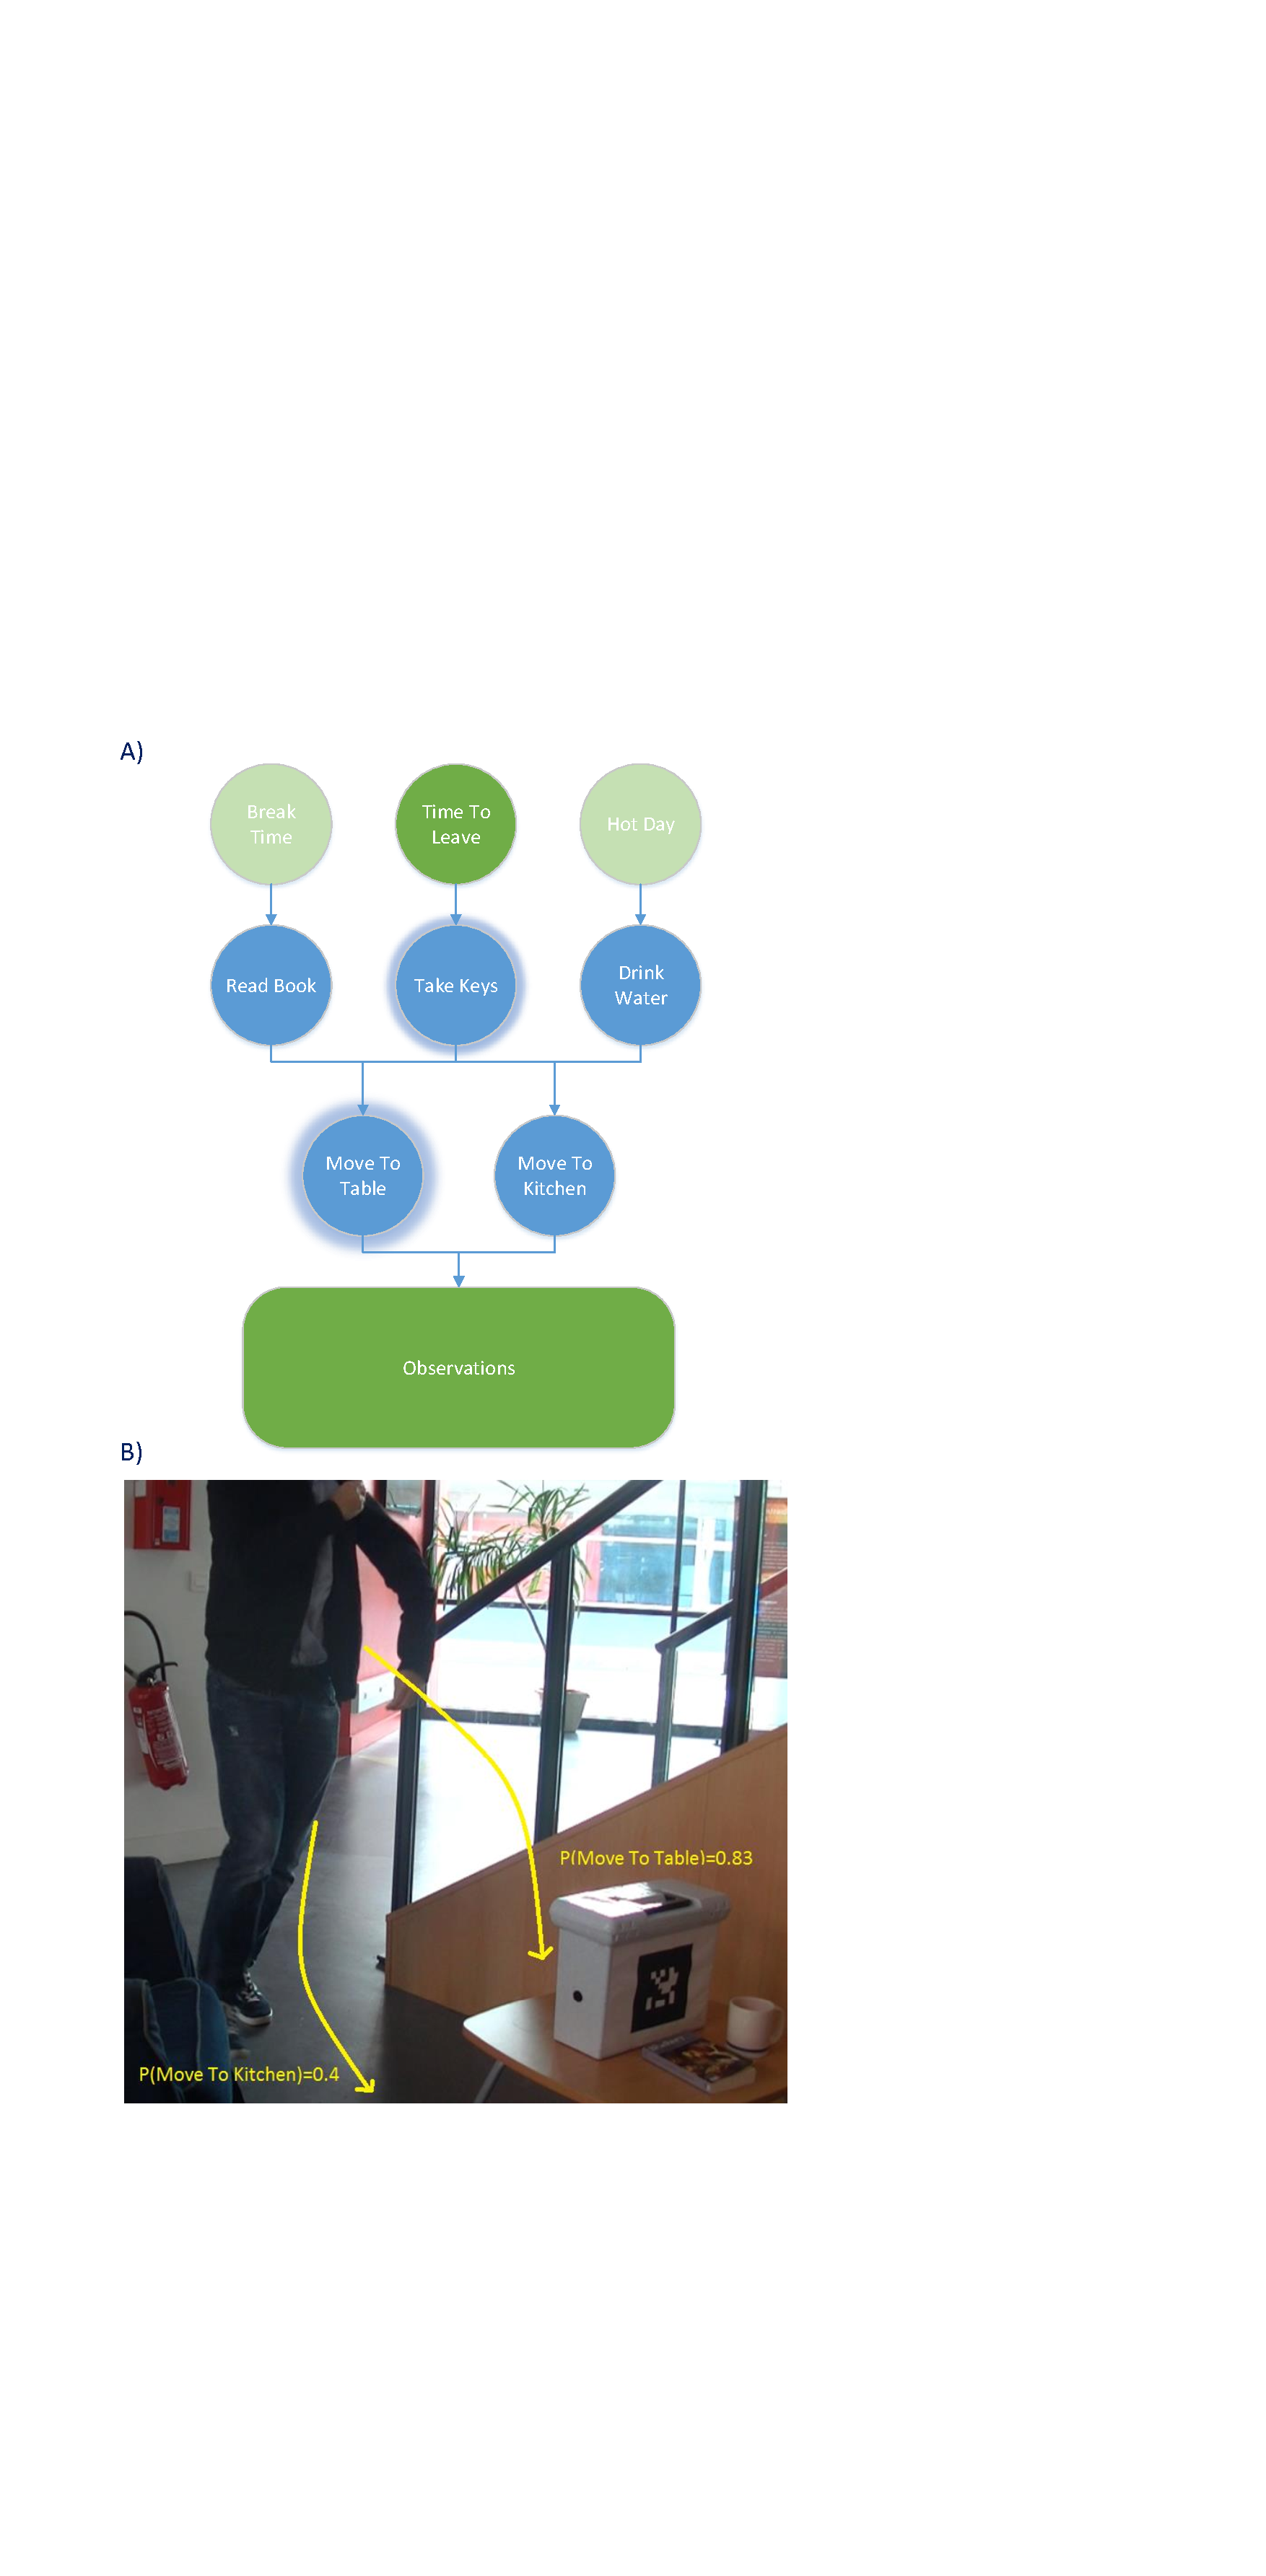
\includegraphics[trim={2cm 11cm 11cm 17cm},clip,scale=0.45]{img/situation_assessment/cookieScenario.pdf}
	\caption{A scene from our experiment. The yellow arrows show possible actions and their associated probabilities. The diagram represents the current IG. Green circles represent evidence nodes and blue circles other nodes. For the Context Nodes (top of the graph), we represented nodes with a false value as greyed out, and nodes with a true value as green. The most likely nodes in the graph are represented with a glowing effect. The observation nodes where compressed in a single block to simplify the diagram}
	\label{fig:situation_assessment-intention_graph}
\end{figure}

\subsection{From Contexts to Intentions}
We introduce a set of contexts in our domain. We consider as context any information that can be used to characterize and motivate an intention \cite{abowd1999towards}. We model a context  as a property, which can assume different values and influences the probability of a user having a particular intention. For example, we imagine that a human is more likely to be cooking at dinner time, or to drink a hot mug of tea on a cold day.

Contextual nodes can directly influence one or more Intention nodes. In this work, we chose to learn these conditional dependencies from humans, as explained in section \ref{situation_assessment-experiments}.

\subsection{From Intentions to Actions}
\label{sec:situation_assessment-action_evaluation}
To understand how actions are linked to intentions the robot needs to answer the following question: what actions would a human take, in this situation, given his belief of the world, in order to achieve its intention?
Our idea is based on the principle of rationality \cite{Dennet1989}, which states that agents tend to choose the most efficient actions, taking into account their beliefs about the world, in order to achieve their desires.

In \cite{Blakemore2001}, the authors explain that "the attribution of intentions to actions might rely on simulating the observed action and mapping it into representations of our own intention". We represent this idea by providing the robot with a set of planning models. Each one of these planning models is related to an intention, and represents all the known plans to achieve its linked goal. In this way, we can estimate how much the current human actions are compatible with the plans related to an intention.

In our implementation, for each intention known by the robot, we will create an associated Markov Decision Process (MDP), to represent all the possible plans associated to this intention. After solving the set of MDPs we will use the calculated action value function \(Q(s,a)\), to create conditional dependencies between Intention and Action nodes in the IG. Let's start by defining \(P(a|I_i=1)\), the probability that action $a$ will be performed if intention $I_i$ is true. We model this probability as \(P(a|I_i=1)=\frac{Q_i(s,a)}{\sum_b(Q_i(s,b))}\), where we normalize the value function $Q_i(s,a)$ for intention $i$ and action $a$ in the human's belief state $s$, over the value function $Q_i(s,b)$ calculated on all the monitored actions $b$. We can extend this calculation to the case where a generic number of intentions are true to compute the probabilities of action nodes: \(P(a|I_1,I_2,...,I_m)=\frac{\sum_{i:I_i=1}Q_i(s,a)}{\sum_b\sum_{i:I_i=1}Q_i(s,b)}\).

The key idea in this problem is to use the human's belief state as input for the MDPs' value functions. In this way we are using perspective taking at a planning level as the human action is consistent with his intention in his own belief state but may be irrelevant in the real world (e.g. in case of wrong belief).

Our idea is similar to \cite{karami2010human}, where human intentions are estimated using a POMDP and a set of MDPs, that simulate human policies related to different intentions. In this work we use a BN instead of a POMDP, which allows us to separate the mechanisms used for inference and for the robot's actions. Also, we improve the recognition process by including the belief state of the human.

\subsection{From Actions to Observations}
Intentions will be inferred from human actions, so the robot needs to monitor their execution. For each Action Node we define a set of four Observations Nodes: the distance of the human's body from the action's $target$, its variation, the distance of the human's hand from the action's $target$, and its variation. The conditional dependencies of the Observation Nodes are precomputed.

\subsection{Intention and Action Inference}
\label{sec:situation_assessment-intention and action inference}
We assume, in this work, that at each moment a human can only execute a single action, and the robot will react only on his most likely intention. The most likely action and intention are inferred from the BN in the following way. We call $P(n)$ the inferred probability of a node $n$, $B(n)$ the set of brothers of $n$ (that is, nodes on the same layer), and $\delta_1$, $\delta_2$ two thresholds. The robot infers that an action has been realized, or that a human has an intention following these rules: 
\begin{itemize}
\item  \(P(n_i)>\delta_1\) 
\item  \(\forall b \in B(n_i): P(n_i)>P(b)+\delta_2\), where $n_i$ is the node associated to the interested intention or action.
\end{itemize}

When the robot infers that an action has been performed, it updates the world state with its $postconditions$, triggering an update on the beliefs of all present agents. The current human intention is recorded in the Database, in order to be used by the Goal Manager.


\section{Experiments and Discussion}
\label{sec:situation_assessment-experiments}
\subsection{Case Study}
Evaluating the capacity of the system to estimate human intentions is not easy, since intentions are not directly observable. A possible solution, as shown in \cite{baker2014modeling}, is comparing the estimation of human intentions, performed by other humans, with the predictions of our system. In order to perform this comparison we created a user study where we showed participants several videos, asking them to estimate the likelihood of a set of intentions for each video, and collected their results. 

We performed an equivalence test, comparing users' intentions predictions with those of the robot, following the two one-sided tests (TOST) approach. We choose as a threshold for equivalence the standard deviation $\sigma$ of the users' answers. The idea behind this choice is that, if the robot's answers are closer than a standard deviation to the average human answers, its predictions are comparable to an average human answer from our user group. 

We defined our hypothesis as follow: 
\begin{itemize}
\item $H_0$: $\mu_{hi}-\mu_{ri}\leq-\sigma_{hi}$ OR $\mu_{hi}-\mu_{ri}\geq\sigma_{hi}$ 
\item $H_A$: $-\sigma_{hi}<\mu_{hi}-\mu_{ri}<\sigma_{hi}$  
\end{itemize}
where $\mu_{hi}$ and $\mu_{ri}$ are the human average and the robot's answer for test $i$, $\sigma_{hi}$ is the variance of the human answers for test $i$.

We performed tests to evaluate: a) prediction in absence of clues, b) prediction in the presence of contextual clues, c) prediction in the presence of belief state clues.

We built a household environment with a fixed set of furniture: a \textit{Kitchen Shelf}, a \textit{Table}, a \textit{Sofa}, and a \textit{Chair}. In this environment, we created two scenarios, composed by several tests, with two agents, \textit{Max} and \textit{Bob}, performing different actions. Each scenario contained a set of objects, and a constrained set of intentions. For the tests related to belief states, we start by showing the users and the robot a specific sequence of events, allowing them to build a mental model of the agents. We will describe in details the two scenarios and the relative tests.

\subsubsection{Cookie Scenario}
\begin{itemize}
\item Objects: a \textit{Cookie Box}, a \textit{Mug}, and a \textit{Bottle of Water} were placed on the \textit{Table}, close to each other. A pack of \textit{Cookies} was placed on the \textit{Kitchen Shelf}. The \textit{Cookie Box} could contain, or not, \textit{Cookies}.
\item Intentions: \textit{Eating a Cookie}, \textit{Drinking Water}, \textit{Reading the Book}.
\item Tests:
\begin{itemize}
	\item \textit{No Clues}: \textit{Max} approaches the \textit{Table}.
    \item \textit{Contextual Clues}: \textit{Max} approaches the \textit{Table} commenting on the warmth of the day.
	\item \textit{Divergent Belief Max}: \textit{Max} approaches the \textit{Table}.
	\item \textit{Divergent Belief Bob}: \textit{Bob} approaches the \textit{Table}.
\end{itemize}
\item  \textit{Divergent Belief Event}:  \textit{Max} and \textit{Bob} are chatting on the \textit{Sofa}. Max eats the last \textit{Cookie} from the \textit{Cookie Box} before closing it and leaving. While \textit{Max} is away, \textit{Bob} takes \textit{Cookies} from the \textit{Kitchen Shelf}, fills the \textit{Cookie Box} with them, and closes it, before leaving.
\end{itemize}

The \textit{Divergent Belief Event} was shown to the users and the robot between the \textit{Contextual Clues} and the \textit{Divergent Belief Max} events. 

We deliberately included an intention, \textit{Reading the Book}, without placing a book in the visible environment, introducing a confusing element in the scenario.

\subsubsection{Keys Scenario}
\begin{itemize}
\item Objects: A \textit{Box} was placed on the \textit{Table}, that partially occluded the sight of people approaching. A \textit{Book} and a \textit{Mug} where placed behind the \textit{Box}, so that they could be seen from the sofa but not from approaching people.
\item Intentions: \textit{Taking the Mug}, \textit{Taking the Keys}, \textit{Reading the Book}.
\item Tests and Events:
\begin{itemize}
\item \textit{No Clues}: \textit{Max} approaches the \textit{Table}.
\item\textit{Contextual Clues}: \textit{Max} approaches the \textit{Table} in a hurry, while putting on a coat.
\item \textit{Divergent Belief Max}: \textit{Max} approaches the \textit{Table} in a hurry, while putting on a coat.
\end{itemize}
\item \textit{Divergent Belief Event}: \textit{Max} is sitting on the \textit{Table}, drinking from the \textit{Mug}, while having the \textit{Keys} in his hands. His phone rings, so he drops the \textit{Keys} and the \textit{Mug} on the \textit{Table}, behind the \textit{Box}, and leaves the room. While \textit{Max} is away, \textit{Bob} comes and sits on the \textit{Sofa}, reading a \textit{Book}. When he sees the \textit{Keys}, he takes them, places the \textit{Book} on the \textit{Table}, and leaves.
\end{itemize}

The \textit{Divergent Belief Event} was shown to the users and the robot between \textit{Contextual Clues} and the \textit{Divegent Belief Max} events.

\subsection{User Study}
We built an online user study, where we presented videos related to the tests and events of the two scenarios to users, who had to evaluate the likelihood of each intentions of the scenario
on a five-level Likert scale. The user study was conducted in three languages, with users living in two different countries\footnote{A version of this user study was provided at http://goo.gl/forms/YiuFHnF63c}. We collected answers from 78 adults, performed an average, and converted them to percentile scores, in order to compare them with the robot's predictions.

Looking at users' answers (Fig. \ref{fig:situation_assessment-user_study_results}), we can see that, in the absence of clues, people rated similarly the two intentions related to visible objects. Contextual clues had the highest influence on users' ratings. This is particularly visible in the \textit{Contextual Clues} test of the \textit{Keys Scenario}, where users chose as the most likely intention \textit{Take Keys}, even if no keys were visible in the video. Divergent beliefs also influenced users decisions, but not as strongly as context. The strongest responses, over all, where given by the \textit{Divergent Belief Max} test on \textit{Keys Scenario}, which uses both divergent belief and contextual information.

\subsection{Robot implementation}
At the start of a scenario the robot scanned the environment, building a model of its world state. With our perception capacities, we can't detect if the cookie box is full or empty, and so we consider it as full at the start of a test, and update its value using the $postconditions$ of inferred human actions. We consider the box as empty when we infer that a human has taken a cookie from inside, and as full when we infer that a human has put a cookie in it.

We built different IGs for the scenarios. Each test had a different graph, related to it's main agent. We considered three different Context Nodes for these IGs: Hot Day, true when the day is particularly warm; Break Time, true when the agents are taking a pause; Time to Leave, true when it's late in the day, and the humans usually leave work and return home.

As previously said, we chose to follow \cite{Liu2014} in order to learn the link between Contexts and Intentions. We created a second user study with 15 users, in which we presented a set of 5 scenarios, each one related to one of the intentions of our tests. For each scenario we asked the users to rate the perceived link, on a five-level Likert scale, between the intention and our three contexts. We averaged users' answers and calculated the conditional probabilities between context nodes and intention nodes from these averages.


In the \textit{Cookie Scenario} the graph for the tests is constructed from the following nodes:
\begin{itemize}
\item Context Nodes: \textit{Hot Day}, \textit{Break Time}, \textit{Time to Leave}
\item Intention Nodes: \textit{Fill Cookie Box}, \textit{Eat Cookie}, \textit{Drink Water}, \textit{Read Book}.
\item Action Nodes: \textit{Move to Table}, \textit{Move to Kitchen}.
\item Observation Nodes: distance of the agent body and hand to each action's associated \textit{interesting points}.
\end{itemize}

We introduce the \textit{Fill Cookie Box} intention, not present in the human test, to allow the robot to detect when Bob fills the \textit{Cookie Box} during the \textit{Divergent Belief Event}.

Our robot doesn't have speech recognition capacities. We simulated this capacities, and set Context Nodes to plausible values, that could be extracted by watching the videos. For the \textit{Contextual Clues} test, we set the value of \textit{Hot Day} to true (since Max is commenting about the temperature), and \textit{Break Time}, and \textit{Time to Leave} to false (since no data in the video points to one of these contexts being true. Max and Bob seem to have taken a break from work before the other events are shown, in the Divergent Belief Event).
%Our robot doesn't have speech recognition capacities. and for \textit{Contextual Clues} test, set the value of \textit{Hot Day} to \textit{true}, and the value of \textit{Break Time} to \textit{false}, i.e. the robot knows that it is not the usual time for the agents to take a break.

\textit{Divergent Belief Event}, \textit{Divergent Belief Max}, and \textit{Divergent Belief Bob} were showed sequentially to the robot, which updated the agents' mental models and created new IGs accordingly. During the \textit{Divergent Belief Event} several IGs need to be created with different action and observation nodes, to follow the sequence of actions by the two agents. For example, when \textit{Max} leaves the room, \textit{Bob} has the possibility to execute the actions \textit{Take Mug}, \textit{Take Water Bottle}, \textit{Open Cookie Box}, \textit{Move to Kitchen Shelf} or \textit{Leave Room}. Intention and Context nodes remains the same in all the IGs of the scenario.


The \textit{Keys Scenario} has a similar IG, with the following differences.
\begin{itemize}
\item Context Nodes: \textit{Hot Day}, \textit{Break Time} and \textit{Time to Leave}.
\item Intention Nodes: \textit{Drink Water}, \textit{Take Keys}, \textit{Read Book}.
\end{itemize}

Action Nodes and Observation Nodes are the same as the previous scenario, and follow the same ideas during the \textit{Divergent Belief Event}. An example of IG used in the tests can be seen in Fig. \ref{fig:situation_assessment-intention_graph}. For the \textit{Contextual Clues} and \textit{Divergent Belief} test, we set the \textit{Time to Leave} context value to \textit{true} (since Max is putting a coat and seems in a hurry), and other context node values to \textit{false}. Using the component described in the previous sections, and these IGs the robot was able to obtain predictions from the user actions.

\subsection{Discussion}
\label{sec:discussion}
We performed TOST tests for each intention in the scenarios, comparing the humans' answers with the robot's, for a total of 21 tests.

We calculated p-values and performed our tests using a significance value $\alpha=0.05$.

Analyzing the results of our equivalence tests, shown in Fig. \ref{fig:situation_assessment-user_study_results}, produces some interesting information. 1) The behavior of our system is often close to human capacities. 19 tests out of 21 passed our requirements for significance level, often with very low p-value scores. 2) Context and Divergent Belief are necessary. A system without these skills would only have been able to model properly the \textit{No Clues} cases. 3) There are still some missing aspects in our system. We failed to reject the null hypothesis for two tests. In \textit{Divergent Belief Bob} users rated higher the \textit{Eat Cookie} intention than the \textit{Drink Water} intention, possibly because they thought that since \textit{Bob} filled the \textit{Cookie Box} he may want to eat a \textit{Cookie}. This makes us think that humans use deep temporal reasoning to evaluate intentions, considering the whole history of actions performed by agents.  

 \begin{figure}[h!]
	\centering
	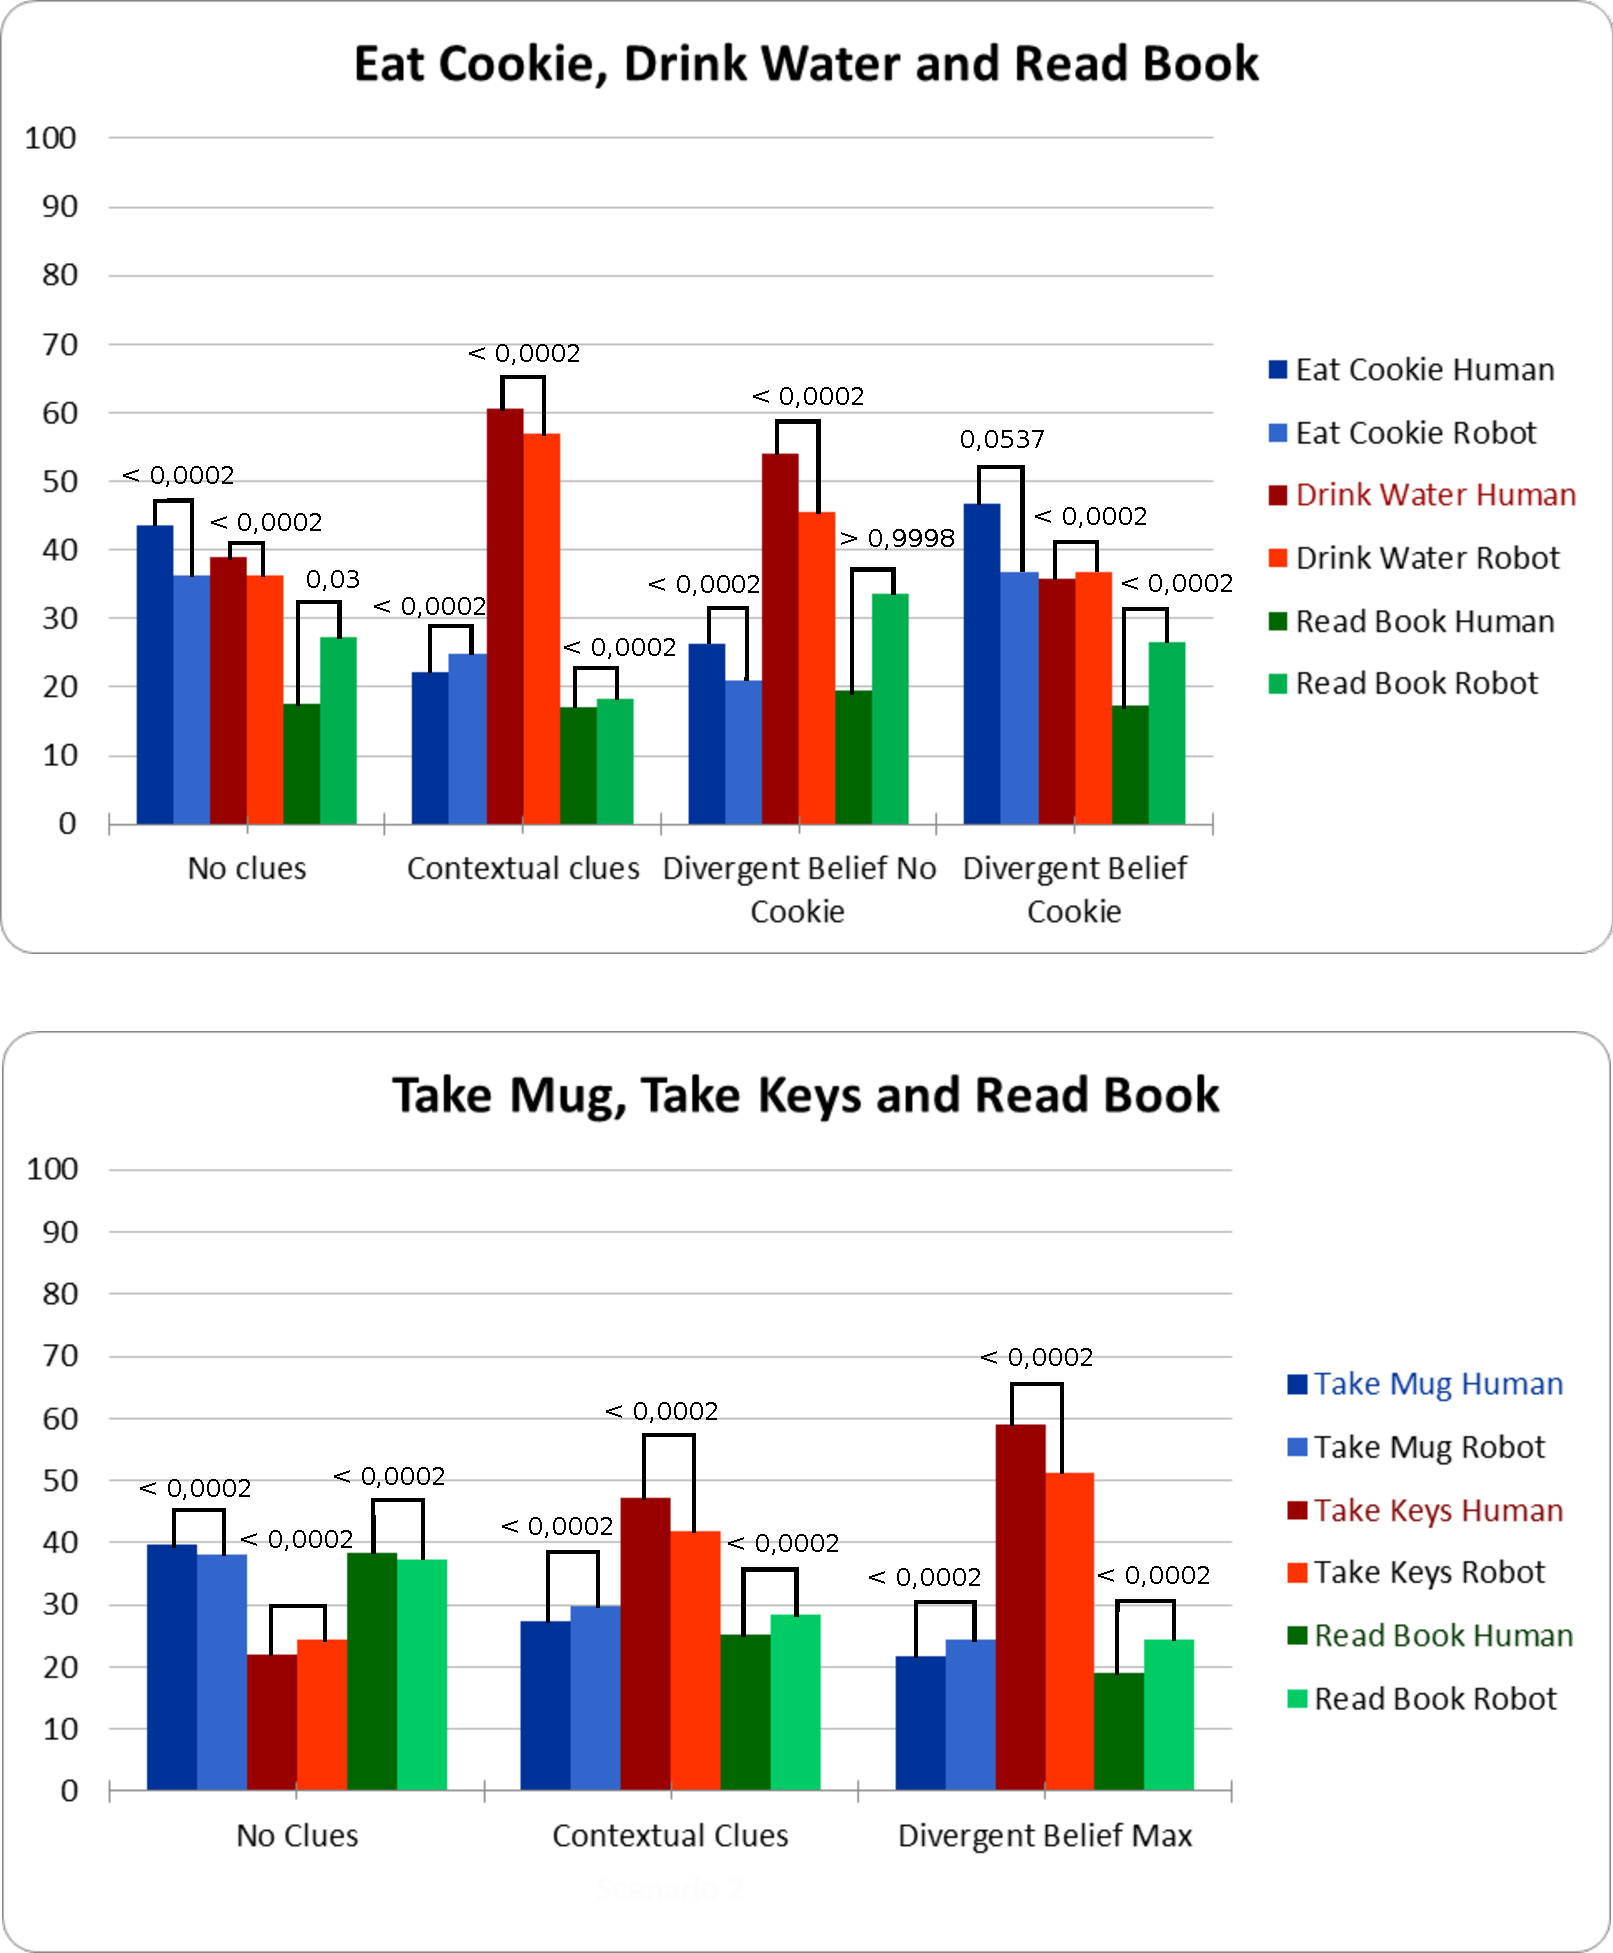
\includegraphics[clip,scale=0.32]{img/situation_assessment/pvalues1.pdf}
	\caption{Experiment results. Results from the two scenarios are represented as graphs. Intentions, as estimated by the humans and the robot, are represented by different colors, as shown in the legend of the graphs, with estimations of the same intention by the robot or the human placed in adjacent position. Each column represents the likelihood of an intention, expressed as a percentile score. P-values from the equivalence tests are shown, linking the estimation of an intention by the humans and by the robot.}
	\label{fig:situation_assessment-user_study_results}
\end{figure}




% Chapter Template

\chapter{Goal Management} % Main chapter title

\label{chapter:goal_management} % Change X to a consecutive number; for referencing this chapter elsewhere, use \ref{ChapterX}

\lhead{Chapter . \emph{Goal Management}} % Change X to a consecutive number; this is for the header on each page - perhaps a shortened title
In this Chapter we introduce the goal management characteristics of our system. Section \ref{sec:goal_management-intro} introduces the important topic of goal generation and management. Section \ref{sec:goal_management-overview} shows the main characteristics of this layer. Finally, section \ref{sec:goal_management-choosing} discusses our implementation in details.

\section{Introduction}
\label{sec:goal_management-intro}
An essential characteristic of an intelligent robot is acting with goal-oriented behaviors. Managing and generating goals has not been a primary focus of the AI community and, to our knowledge, there are not many works that deal with this important, and complex, subject. 

Let us imagine, for example, an household robot, helping a family to accomplish a number of tasks. At each moment, this robot can have several different goals, which could pre-programmed, requested by users, or selected by the robot by reasoning on the state of the world. New goals could even arise while the robot is already acting. What should the robot do in these situations? Should it abandon the current task and start executing a more important goal? Or perhaps, if the current task is almost accomplished, should it finish executing it?  

It's clear that managing goals is a hard problem, involving issues such as scheduling and risk analysis. An example of work that studies this problem is \cite{hanheide2010framework}, where the authors present a framework to generate and manage goals in a robotic system. Goals are created, based on the system's state, from a number of generators and encoded in terms of importance and urgency. The framework has been used in a robotic explorer architecture.

\section{Overview}
\label{sec:goal_management-overview}
While goal management is not a focus in this work, we introduce a simple system that allows the robot to select which goal to activate from a list of possible goals. This layer is able to:

\begin{itemize}
\item Generate new goals by reasoning on the current state of the world.
\item Select the next goal to achieve by analyzing the importance of each possible goal.
\item Activate other layers of the system to achieve goals.
\item Managing goals by pausing the current goal, aborting it, switch from one goal to another, etc.
\end{itemize}


We do not include mechanisms for scheduling or to evaluate the length of time to achieve a goal, which would improve the quality of choices performed by our system.

\section{Generating and Choosing Goals}
\label{sec:goal_management-choosing}
This layer has a list of possible goals that can be achieved by the robot, which may differ from the list of intentions introduced in section \ref{sec:situation_assessment-intention_recognition}, since some goals could be achieved only by humans or only by the robot. At each moment, the layer also has a list of instantiated goals, that need to be managed.

Each goal is represented by a tuple $(name, parameters, activation, priority, status$), where $name$ is a unique string identifying the goal, $parameters$ is a set of variables related to a specific instance of a goal, $activation$ is a set of properties used to generate an instance of the goal, and $priority$ is a string that can assume the possible values $(low, medium, high)$ and represents the importance of the goal. The priority of a task is precomputed, or can be selected by the human when requesting a task. At each moment a goal instance has a $status$, which can be $active$, meaning that the robot is executing actions to achieve it; $ready$, meaning that the goal can be selected to become $active$; $paused$, meaning that the goal was $active$ but has been temporarily abandoned to pursue another goal; $aborted$, meaning this instance of the goal can be erased; or $completed$, meaning that the goals has been achieved.  

At the start of the system, there are no active goals. Goals can be instantiated, starting with a $ready$ status, in different ways:
\begin{itemize}
\item The $activation$ list of the goal becomes true in the Situation Assessment Database. This feature can be used to program the robot to perform goals in specific circumstances. For example the robot could select a goal to clean the living room table after launch, if there are dishes on it.
\item There is a request from the human to perform a goal. 
\item There is a request from Situation Assessment Layer to warn a human (see \ref{subsec:situation_assessment-proactive_behaviors}).
\item The robot detects a new human intention. If there is a corresponding goal in this layer the robot will create a new instance of it. 
\end{itemize}


\begin{figure}[h!]
	\centering
	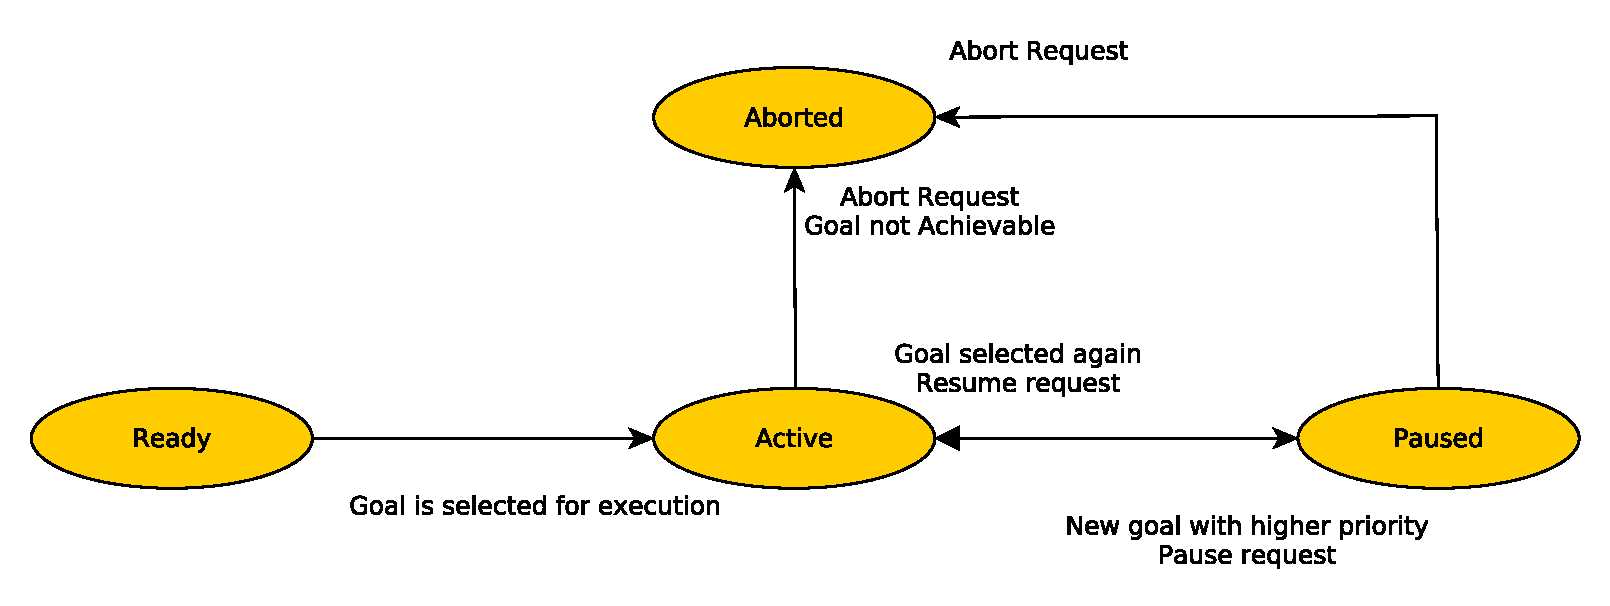
\includegraphics[clip,scale=0.6]{img/goal_management/goal_cycle.pdf}
	\caption{The state machine representing transitions between the statuses of a goal.}
	\label{fig:goal_management-goal_cycle}
\end{figure}



The robot will select a $ready$ goal to become $active$. The $active$ goal is selected by choosing the goal with the highest priority, with random selection used to solve conflicts.

If the robot is executing a plan to achieve a goal, and a new goal with a higher $priority$ becomes $ready$, the current goal becomes $paused$, and the robot considers $active$ the new goal. A goal can also become $aborted$ if it was $active$ and there is no plan to achieve it or if the human requests the robot to abort it. Finally, a goal will transition to the $completed$ state when it has been achieved.

When a goal is selected as active, the robot will contact the Plan Production and Management layer to achieve it, as explained in chapter \ref{chapter:plan_management}.




% Chapter Template

\chapter{Plan Production and Management} % Main chapter title

\label{chapter:plan_management} % Change X to a consecutive number; for referencing this chapter elsewhere, use \ref{ChapterX}

\lhead{Chapter 4. \emph{Plan Production and Management}} % Change X to a consecutive number; this is for the header on each page - perhaps a shortened title

In this chapter, we introduce the Plan Production and Management layer of our system. Section~\ref{sec:plan_management-intro} introduces the subject, with a review on multi-agent planning, explanation, negotiation and plan management. section~\ref{sec:plan_management-overview} shows the main aspects of this component. Our system is able to use different plan management modalities, as explained in ~\ref{sec:plan_management-modalities}. section~\ref{sec:plan_management-human_knowledge} introduce the idea of maintaing the level of knowledge of a user in a task, which will be used both in plan generation and management. section~\ref{sec:plan_management-plan_generation} introduces our task planners, HATP (\ref{subsec:plan_management-hatp}), and HAPP (\ref{subsec:plan_management-happ}), and shows how plans are adapted to the expertise of humans in the  tasks (\ref{subsec:plan_generation-adapting_knowledge}). section~\ref{sec:plan_management-plan_explanation} shows how plans are explained to users, and section ~\ref{sec:plan_management-negotiation} how they are negotiated.  section~\ref{sec:plan_management-plan_manager} introduces the plan management aspects of this layer. We developed different strategies, shown in subsections ~\ref{subsec:plan_management-sequential_plan_management} and ~\ref{subsec:plan_management-adaptive_parallel_plan_manager}. section~\ref{section:plan_management-plan_monitoring} shows how are system is able to monitor human actions and task. Finally section~\ref{sec:plan_management-experiments} details a user study created to evaluate the ability of our system to adapt to users.


\section{Introduction}
\label{sec:plan_management-intro}
\subsection{Cooperation between agents}
Robots can be used to perform a large number of different operations. Some of these will be simple enough that the robot can just achieve its task by performing a prefixed sequence of elementary actions. In other cases, the robot might have to achieve complex goals, which require the ability to create plans and to adapt them to the current state of the world. When cooperating with other agents, the robot has to build a shared plan, which includes the actions that every agent need to perform, in order to coordinate and ensure the corrent achievement of the goal. We can imagine the following process:
\begin{itemize}
	\item The system receives a new goal. This can be directly introduced by a human, or chosen after some kind of reasoning by the robot.
	\item One of the agents (the robot or the humans) proposes a shared plan to achieve the goal, and presents it to the other agents.
	\item The agents negotiate the plan. In some situations, one of the agents might not be able (or might not want) to perform a specific action, or sequence of actions. The agent can refuse the plan, proposing a correction or a completely different plan.
	\item The agents execute the plan. Each agent performs its part of the plan. In addition, agents may check the state of others to monitor the correct execution of their part of the plan or to cordinate with them.
	\item An agent might fail his part of the plan. If this happens the agents need to create a new plan to account for this failure.
 	\item The process continues until the goal is achieved or it becomes unachievable (for example, a needed resource is no longer available).
\end{itemize} 
When humans cooperate this process can be very quick. For simple tasks humans are able to coordinate without explicitly forming a plan, in particular if they are used to cooperating together. Other times, when there are unexpected problems during the execution of a plan, humans are able to quickly readapt their plan, without completely restarting this process. In order to cooperate in a natural way with humans, robots need to reproduce these mechanisms.

\subsection{Multi Agent Planning}
Multi-Agent planning   is an important and studied topic in the AI community \cite{durfee1999survey}. There are several approaches to this problem, using classical or probabilistc planning. There are several issues to consider:
\begin{itemize}
\item Distributed vs Centralized. A multi-agent planner might be distributed, meaning that separate systems plan independently and then communicate to build a shared plan (an idea investigated, for example in \cite{nikolaidis2013cross,guestrin2002distributed} ); or centralized, meaning that a single system plans for all the agents.
\item Coordination. Agents need to coordinate their plans, in particular in the presence of shared resources. Imagine, for example, two agents, Max and Bob, that are using a tool to repair a set of cars. If Max is proceeding faster than Bob and the two do not coordinate, Max might take the tool and leave, starting to repair another car, ignoring the fact that Bob still needs the tool. This example shows that it is important to reason on the duration of actions performed by agents. At the simplest level, agents need to know the advancament of the sub-plan of other agents. More complex reasoning might take into account how long an agent needs to perform a certain sub-task, in order to refine a plan. 
\item Cooperation. Even when performing different sub-tasks of the same plan, agents can help each other, for example by passing items, thus improving the efficiency of the plan. Multi-Agent problems can be loosely or tightly coupled, depending on the quantity of interactions between agents. Some works are not focused specificly on tightly or loosely problems, and try to present a generic approach. \cite{torreno2015approach} proposes a cooperative refinement planning approach, based on the partial-order planning paradigm. In this work each agent refines a centralized plan. Agents are able to exchange information, since the complete world-state might no be observable by all of the agents. Refined plans are then analyzed by each agents, and voted with a democratic leadership approach. Results show that this approach is very efficient at solving loosely coupled problems, but also competent on tightly coupled situations. 

\item Communication and Knowledge. In a multi-agent environment each agent might have an incomplete or incorrent belief on the world, which might lead to wrong or sub-optimal actions. Agents may communicate to progressively build a correct belief model on the state world. 
\end{itemize}

Several approaches has been studied to bring the multi-agent planning problem in a probabilistic framework. \cite{boutilier1999sequential} create a centralized MDP, able to select at each time step actions for every present agent. Dec-POMDP \cite{bernstein2002complexity} and I-POMDP \cite{gmytrasiewicz2005framework} are more complex frameworks, that take into account the belief models of agents. The complexity of these models makes them difficult to use in even moderately difficult scenarios. A solution to this problem is considering simpler problems, where the agents mostly work independently and interact only in limited situations, such as in \cite{melo2013heuristic}.  Since we are more interested in tightly coupled scenarios, where the robot and human interact often, these kind of approaches are not suitable.

\subsection{Plan Explanation and Negotiation}
In order to form  shared plans, agents often communicate, explaining tasks to each other and negotiating to agree on a solution. In \cite{Lallee2013} the authors suggest that joint plans should be fully communicated in order to sustain effective collaboration. 

In a collaborative scenario, all the agents must agree on the shared plan. If there is a disagreement the agents might negotiate to find a nother solution.  This problem has been studied, for example, in \cite{fabregues2014hana}, where the authors present the \HANA system, an architecture that allows agents (robots and humans) to negotiate in competitive and cooperative settings. In HANA agents interact during the whole planning process, proposing solutions while they keep searching for better plans. During this process agents agree on performing specific tasks, which prunes the search space of feasible plan.

\subsection{Plan Management}
Finally, the shared plan needs to be executed. Agents need to perform their part of the plans and to monitor their partners in order to coordinate with them. Two examples of systems able to execute shared plans are  Chaski \cite{shah2011improved} and Pike \cite{levine2014concurrent,karpas2015robust}. 

Chaski is an executive system that enables the robot to anticipate and adapt to other agents actions. Chaski is based on human teamwork strategies, including ideas such least moment commitment, frequent communications on the task status, and considering the consequences of the robot's choices on other agents. Chaski is able to execute plans in two different modalities: Equal Partners and Leader and Assistant. Chaski receives as input a shared plan, including the activities that need to be performed, the capacities of each agents, and the deadlines for these activities. Chaski produced a compact representation of all the possible scheduling of activities, based on this plan, which is used to take decisions on the fly during executing, and to adapt to human choices. Results show that Chaski is able to reduce human's idle time in an equal partners scenario. A possible problem of this approach is that if an agent completely deviates from the chosen plan, the system needs to create a new plan, which needs to be encoded again by the Chaski.

Pike is another executive, able to simultaneously recognize human plans and adapt to them. Pike receives as input a plan, represented as a Temporal Plan Network with Uncertainty (TPNU). Pike represents this plans by considering controllable choices (i.e. actions) for the robot and uncontrollable choices for the human. The idea is considering that these choices are not independent, and in this way the system can infer what actions the human would rationally take to obtain his goal and what actions the robot should take to help him. The system receives a stream of human choices, which allows it to determine the robot's actions. Pike has been tested in simulation and with a real robot with good results, managing, on average, to take decisions with a low latency.

If the human does not follow the TPNU Pike will return a failure. The authors discuss integrating the system with a generative planner in the future to overcome this limitation.

\section{Overview}
\label{sec:plan_management-overview}
Our system presents a planning layer which is able to perform the following tasks:
\begin{itemize}
	\item Interface with external planners in order to create a shared plan. The system has been integrated with a HTN (Hierarchical Task Network) based planner, HATP (Human-Aware Task Planner), and with a multi-agent MDP planner.
	\item Monitor a human plan. Our system is able to monitor other agents' parts of a plan, to cordinate with them and to react when an agent fails an action or his actions diverge from the current plan.
	\item Receive plans from a user. Users can interact with the robot with a tablet application, asking it to execute specific actions or goals.
	\item Executing shared plans in different modalities. The robot can be a leader, assistant, or equal partner of humans during plan management.
\end{itemize}

A number of modules implement this ideas, as shown in figure \ref{fig:plan_management-architecture}:
\begin{itemize}
\item Task Planner. Creates a shared plan for the involved agents.
\item Plan Management. Manages the current plan, interacting with the Execution Management layer to execute the robot's action and with the Situation Assessment layer to monitor human's actions.
\end{itemize}

After receiving a goal from the Goal Management layer, the Plan Management module sends a request to the Task Planner to look for a suitable plan. If there is a plan, depending from the current modality, it will send it to the Plan Management module.. 

\begin{figure}[ht!]
	\centering
	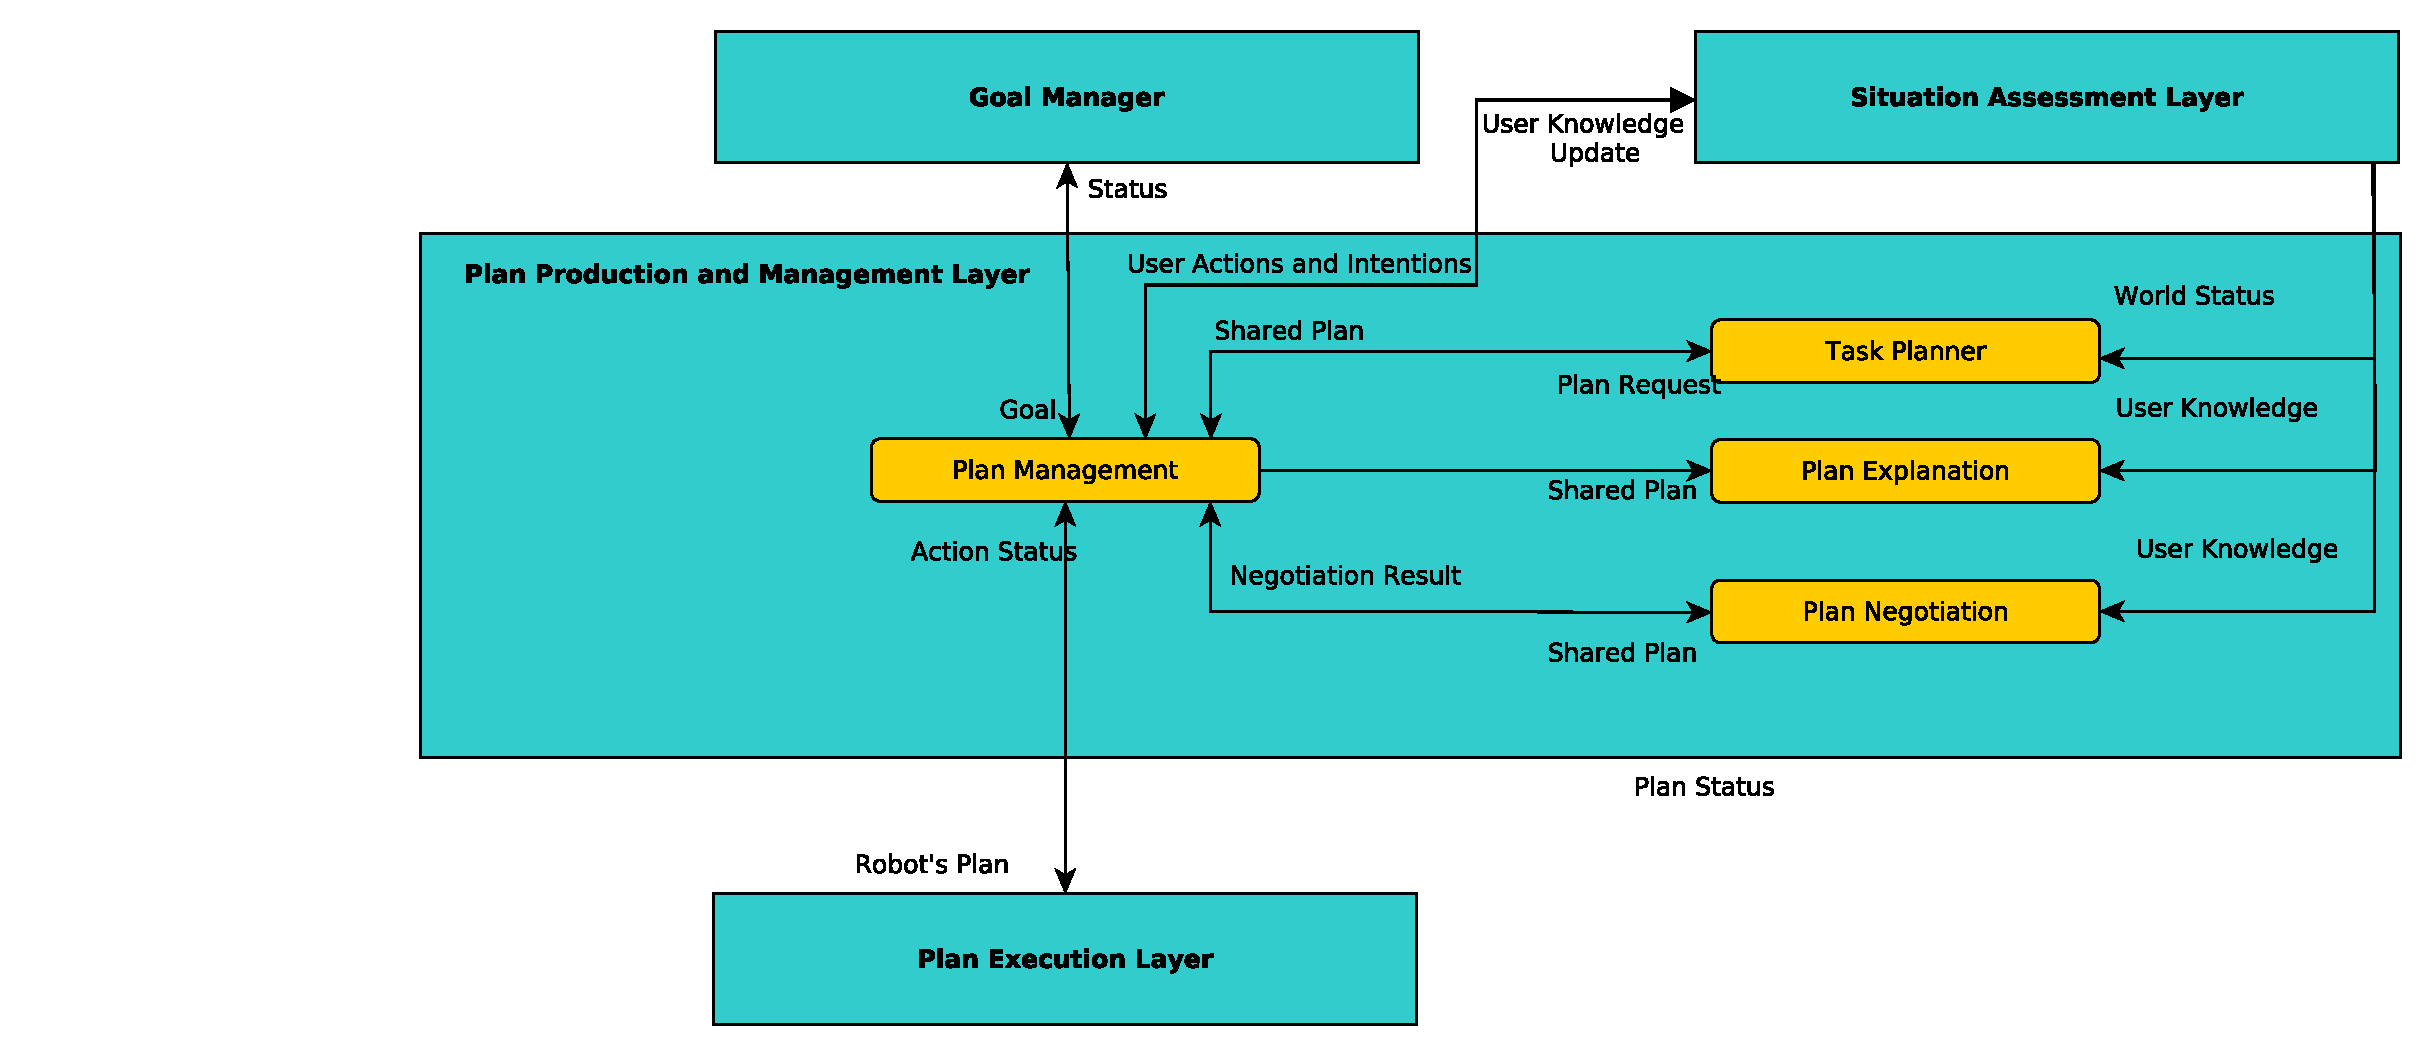
\includegraphics[scale=0.5]{img/plan_management/architecture.pdf}
	\caption[The architecture of the Plan Production and Management layer]{The architecture of the Plan Production and Management layer. Light green rounded rectangles represent modules, while dark green rectangles layers. Arrows represent message exchanged between components, with the label detailing the message.}
	\label{fig:plan_management-architecture}
\end{figure}


Part of this chapter was presented in \cite{Lallement2014,milliez2016using,fioreiser2014}.

\section{Plan Management Modalities}
\label{sec:plan_management-modalities}
When acting together, agents sometimes do not have the same decision power, with one of them assuming the role of a leader. We represent this idea, in our system, by proposing three different modalities: \textit{robot leader}, \textit{human leader}, and \textit{equal qartners}. The robot is able to switch from one modality to another during the execution of a plan. For example, if the current modality is \textit{robot leader} and the Robot receives a command from a user, it will switch to the \textit{human leader} modality, after interrupting its current action.

\subsection{Robot leader}
In this modality the robot, after computing the plan, will explain it, negotiate it and start executing it.
The robot will track the status of humans, informing them of which actions they should execute. This modality can be helpful when interacting with  naive users or in tasks where the robot has a better knowledge of the
domain or of the environment than the other agents.

\subsection{Human Leader}
The human can also create plans, interacting with the robot by using a
tablet application, as explained in section \ref{sec:situation_assessment-communication}. In this modality the robot   
will simply observe the surroundings and wait for user inputs. This modality is always available and has a priority over
the other two modalities. If the robot receives a command from the
application while it is in another modality, it will abandon its current
plan, stopping its actions at a safe point, and then execute the users'
command. We feel that this interaction modality is important for two
different reasons.  First, some users will simply prefer to be in
charge of the execution process, for a matter of personal preference or because they
feel they have a deeper knowledge on how to realize the current task
than the robot. We can picture, for example, industrial or medical
scenarios, where the human is the leader and asks the robot to perform
different tasks to help him, when needed. A second use of this modality is in situations where
the robot does not have  a clear estimation of the users' intentions and
goals. For example, in a domestic environment, a user could decide to
order a robot to bring him a drink, a need that the robot can not always anticipate.

\subsection{Equal Partners}
In the last presented operation modality the robot will try to help
the human to complete a task. At the start of the scenario, the robot
will stand still and observe the environment. After the user takes an
action the robot will calculate a plan and try to help as it can, by
performing actions related to that task and by giving helpful information to
the user, for example to fill gaps in their knowledge. In this modality, 
the robot will not explain or negotiate the current plan and will not warn humans if
their actions differ from the plan computed by the robot.

We feel that, particularly in non-critical tasks, where defining an accurate plan between the partners is not
fundamental, this modality is a very natural way of
interaction between different partners.


\section{Plan Generation}
\label{sec:plan_management-plan_generation}
One of the goals of our system is flexibility; we consider important the possibility to interface with external components. We built an intermediate Plan Generation module that interacts with external planners,  returning  plans represented in a common format that can be handled by the other modules. 

We consider that plans can be decomposed in a set of sub-parts, that we call \textit{tasks}. In general tasks can be decomposed in simpler sub-tasks, until reaching the most basic form of task of a domain, which we call \textit{action}. Both actions and tasks follow the same representations, $(name,preconditions,target,postconditions)$, that we introduced in ~\ref{chap:situation_assessment}. In ~\ref{sec:sec:situation_assessment-intention_recognition} we introduce our intention and action recognition module. In this module, we specified that the system possesses a list of known actions. Every action in a planning domain that can be performed by humans need to be present in the list posseded by the Situation Assessment module. In this way, the system will be able to monitor the execution of actions by humans, with the mechanism of the robot observer.

In some situations, to be more generic, we will use the word \textit{task} to refer to both tasks and actions, since actions are actually tasks that can not be decomposed in the current planning model.

We require that each planner, to interface with our system, provides as input a set of streams, one for each agent. A stream is a sequence of nodes, where each node corresponds to task assigned to be executed by the agent. We introduce causal links between tasks, even of different streams, to ensure synchronization. A causal link $l=(t_1,t_2)$ indicates that  $t_1$ should be execute before action $t_2$. This ensures that all the preconditions to execute $t_2$ are fullfilled. Moreover, if $t_1$ and $t_2$ are executed by different agents, and if there is a shared resource connected to the action, the causal link indicates that the resource will be released by the agent only after $t_1$ is completed. An example of these data structures is shown in figure~\ref{fig:plan_management-plan_structure}.

\begin{figure}[ht!]
 \centering
  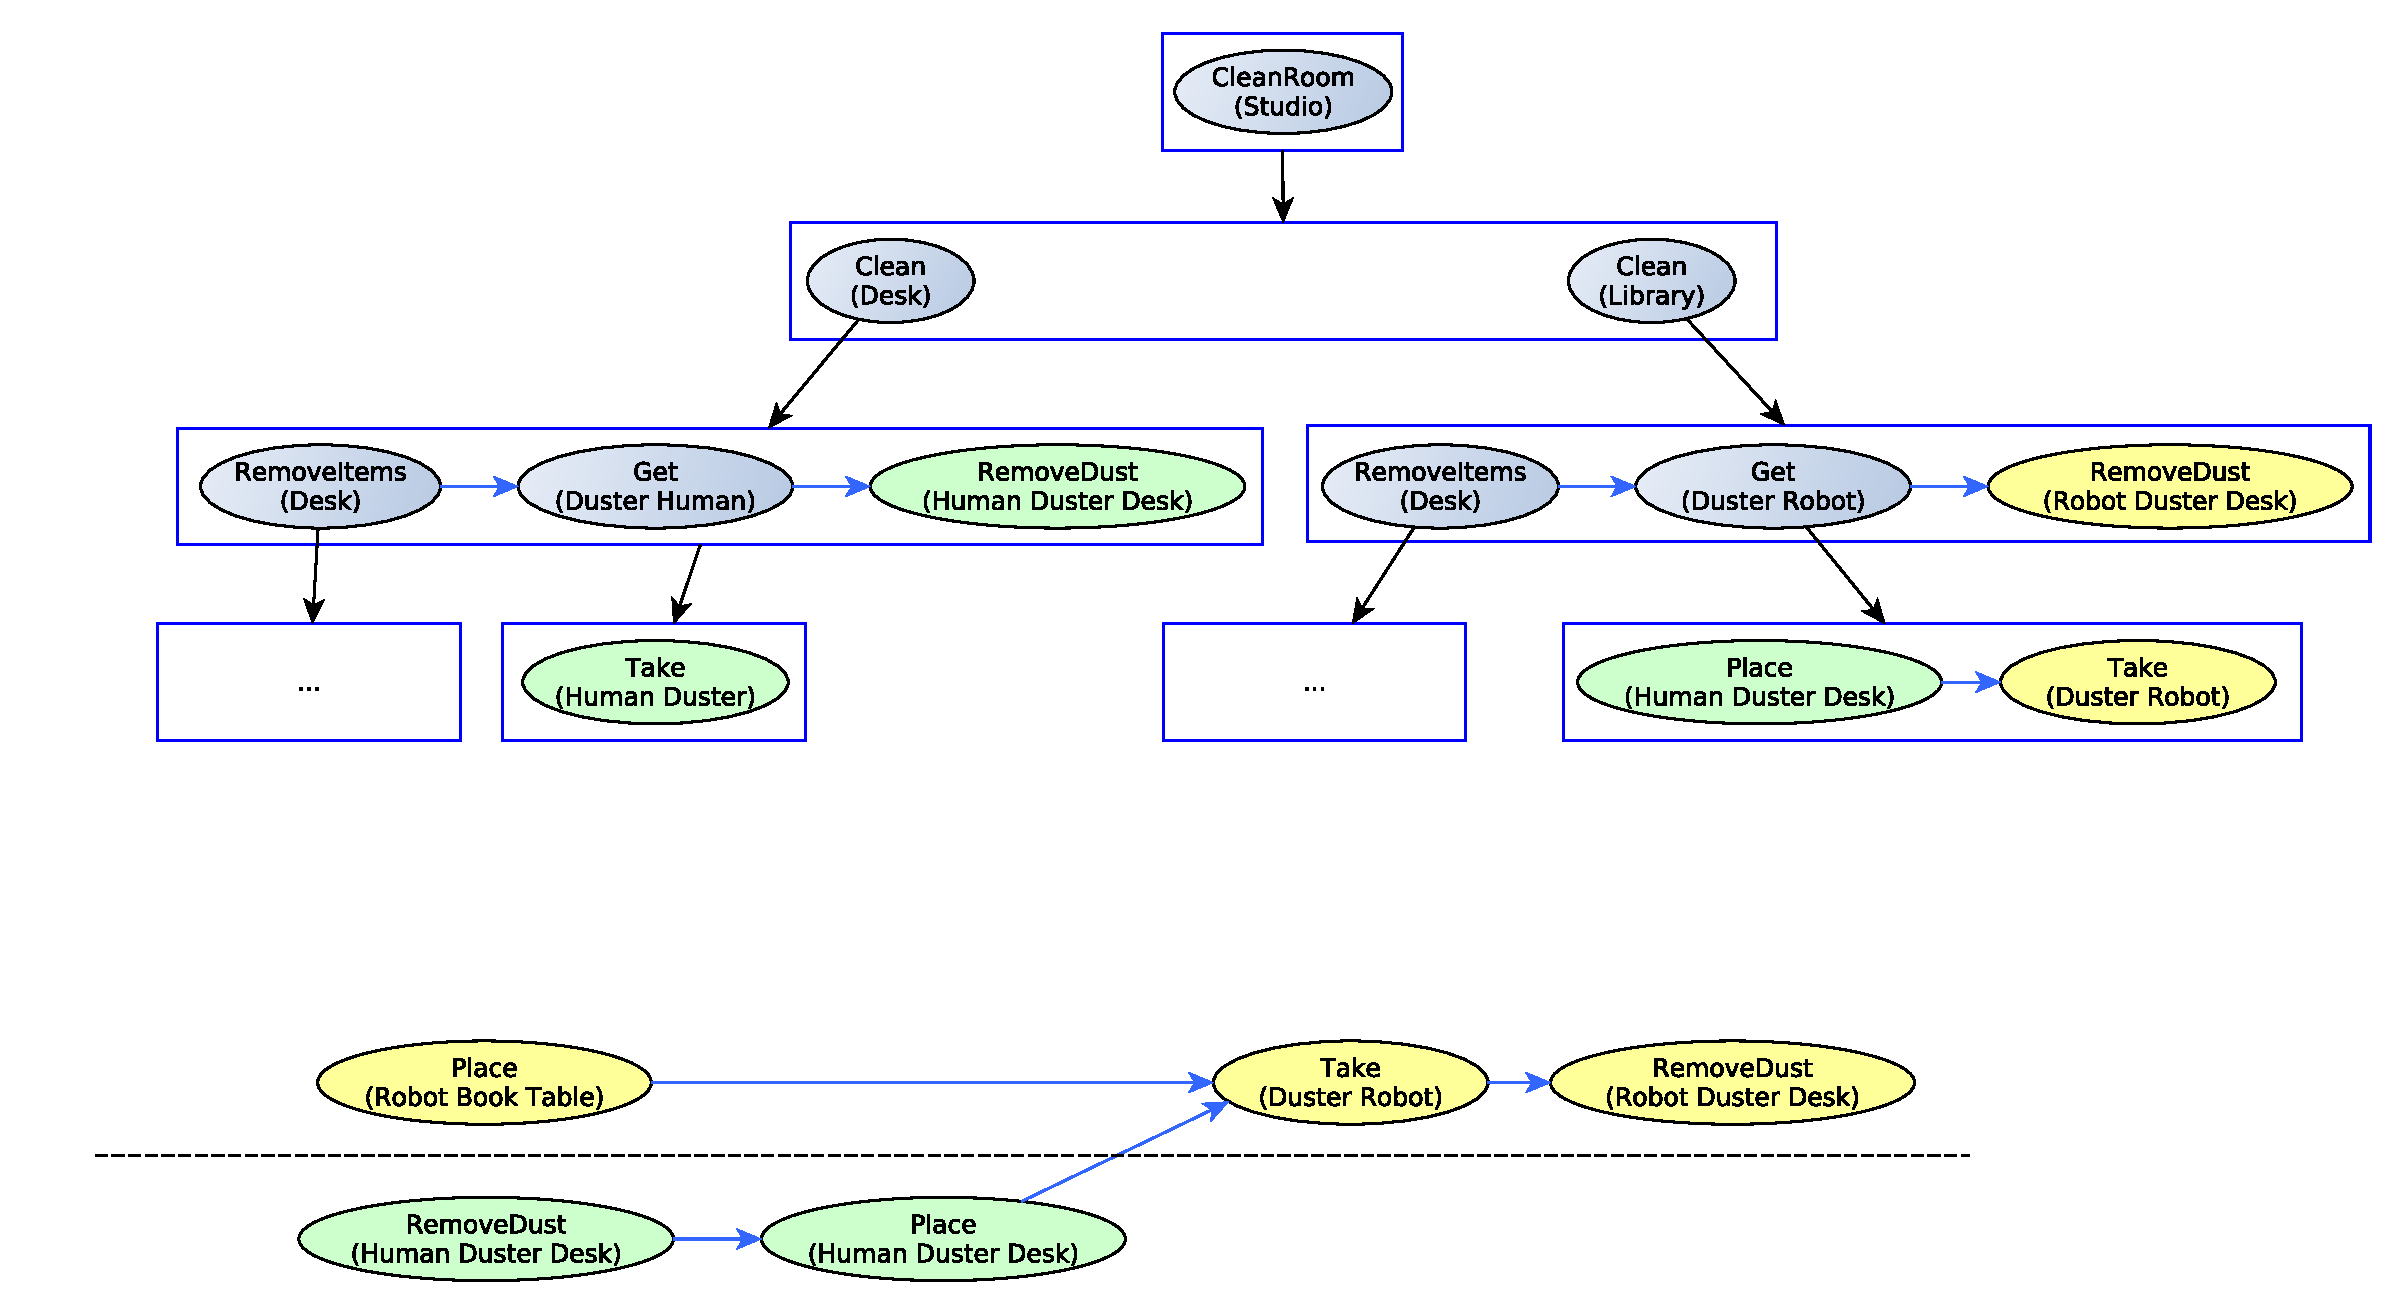
\includegraphics[scale=0.45]{img/plan_management/plan_data_example.pdf}
 \caption[Plan data structures]{a) A HTN plan data structure used in our system, representing a possible way to clean a room
 with two agents, a robot, and a human. Blue ellipses represent tasks, green ellipses represent
 actions assigned to the human, and yellow ellipses actions assigned to the robot. Each decomposition is grouped
 in a blue rectangle. Black arrows link a method to its decomposition, while blue arrows represent causal links. The two squares with a "..." label represent decompositions that are not shown in this picture.
 b) A part of the plan streams associated to the tree data structure. The upper stream represents the robot, and the lower one a human. Notice the causal link between the Place(Human Duster Desk) in the human stream and the Take(Robot Duster) in the robot stream. This link indicates that the robot should wait that the human places the duster before executing the action to take it, ensuring synchronization }
 \label{fig:plan_management-plan_structure}
 \end{figure}


At the moment, we tested two different planners with our system, which will be shown in the next subsections.


\subsection{Human-Aware Task Planner}
\label{subsec:plan_management-hatp}
Computing a plan in complex environments can be very hard and time consuming. A useful approach to reduce the search space in planning is introducing the knowledge of an expert in the system, in order to guide the planner toward desirable states. An implementation of this idea is HTN, where the domain expert specifies a hierarchical library of operations, called methods, when the operation is a node in the hierarchy, and actions, when the operation is a leaf. HATP \cite{Lallement2014} is a planning framework that extends HTN for human-robot interaction problems. Among the capacities of HATP we can find:
\begin{itemize}
\item Multi-Agent. HATP is able to include different agents in its domain, specifying which actions each one can execute. HATP is able to plan for different agents at the same time, humans and robots. The planner can also compute ``joint actions", that involves more agents at the same time.
\item Social Rules. The domain expert can introduce a set of rules, which represent desirable behaviors, for example to distribute in different ways operations between agents, or to avoid specific sequences of actions. Social rules help producing human-aware plans, that avoid behaviors that can be considered rude as humans. Using social rules, HATP can also balance in different ways the amount of effort of each agent in the plan. For example, we might choose that the human should have a minimum effort in the plan, or that the effort should be balanced between the human and the robot.
\item Cost Driven. The domain expert can specify a cost for actions. Plan pruning allows to explore more efficiently the search space, discarding paths that are not promising.
\end{itemize} 

Plans are represented as an HTN tree decomposition and as a set of streams, one per agent, which shows which actions each agent needs to perform. Casual links are introduced between streams to ensure synchronization.

\section{Plan Management}
\label{sec:plan_management-plan_manager}

The Plan Management algorithm will be divided in different threads of execution, one for each agent. We will now explain this algorithm, which is shown in figure \ref{fig:plan_management-manage_plan_not_leader}.
\begin{itemize}
  \item Each thread executes the part of the plan of an agent, composed by $n$ different actions.
  \item For each action, for every causal link $(a_i,a_n$), where $a_n$ is the current action, and $a_i$ is another action, the plan manager waits until $a_i$ is completed, or there is an error. This is handled in the \textit{waitCasualLinks} procedure.
  \item When all the causal links have been satisfied, the execute\textbackslash monitor procedure is called, depending if the thread is managing the robot or another agent. The \textit{executeAction} operation interacts with the Execution Management layer to complete the action, while the MonitorAction operation with the Situation Assessment layer.
  \item If these procedures succed, the plan manager switches to the next action, otherwise it returns a failure.
  \item The process is continued until there is a failure or the plan for the current agent is completed.
\end{itemize} 

\begin{figure}[ht!]
 \centering
 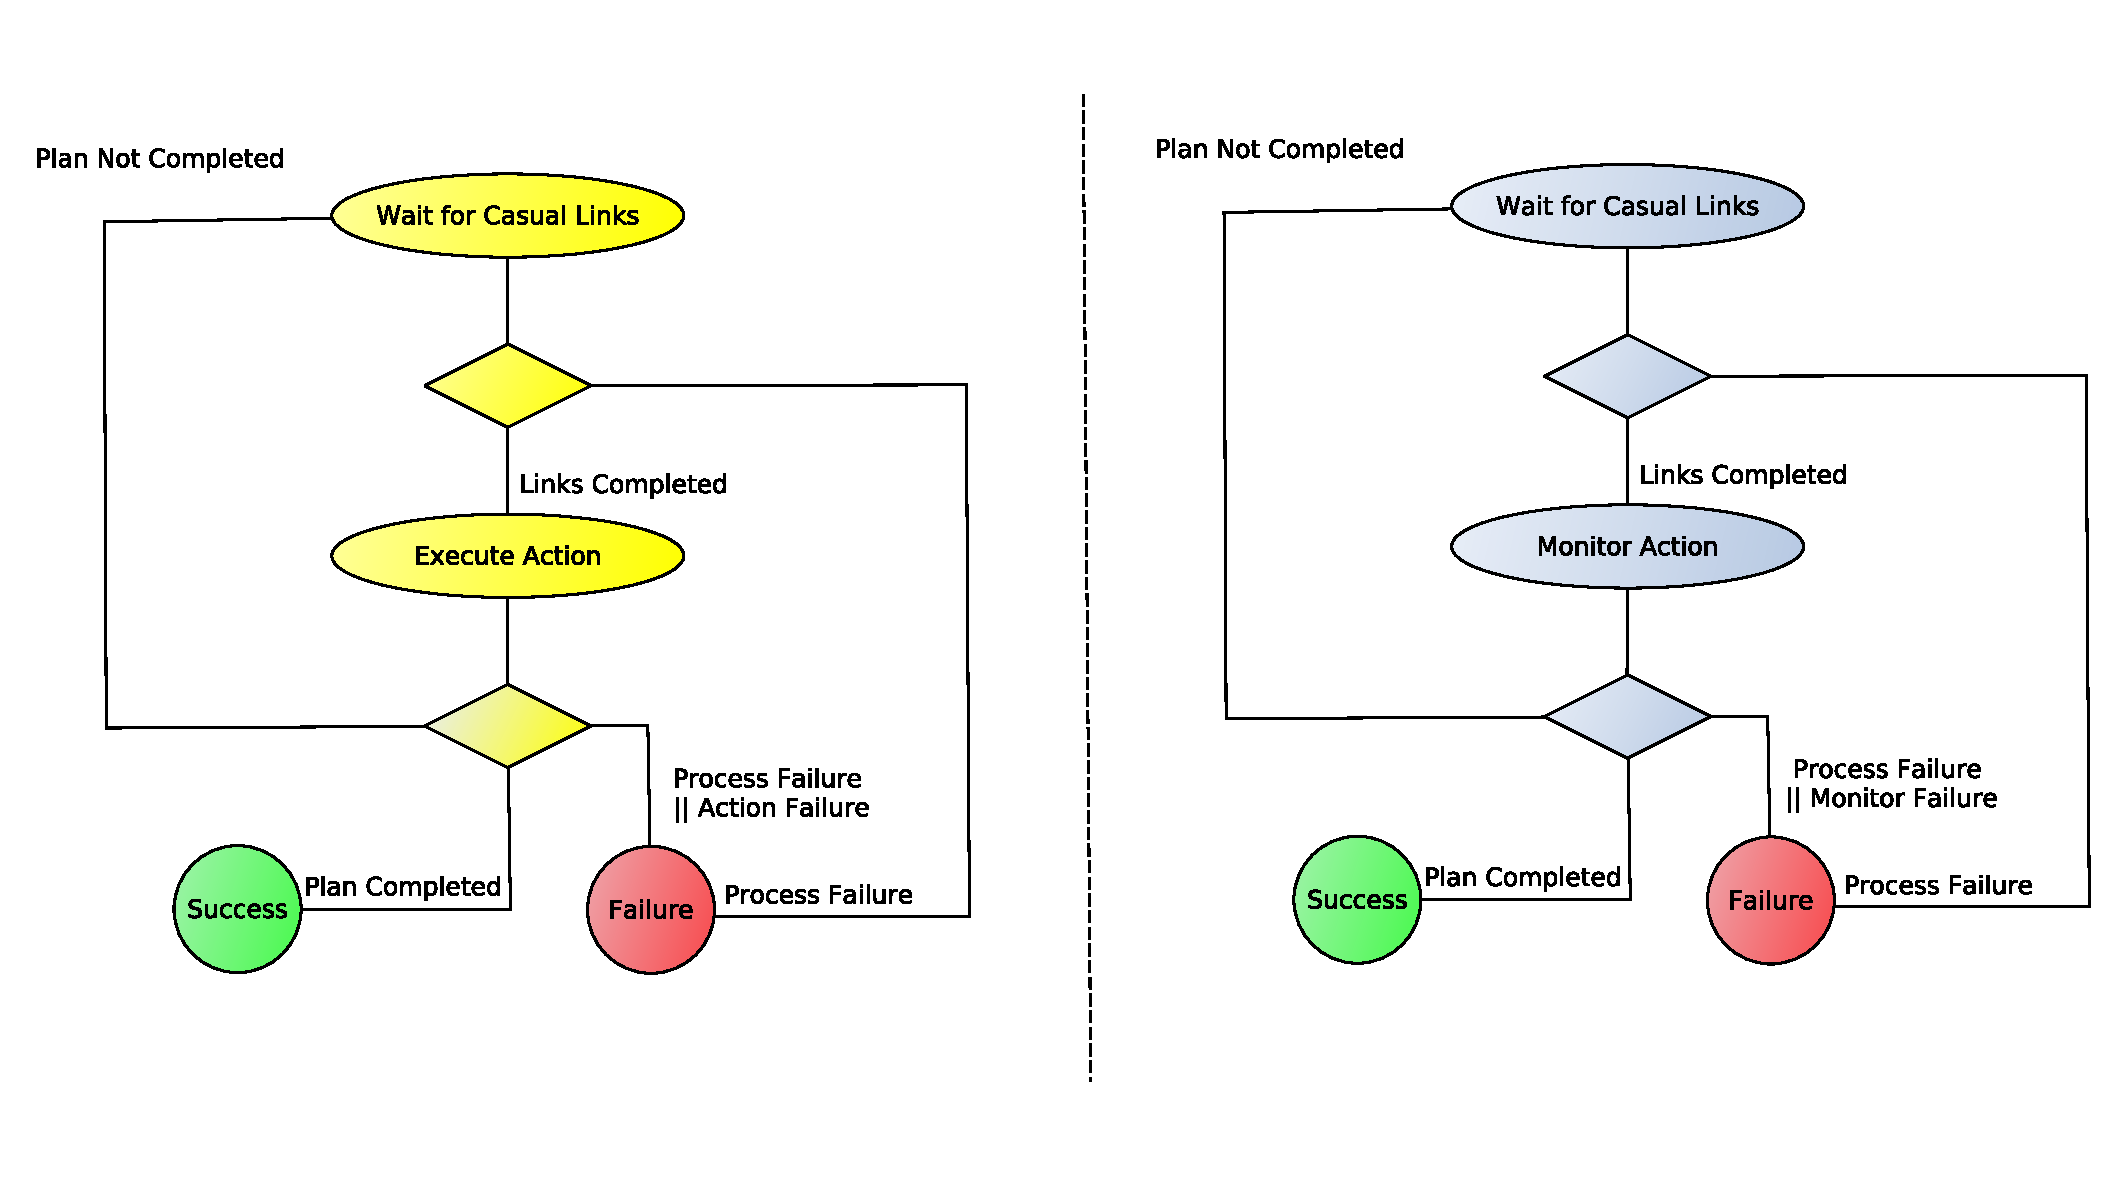
\includegraphics[scale=0.6]{img/plan_management/manage_plan_not_leader.pdf}
 \caption[Plan Management when the robot is not leader]{The plan management algorithm used when the current modality is not \textit{robot leader}. The algorithm is composed by different threads, one for each agent. In this instance, the upper lane represents the robot's management thread, while the bottom a human's management thread. Elliptic nodes represent operations. Diamond nodes, representing divergences in the algorithm, where adding only when they could simplify the understanding of the algorithm. Arrows imply a transition between nodes, with the label of the arrow representing the condition of the transition, when present. The absence of a label implies that a transition is always applied. The blue circle node, called ``start", represents the start of the algorithm. The green and red circle node, instead, represent the success or failure of the algorithm.}
 \label{fig:plan_management-manage_plan_not_leader}
 \end{figure}

Failures in the algorithm lead to a replan request. If a new plan is found, the algorithm starts again, otherwhise the goal is considered failed.

In this modality, the robot will expect users to execute a specific set of tasks, warning them if they do not respect this allocation. Sometimes, the robot will choose the decomposition of the tasks that should be executed by a user, but, when the partner is competent enough in a high-level task,  we may want to allow him the flexibility to execute it as he sees fit. 

\section{Task Monitoring}
\label{section:plan_management-plan_monitoring}

\subsection{Introduction}
During the execution of a plan, the robot will monitor other human partners. In general, having a shared plan, the robot knows what is the human's next expected action, and can monitor if it is accomplished. Plan monitoring poses a number of different issues:
\begin{itemize}
\item Understanding when the next expected action has been performed. In some situations the robot will monitor the execution of a specific action. In this event, it needs to understand when the action has been completed.
\item Understanding when the next expected task has been performed. In some situations, the robot wants to give a human cooperator the freedom to perform a subtask has he sees fit. This is a more complex problem than monitoring a specific action, since the robot needs to reason on the results of sequences of actions.
\item Evaluating the human engagement in the current task. The robot needs to understand if the human is trying to accomplish its current task, if he momentarily interrupted it, or if he abandoned it.
\end{itemize}

At the moment, we have implemented and integrated in our system only monitoring of actions. We will show how we include this idea, and then illustrate in the next chapter how we could extend our system to monitor tasks and evaluate the human engagement in the current task.

\subsection{Monitoring Actions}
At all time, as previously explained in ~\ref{chapter:situation_assessment}, the system constantly observes the environment, monitoring which actions are executed. As previously said, each action that can be executed by a human needs to have the same representation in the Situation Assessment and Plan Management layers. When the plan manager needs to monitor an action $a$ of a human stream, its $preconditions$ will be satisfied (since, if we are monitoring $a$, all of its causal links have been already satisfied). This means that $a$ will be in the IG for the human, which will be monitoring its execution.

The Plan Manager will wait for Situation Assessement to infer that an action has been performed. If the action is different from $a$, it will return an error, prompting a replan. Otherwise, the plan management will continue with the next action in the stream, if any.

For example, let us imagine a scenario where Greg is near a table, with a \textit{bottle} and a \textit{book} on top. Let us say that, at the moment, Greg can execute three actions: \textit{take book}, \textit{take bottle}, and \textit{move kitchen}. The current IG for Greg will include these actions, as well as observations to infer their execution. In this example, Greg is following the stream shown in figure. %bla.
Greg has just completed the action \textit{move to table}, and should now execute the action \textit{take bottle}, if he follows this plan. If the system infers that Greg executes \textit{take book} or \textit{move kitchen}, the plan manager will replan, since Greg executed a different action that the one that was expected. If Greg executes \textit{take book}, the stream will move to the next action, which is \textit{move kitchen}.

%ADD EXPLANATION TO SITUATION ASSESSMENT ON WHY WE USE PROBABILITIES IN ACTION RECOGNITION, and how we would use them

\subsection{Monitoring and Unseen Actions}
Often, in cooperative tasks, agents will operate in different locations, and so they can not observe each other actions all the time. Perhaps one of the agents is cooking in the kitchen,  while the robot is preparing the table for dinner. While we do not deal, in this work, with these issues, there are several studies on plan recognition in partially observable environments, like \cite{geib2005partial}.

% Chapter Template

\chapter{Task Execution} % Main chapter title

\label{chapter:plan_execution} % Change X to a consecutive number; for referencing this chapter elsewhere, use \ref{ChapterX}

\lhead{Chapter 5. \emph{Task Execution}} % Change X to a consecutive number; this is for the header on each page - perhaps a shortened title

This chapter shows the Task Execution layer of our system. Section \ref{sec:plan_execution-intro} introduces the subject. Section \ref{sec:plan_execution-overview} shows an overview of this layer, with its characteristics and components. Section \ref{sec:plan_execution-action_executor} shows the main aspects of the Action Execution module, while \ref{sec:plan_execution-collaborative_planners} shows the framework we use to execute human-robot joint actions.


\section{Introduction}
\label{sec:plan_execution-intro}
Acting in a human-crowded environment is a difficult problem. Even when acting independently, the robot needs to ensure human safety, by taking others into account when planning and stopping if its actions could bring harm; to perform legible movements, so that its actions can be understood by humans (studied, for example, in \cite{dragan2013legibility}); and to be robust, trying to complete its task even in front of unexpected conditions. 

These issues show us that humans should not be treated as simple obstacles by the robot, but need specialized reasoning and execution algorithms.

When performing a cooperative action with the human the robot needs to continuously monitor its partner, checking if he is involved in the task, stopping to wait for him, adapting its movements, and eventually abandoning the task. For example, if the robot is giving an object to a human, it will have to choose a position for its arm where the human can easily reach the object, change this position if the human is moving, and abandon the task if the human leaves the area.

\cite{bussy2012proactive} studied how to execute a transportation scenario jointly with a human partner, but the work is based more on haptic and control issues than actual reasoning, an area of the problem not deeply investigated.

\section{Overview}
\label{sec:plan_execution-overview}

We built an execution layer with different characteristics:
\begin{itemize}
\item Flexibility. The system is built in order to be easily expandable, adding new actions, without having an impact on the rest of the architecture.
\item Human-Awareness. The system is able to take humans into account during planning, considering aspects such as the visibility of the robot, the legibility of its motions, and the confort of the human. Human-Awareness is maintained during the execution of motions, stopping the robot if its movements could endanger a human.
\item Support for joint actions . The system supports joint actions, by specifically representing them in a special framework. 
%rewrite what is a joint action for us
\end{itemize}

These ideas are represented in the following modules, as shown in figure~\ref{fig:plan_execution:architecture}.
\begin{itemize}
	\item Action Executor. This module executes the robot's actions in a robust, human-aware, and flexible way.
	\item Collaborative Planners. This set of planners are used to execute human-robot joint actions, allowing the robot to adapt its actions to the collaborators.
	\item Motion Planners and Executors. These planners are in charge of choosing trajectories for the robot, taking into account the environment and the present agents. We will not discuss this component, as it is outside the boundaries of this work. More details can be found in \cite{Sisbot2008,Mainprice2011,Pandey2010}.
\end{itemize}


\begin{figure}[h!]
	\centering
	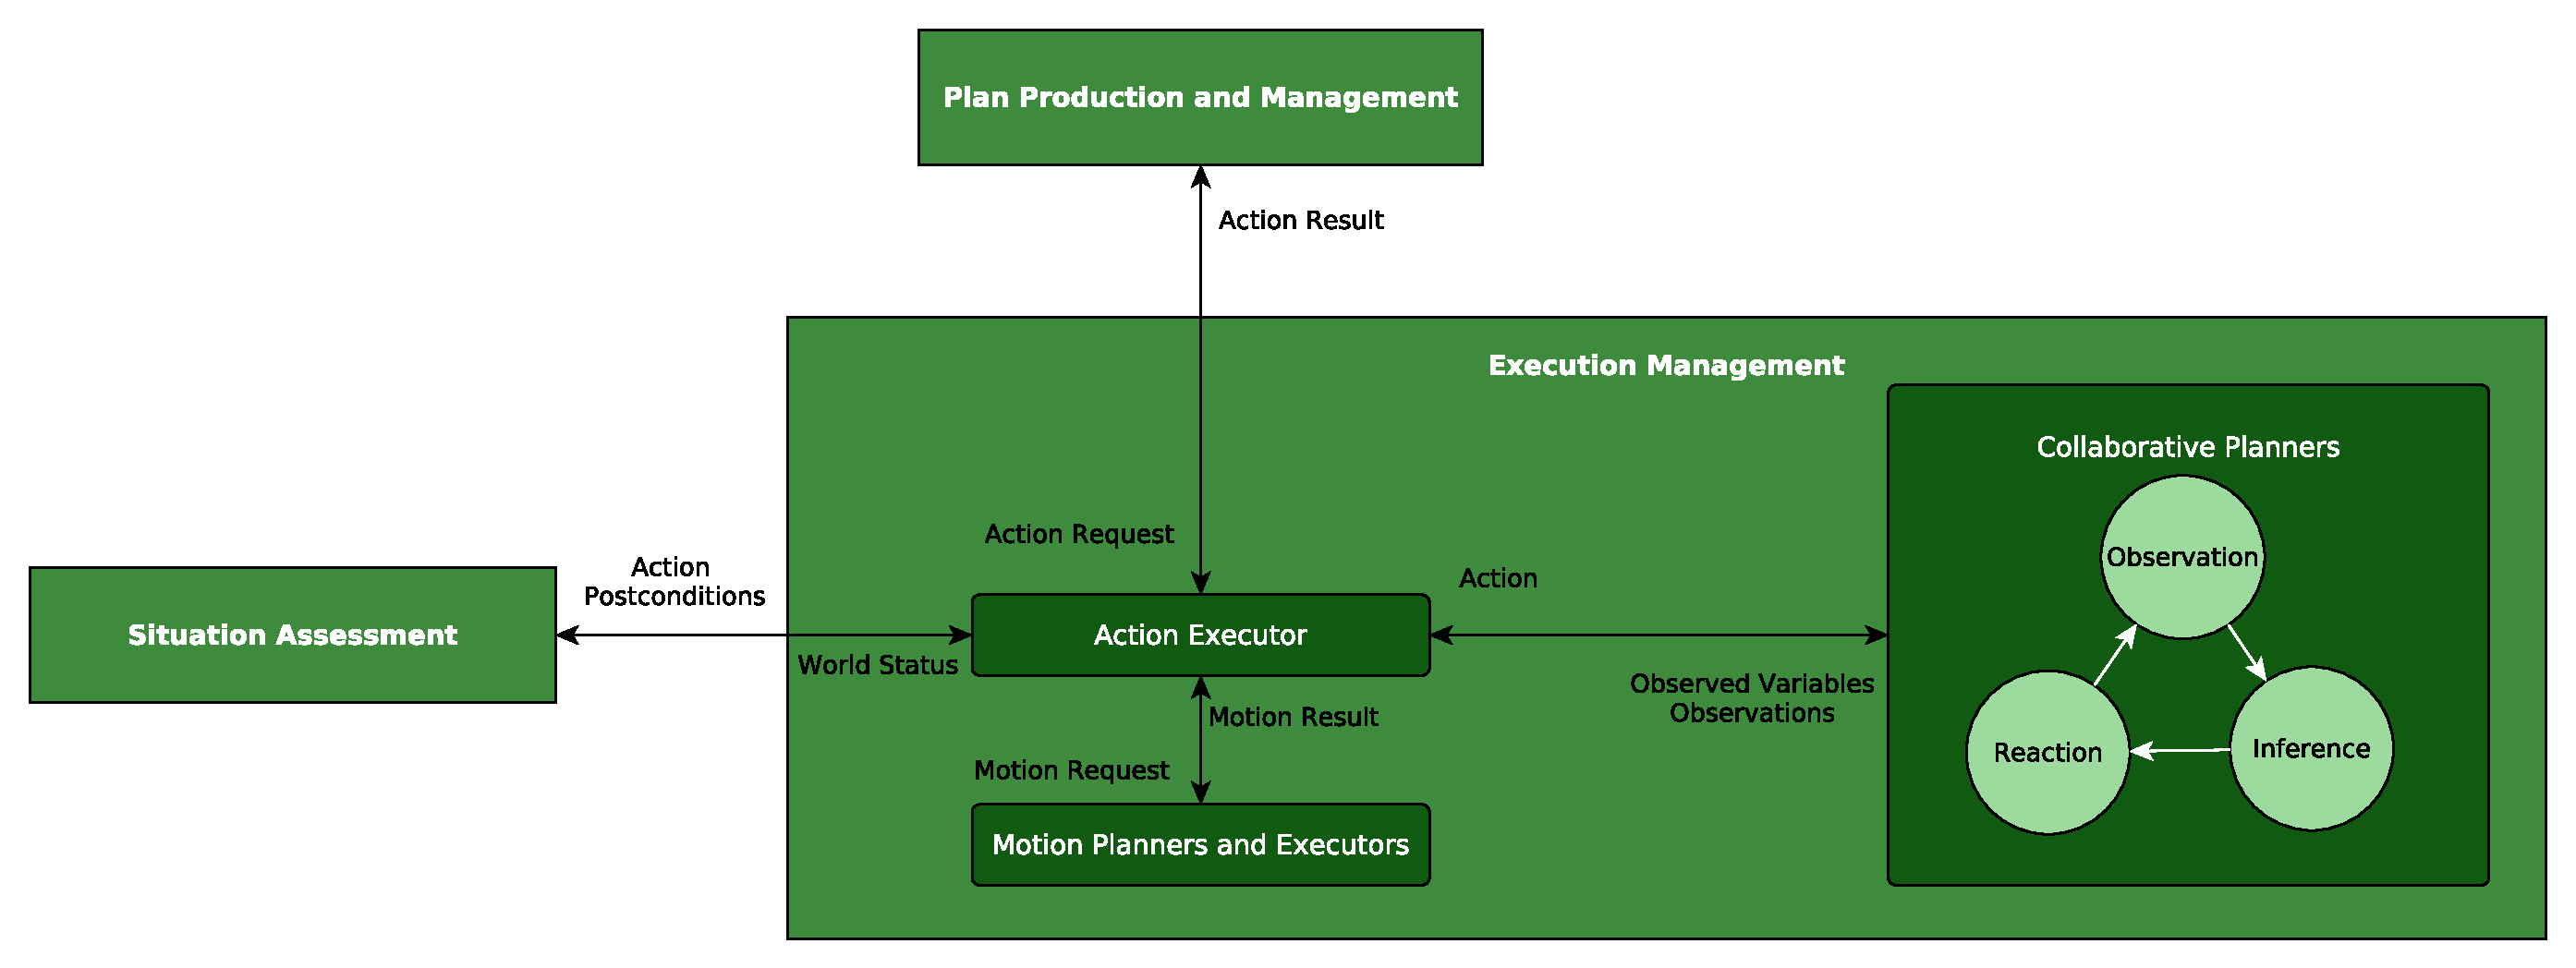
\includegraphics[clip,scale=0.38]{img/plan_execution/architecture.pdf}
	\caption[The architecture of the Execution Management layer]{The architecture of the Execution Management layer. Dark green rectangles represent modules, while light green rectangles layers. Arrows represent message exchanged between components, with the label detailing the message. The white ellipses represens, and their arrows, represent the process of the Collaborative Planners, explained in Section \ref{sec:plan_execution-collaborative_planners} }
	\label{fig:plan_execution:architecture}
\end{figure}

%fix figure


Parts of this chapter where presented in~\cite{fioreiser2014}.

\section{Action Executor}
\label{sec:plan_execution-action_executor}
The action executor handles action requests from the Plan Production and Management layer. Each action, as explained in subsection~\ref{sec:situation_assessment-belief_management}, is a tuple $(name, preconditions, target, postconditions)$. The execution of an action is handled in several steps:
\begin{itemize}
\item Check Preconditions. The system can check if the preconditions of the actions are valid by sending a query to the Situation Assessment layer. If the preconditions are not valid, the module returns an error.
\item Execute Action. The action is executed, by communicating with the Motion Planners and Executors and, if the current action is a joint action, with the Collaborative Planners.
\item Set Postconditions. After the action is completed, its $postconditions$ are set in the Database of the Situation Assessment Layer.
\end{itemize}

The execution of an action can fail, and in that case the world status is updated consequently. For example, if the robot was trying to pick an object, and the action fails because the robot can not find a motion to grab it, the object will be considered as \textit{not reachable} by the robot in the current world status. When the Plan Management and Production replans, the system could look for a plan where the robot changes position and tries again the pick, or even asks another agent to give him the object.

Actions can be paused and resumed, for example because a human steps in the trajectory planned by the robot. The robot is also able to show some social clues during an action, for example by moving its head toward the action's $target$. 

\section{Collaborative Planners} 
\label{sec:plan_execution-collaborative_planners}
When executing joint actions with humans, the robot needs to continuously observe its partner and react appropriately. The robot's action should be based on different aspects. First of all, the robot should act differently depending on the current status and level of advancement of the task. Second, the robot should consider the status of the world, in order to take appropriate actions. Then, as we said, the robot should observe its partner's behavior, which can give different information. Of course, the robot should coordinate with the human's movements. For example, if the two agents are performing an handover, and the human extends his hand, the robot should extend its arm to bring the object in a reachable position.

Observing the human's action can give us more subtle information, that represent how much he is engaged in the task. For example, in the case of the handover, if the human is oriented toward the robot and extending his hand, we can assume that the human is currently engaged and cooperating. If, instead, the human is looking in another direction, or moving away, we can infer that he is currently doing something else, and perhaps has even abandoned the task.

To reason on all these variables and produce an appropriate reaction, we introduced a special framework to manage cooperative actions, called the Collaborative Planners, based on hierarchical Mixed Observability Markov Decision Processes (MOMDP). Using an MOMDP we can model both observed variables, like the task and world status, and hidden variables, like the engagement level of the human, which we can measure from observations. Using a hierarchy of models, as explained in \cite{pineau2001hierarchical}, we can represent complex scenarios and tasks with smaller, simpler models, that can be solved more easily, and expand them by adding more actions and complex behaviors as we see fit.

When the system is executing a joint action between the robot and a human, the Action Executor will contact the related Collaborative Planner.  The Action Executor will send requests containing the observations and observed variables, used to update the MMODPs, and the planner will return a sub-action to execute. To maintain this model generic the Collaborative Planners will output high-level actions, which the Action Executor will adapt to the current situation. This process will continue until the planner reaches a goal states, chooses to abandon the task, or there is a failure.

For example, if the robot is giving a bottle to a human, the related Collaborative Planner will receive information such as the human's distance, orientation, and the pose of his arm, in order to compute if he is involved in the action. Depending on these information, the planner could choose high-level actions like \textit{continue}, which would prompt the robot to extend its arm or release the bottle, 

\subsection{Handover Collaboration Planner}
\label{subsec:case_study-helper-handover}
We implemented a MOMDP model to handle handovers between humans and robots. This model will output high-level actions, adapted by the Action Executor, depending on the current situation. Decisions will be made based on the following variables:

\begin{itemize}
\item The status of advancement of the task. This variables, whose values are \textit{\{not\_completed, touching, completed\}}, is set by the Action Executor module, in the Execution Management layer, depending on the current advancement of the task. The variable will be set as $completed$ when the handover has been performed, $touching$ when the robot detects pressure on the gripper used for the handover, and $not\_completed$ otherwise. 
\item The quality of commitment of the user. This variable has the same meaning as in the collaborative planner for guiding presented in \ref{subsec:case_study-spencer-collaborative_guide_planner} and can assume the same values, but is estimated from different variables. We will still consider the distance and orientation of the human toward the robot, but also the pose of its arm, particularly if its extended toward the robot. 
\item A timer. The variable is used in the same way as in the collaborative planner for guiding, presented in subsection~\ref{subsec:case_study-spencer-collaborative_guide_planner}.
\end{itemize}

The possible actions of this model are the following:
\begin{itemize}
\item Continue. The Action Executor will continue with the handover, which, depending on the situation, will prompt the system to extend the arm or activate the gripper.
\item Wait. The system will wait for the user if he is not engaged in the task.
\item Abandon. The system will abandon the task when the user is no longer interested in performing it. 
\end{itemize} 


% Chapter Template

\chapter{Case Study} % Main chapter title

\label{chapter:case_study} % Change X to a consecutive number; for referencing this chapter elsewhere, use \ref{ChapterX}

\lhead{Chapter . \emph{Case Study}} % Change X to a consecutive number; this is for the header on each page - perhaps a shortened title


\section{Human-Aware Robot Guide}
\subsection{Introduction}
\subsubsection{Overview on the topic}
One interesting problem in human-robot interaction is developing robots able to guide humans, by offering a tour of attractions in an area or simply by helping humans to reach a destination.
A generic mobile robot platform should possess a vast set of skills, which includes advanced perception, motion planning, and task planning. These skills are not enough for a robot guide, which is deployed in highly dynamic human environments, and need to be complemented with human-aware behaviors.

%Examples
Different robot guides have been studied and developed, starting with pioneers like Rhino and Minerva \cite{thrun2000probabilistic}.  Few systems have actually been deployed for long period of time in human environments. Rackhman \cite{clodic2006rackham}, a museum guide with human-aware behaviors, is an example of such system, and has been deployed in a science museum for several months. Another example of robot guide was developed in \cite{bueno2011autonomous}, where the robot is integrated  in a smart museum environment, using virtual avatars with human-aware interfaces, associated to exhibitions, in order to convey information to the users. After these first experiments, several researchers have tried to focus on the social aspects of the problem, which are especially important if the robot needs to offer information. Studies like \cite{yousuf2012development,evers2014development} focus on how the robot should address humans, concentrating on spatial relationships and on how the robot can convey information.

Building and using mental models of users is particularly important in these scenarios, particularly if we are developing a proactive robot, which need to be able to approach people in order to offer its services, and to monitor their level of interest in the interaction. \cite{Jensen2005} presents an assessment of human-robot interaction during an exhibition, where perceptual and task related data are used to compute an internal state according to the scenario. With these information, the robot can compute a new emotional state and interact accordingly with users.
In \cite{rashed2015toward}, a robot guide is able to infer people intention by studying their trajectories. The authors conducted experiments in a museum, managing to classify user trajectories in three classes and developing a method to identify participants that may need guidance. 

Recently there has been emphasis on robot navigation algorithms that explicitly reason about human beings in the environment differently from other static or dynamic obstacles. Starting from \textit{Proxemics}, researchers have investigated explicit social signals based on human-posture and affordance of the environment to improve legibility of robot motion. For detailed discussion on human-aware navigation algorithms we refer the readers to \cite{kruse2013human,rios-ijsr-2014}. Human-aware navigation in a museum situation was studied in \cite{samejima2015building}, where the authors build environmental maps, which include information learnt from human trajectories and postures, in order to plan safe paths that do not disturb humans present in the area. 

The robot guide scenario can become more complex if we consider not only single humans, but groups. Humans, in fact, tend to naturally form groups, which can be classified in different types, based on their size, on their level of cohesion, on their duration, and other factors \cite{forsyth2009group}.  Studying group formations is a complex problem, since the robot must be able to detect humans, which can be occluded in populated environments, and to model their social interactions, which can be ambiguous. One of the most powerful and expressive social cues is distance, used in different works to track social relationship, like \cite{luber2013multi}. 

\subsubsection{Motivations}
We believe that most robot guide systems are focusing on the social aspects of the problem, and on human-aware navigation, without fully considering the fundamental aspects of joint actions. Guiding is a collaborative task, where the robot does not need only to reach a destination, but also to ensure that its followers reach it, while providing a socially acceptable experience to them. In order to achieve this goal, the robot needs to constantly monitor its users, to adapt to their behaviors and to be ready to proactively help them.

The european project SPENCER \footnote{http://www.spencer.eu/} was born with the idea to study social awareness issues in human-robot interaction, and particularly in the application of a robot guide. This project aimed at joining complex robotic algorithms  with social signal processing, by modeling people not at object, but as entities with relationship, social rules, and culturally diverse background. The final goal of the project was deploying a robot guide, in collaboration with the KLM airline, in the Schiphol airport of Amsterdam, performing user studies on real passengers to evaluate the validity of the system.

We applied our system to this framework, creating a human-aware robot guide which is able to lead a group of people to a destination. More particularly, the originality of our approach is that the robot is able to show both adaptive and a proactive behaviors. The robot will try, while guiding, to select a speed that pleases its users, when adapting, or to propose a new speed, using environmental and task related stimulus. Finally, our system will proactively try to engage members of the group if it detects they need assistance. 

\subsection{Building a Robot Guide}
In order to adapt our system to the robot guide scenario we had to enhance several modules, as shown in Figure \ref{fig:case_study-spencer-architecture}: 
\begin{itemize}
\item The user is able to interact with the robot by using a tactile interface on its front. We updated our human interface to reflect the commands that the user is able to use.
\item in this scenario we are not really interested in the intention recognition skills that we developed in Chapter \ref{chapter:situation_assessment}. In an airport there are no complex sequence of actions that humans need to perform and we will evaluate users' intentions by their trajectories and the surrounding environment. We develope an Environment-Based Intention Situation Assessment module to enhance our Situation Assessment Layer, presented in Subsection \ref{subsec:case_study-spencer-intention}. This module is able to 
\item Similarly, task planning and plan management is quite simple in this scenario. The robot will mostly vary its paths in the environment, using similar plans. We developed an A*-based task planner, which is able to find a path in a semantic map, to guide users to their destination, presented in Subsection \ref{subsec:case_study-spencer-planner}.
\item The main work, in this application, has been creating a Collaborative Planner to guide users in a human-aware way. Using this planner, our robot is able to adapt itself to users actions, or to proactively propose new behaviors. This planner is presented in Subsection \ref{subsec:case_study-spencer-guiding_users}.
\end{itemize} 

\begin{figure}[ht!]
	\centering
	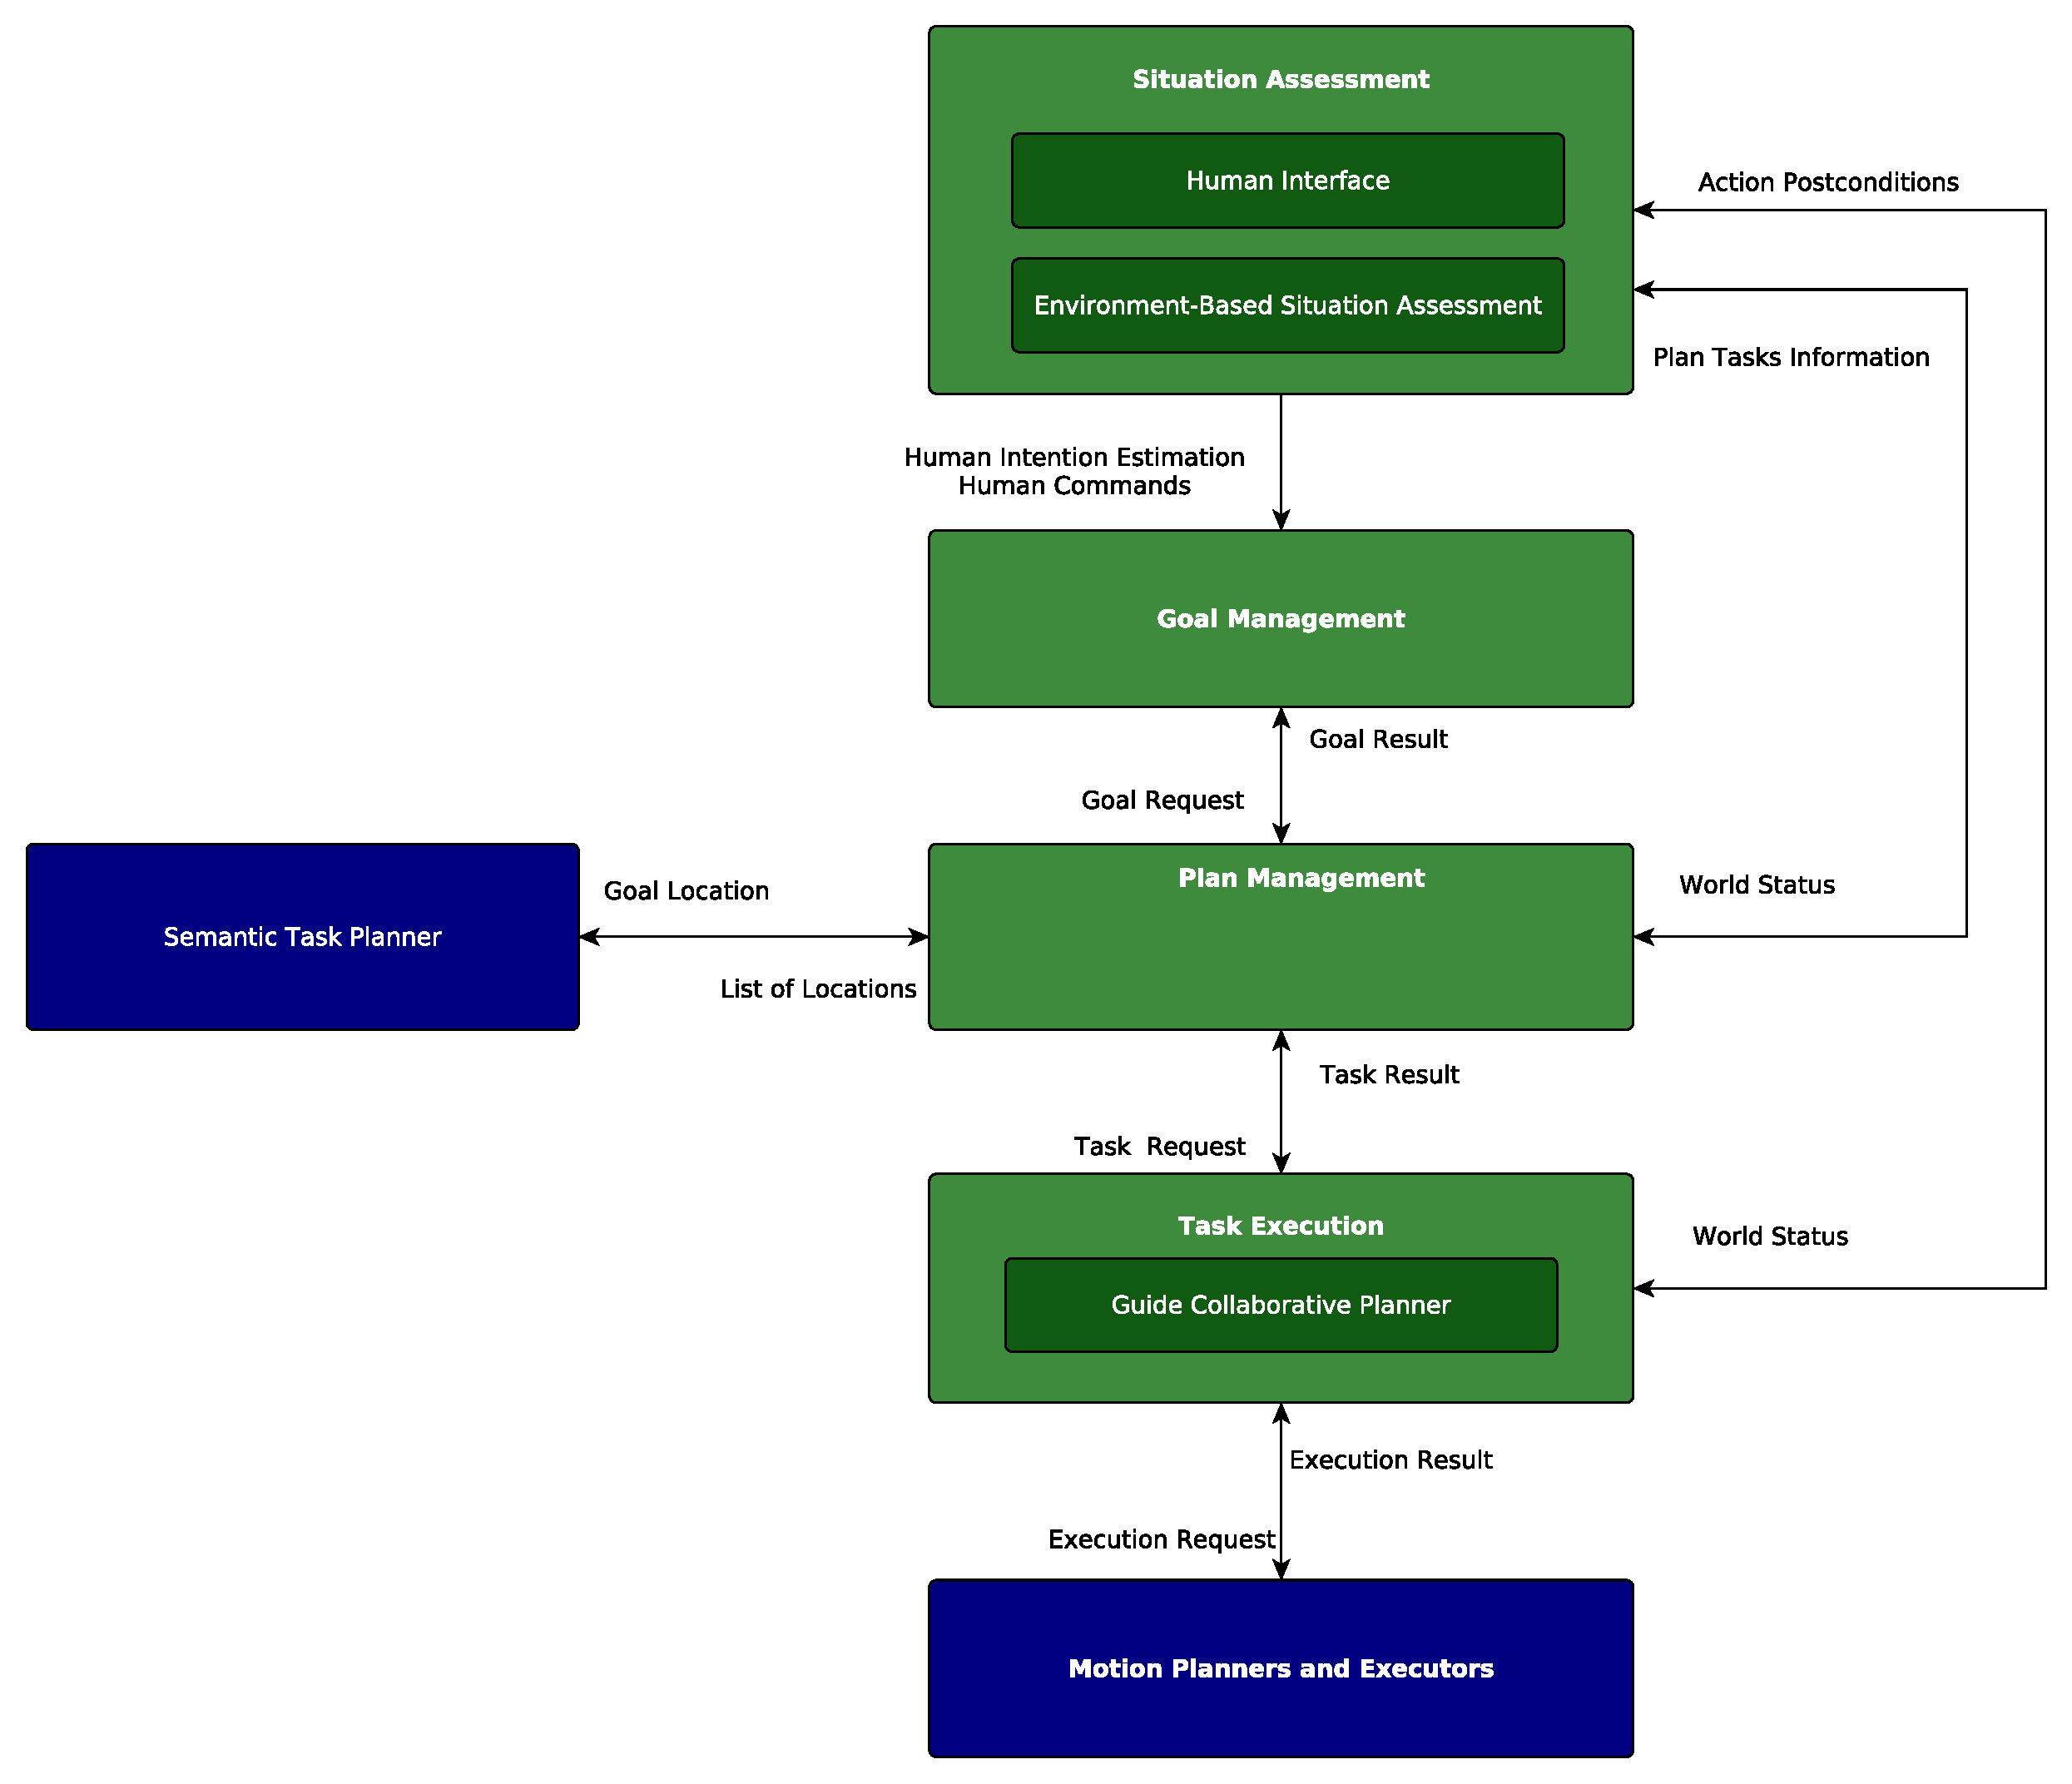
\includegraphics[scale=0.45]{img/case_study/spencer/architecture.pdf}
	\caption{This image shows the main layers of our architecture, as shown in \ref{intro-system_overview}. In each layer, represented as a light green rectangle, we show the modules that we modified or introduced in the robot guide scenario.}
	\label{fig:case_study-spencer-architecture}
\end{figure}

The system has been tested with different configurations, in laboratory experiments and in the Schipol airport, as shown in Subsection \ref{subsec:case_study-spencer-lab_exp} and \ref{subsec:case_study-spencer-airport}.

Parts of this work were presented in \cite{fiore2015adaptive}.

\subsection{Environment-Based Situation Assessment}
\label{subsec:case_study-spencer-intention}
There are many situations where, to properly reason on humans, we should link their movements and actions to the current environment. Imagine for example the case where we see a person oriented toward a screen. If an airport, we could infer from this observation that the person is looking at the screen, and perhaps in need of information. 

We introduced, in the Situation Assessment Layer, the ability able to create activity areas in the environment and link them to different kind of computations. An activity area is a polygonal or circular area, which can be fixed or linked and updated with an entity's (object, human or robot) position. We studied and experimented different two activity areas:

\begin{itemize}
\item Information Screen Area. This area, shown in Figure \ref{fig:case_study-spencer-screen_area} is linked to information screens present in the environment. Using this information, the robot can recognize that humans are looking at the screen, and  start a proactive behavior, like approaching to offering help or information.
\item Touristic Point Area, linked to interesting sights and attractions in the environment. We can imagine, for example, to link these areas to painting, statues, or even rooms in a museum. Knowing that a human is in a touristic point area, and looking at an attraction, the robot could approach the human and tell him some interesting information about it.
\end{itemize}

\begin{figure}[ht!]
	\centering
	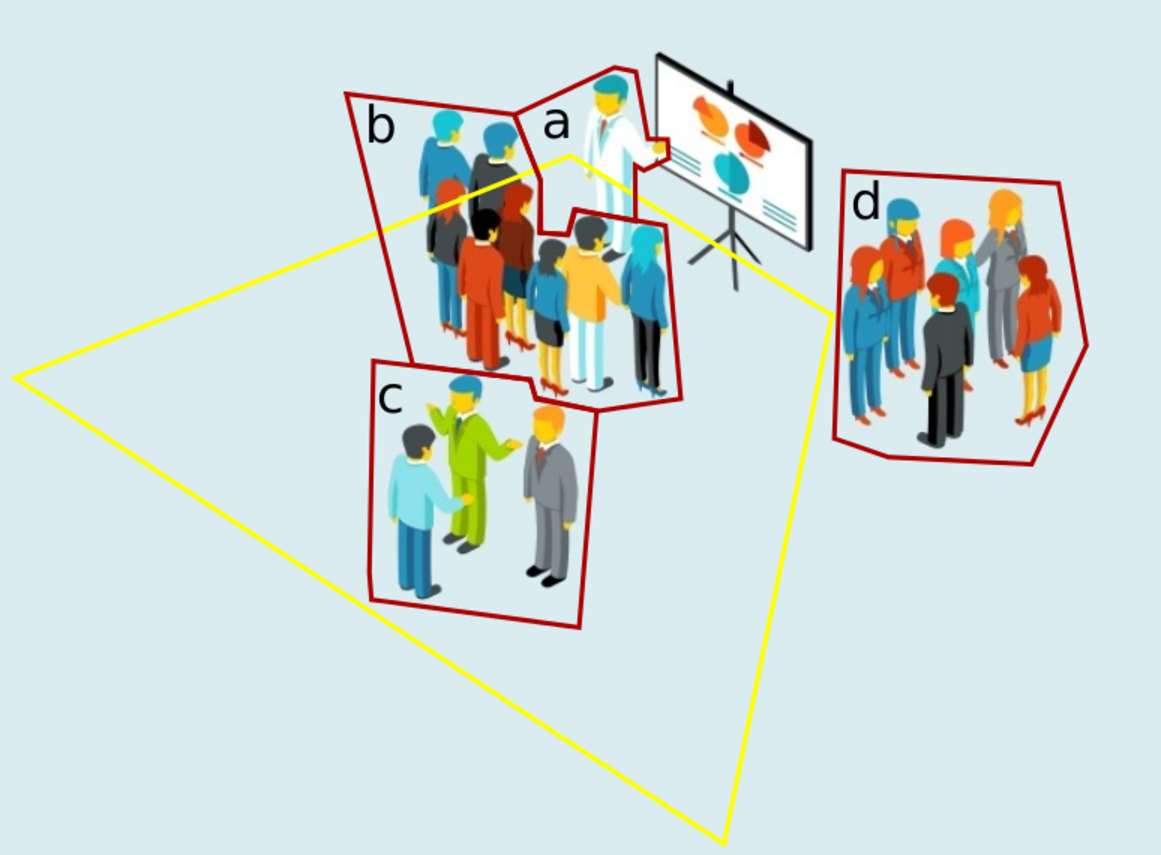
\includegraphics[scale=0.45]{img/case_study/spencer/environment_intention.pdf}
	\caption{This figure shows how the Information Screen Area used for environment-based intention recognition. The yellow polygon represents an area linked to the screen in the figure. Red polygons represent groups of person in the area. The person in group a is in the screen area, but the robot will infern that he is not looking at the screen, since he is oriented in another direction. The persons in group b are in the screen area and oriented toward the screen, so they are looking at it. The persons in group c are not looking at the screen since they are either oriented in another direction or outside its area.}
	\label{fig:case_study-spencer-screen_area}
\end{figure}


\subsection{Task and Motion Planning Problems}
\label{subsec:case_study-spencer-planning}
To guide people in environments like museum or airport, the robot will need to navigate very large areas, which are often too big to perform efficiently motion planning. A solution to this problem is reducing the size of the area where the motion planner will compute its paths, and splitting the navigation problem in a list of sub goals. The problem, with this approach,  is choosing the correct list of sub-goals to reach the final position.  To deal with this issue we implemented an A* based task planner, which will choose a high-level path to be followed by the robot from a semantic map. This map is a hand-crafted graph. composed by different nodes, representing parts of the environemt (corridor, elevator entrance, gates areas, etc.). Each node will be linked to a point in the real world. This task planner will, so, produce a list of coordinates usable by the motion planning layer. 

\begin{figure}[ht!]
	\centering
	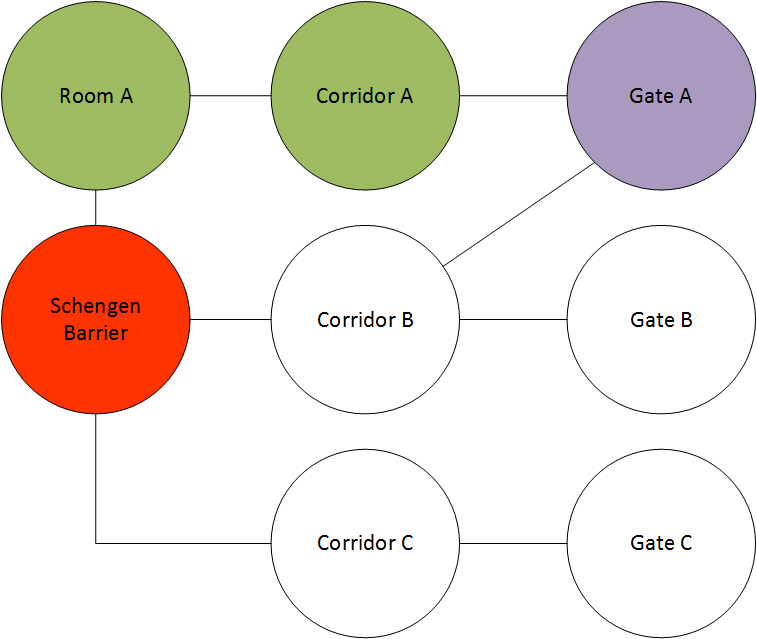
\includegraphics[scale=0.45]{img/case_study/spencer/ShengenTaskPlanner.png}
	\caption{This figure shows an example of plan computed in the spencer scenario. The circles represent nodes in the semantic map. The purle node is the starting node of the plan. The red node is the goal. The green node represent intermediate nodes in the plan.}
	\label{fig:case_study-spencer-semantic_plan}
\end{figure}


A first way to manage this kind of plan is simply travelling to each calculated point, sending a goal to the motion planner for the next point every time the robot reaches a node. The problem with this approach is that the path followed by the robot might be very inefficient and not look natural.

Our solution was using a rolling window approach, shown in Figure \ref{Fig:case_study-spencer-rolling_window} where the motion planner will plan on a grid map centered on the robot, which will move with it. In this way, the robot will send the next goal in the calculated plan as soon as it is present in the rolling window. It is very important, with this approach to carefully select the nodes in the semantic maps so that the rolling window will contain at least two semantic nodes. If not, the motion planner would have to plan a path to a goal outside its grid map, which would generate an error.


\begin{figure}[ht!]
	\centering
	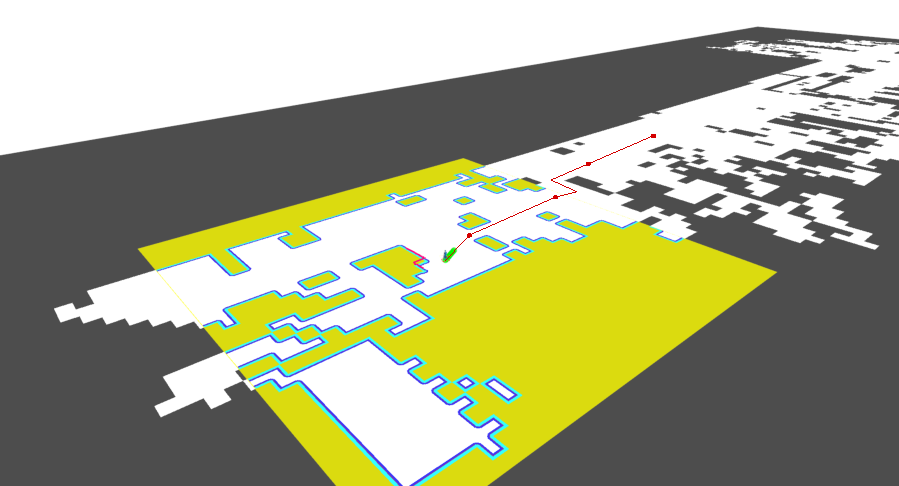
\includegraphics[scale=0.45]{img/case_study/spencer/rolling_window.pdf}
	\caption{This figure shows the rolling window approach. The motion planner will compute robot paths in the grid represented by the yellow area, which is always centered on the road. The red dots represent goals in the path, and are sent to the planner as soon as they are inside the window. The robot path does not pass through the closest node, since there is a further one in the rolling window.}
	\label{fig:case_study-spencer-team}
\end{figure}



\subsection{Collaborative Guide Planner }
\label{subsec:case_study-spencer-collaborative_guide_planner}

We developed a new collaborative planner to guide users to a destination. The planner is organized as hierarchic MOMDP, as shown in Figure \ref{fig:case_study-spencer-guide_planner} and is composed by several models:
\begin{itemize}
\item Guide Group Model. The main MOMDP of the hierarchy, responsible of choosing the main action performed by the robot.
\item Speed Adaptation Model. This model chooses if the robot should accelerate, decelerate, or keep the current speed.
\item Suspend Model. This module chooses which actions to execute when the group of followers has stopped following.
\end{itemize}



\begin{figure}[ht!]
	\centering
	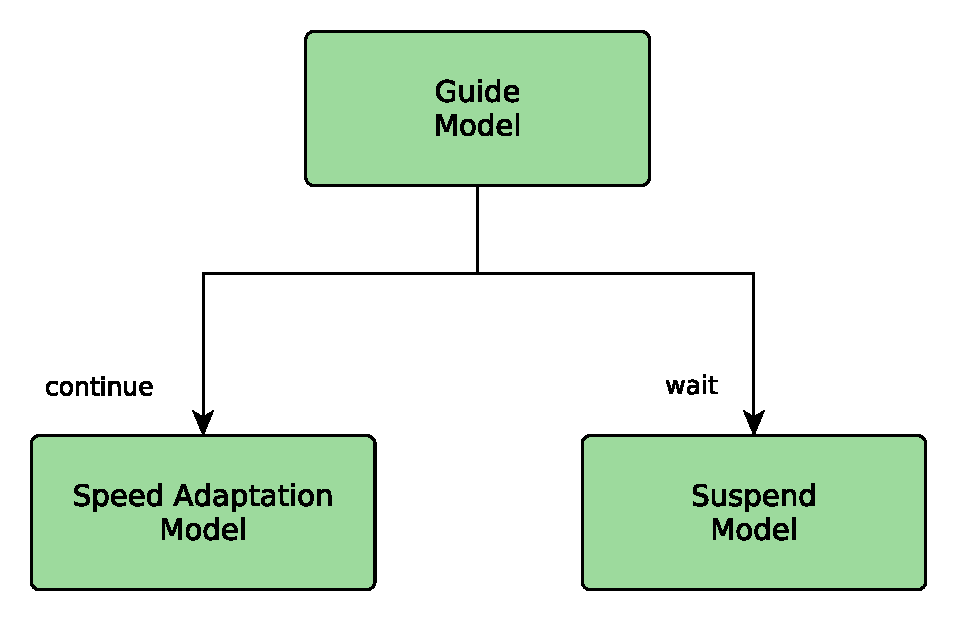
\includegraphics[scale=0.45]{img/case_study/spencer/guide_planner.pdf}
	\caption{This figure shows the hierarchical MOMDP collaborative planner use to guide a Group. The arrows show the macro-actions of the root of the hierarchy, leading to sub MOMDPs.}
	\label{fig:case_study-spencer-guide_planner}
\end{figure}

\subsection{Representing a group}
Our system has been built with the assumption that the robot would navigate in a crowded environment, where its followers could be often occluded. In addition, after speaking with our partners, we understood that the perception components would not be able to maintain a stable identifier for members of the groups, meaning that the robot would not be able to realiably understand if a group of users is following it. We tried to maintain a good balance between accuracy, trying to guide effective users and not people whose which are going in the same direction as the robot, and robustness, copying with unreliable perception.

We built our collaborative planner following these ideas:
\begin{itemize}
\item The robot will record a list $g$ composed by the identifiers of the group at the start of the scenario. During this scenario, it will maintain a list $f$, composed by users that are still tracked whose identifier is in $g$, and another list $o$, composed by all the tracked people whose distance from the robot is less than a costant $d$. 
\item As long as $f$ is not empty, the robot will choose a \textit{best} follower $b$ from this list, and try to guide him, using the collaborative planner. The \textit{best} follower is chosen by considering the user whose behavior is the most consistent with the robots, by taking into account the speed, the distance and the orientation of the user.
\item If $f$ is empty, but $o$ is not, the robot will choose a \textit{best} follower $b$ from $o$, and try to guide him, using the collaborative planners.
\item If  both $f$ and $o$ are empty, the robot will abandon the task.
\end{itemize}

Our idea is considering that the robot's followers will \textit{act as a group}, staying together as much as they can. The robot will try to guide members of the group, but if it has lost tracking to all of them, and there is still somebody behind it which is acting in a consistent way with the guiding task, it will think that its users are still following it, but their identifiers have changed in the perception layer.


\subsubsection{Guiding a User}
The main problem of the robot is choosing if it should still guide the group, suspend temporarily the task, or abandon it. The Guide Model is the main MOMDP of our architecture and will make this decision, based on three main variables: 
\begin{itemize}
\item The status of advancement of the task. This variables, whose values are ${not\_completed, completed}$, is set by the Action Executor module, in the Plan Execution Layer, depending on the current advancement of the task. The variable will be set as $not_completed$ until the robot as reached the final destination in the plan. 
\item The quality of commitment of the group. This variable, whose values are ${not\_engaged, engaged, not\_interested}$, is hidden, estimated from observations produced by the Situation Assessment Layer. The observations used are: the distance of the user from the robot, its variation, the orientation of the user in respect of the the robot, and if the user is currently moving or still. We expect engaged users to have a behavior that is coherent with the task, moving to follow the robot and taking a similar path. Users are considered not engaged when they stop following, perhaps even disappearing from the robot's sight. Finally, we infer that users are not interested in following the robot if they have stopped following for too long.
\item A timer. This variables can assume the values ${not\_expired, expired}$. When a user is detected as $not\_engaged$, the Action Executor starts a timer. When this timer expires, the value of this variable is set accordingly.
\end{itemize}

The Guide Model can execute the following actions:
\begin{itemize}
\item $Continue$. A macro-action, which leads to the Speed Adaptation Model.
\item $Wait$. A macro-action, which leads to the Suspend Model.
\item $Abandon$. Signals the Action Executor to abandon the current task.
\end{itemize}

\subsubsection{Adapting the Robot's Speed}
We believe that to be socially acceptable, the robot should adapt its speed to his follower. By setting its own pace at the start of the scenario the robot  would risk of being too slow, annoying users, or too fast, which would lead the robot to constantly stop to wait for users, producing an awkward behavior. Adapting to users might no be enough in some tasks, and depending on the situation, the robot might desire to influence the behavior of its group, to respect social rules or to accomplish its task in a more efficient way. Its important to find a balance between these two behaviors, which is the goal of the Speed Adaptation Module. 

To adapt to the speed of the group, the robot defines a desired range of distances $[dr_1,dr_2]$ from the best follower $b$. The distance of $b$ from the robot, $d(b,r)$ will influence the chosen action:
\begin{itemize}
\item if $d(b,r)>dr_2$ the robot will influence the robot to \textit{decelerate}.
\item if $d(b,r)<dr_1$ the robot will influence the robot to \textit{accelerate}.
\item if $dr_1<d(b,r)<dr_2$ the robot will influence the robot to maintain its current speed.
\end{itemize} 

In our study, $dr_1$ and $dr_2$ were predefined values, but they could be learnt and adapted to the users during the task, since different people could prefer following the robot at different distances and positions.

The robot should also not constantly change speed, in order to give time to users to adapt to its new chosen speed, and so we defined a temporal threshold in which we do not allow the robot to repeat an \textit{accelerate} or \textit{decelerate} action.

We studied two different situations where the robot can proactively try to influence the speed of the group.
\begin{itemize}
\item There is a time limit to reach the destination. In this case the robot must balance the desire to satisfy the group with the task urgency. Different situations will require different policies. For example, in an airport scenario, the robot could prioritize arriving on time, warning users if their speed would render the goal not achievable, while in other situations the robot could try to arrive in time but still avoid to adopt speeds that are uncomfortable for the group.
\item The rules of the current environment limit the robot's speed. In this case the robot will avoid accelerating over a set speed even if it detects that its current velocity is considered too slow for the group. For example, the robot could be navigating in a construction zone.
\end{itemize}

\subsubsection{Suspending the task}
In some situation, the robot needs to suspend the task, because the group has stopped following it. In this case, the robot should estimate if this suspension of the collaborative scenario is temporary or permanent, and in the latter case abandon the task. We estimate this information using the Suspend Model and the activity areas from Situation Assessment. We link activity areas to the maximum time we expect that the group will be involved in the linked activity, and with a set of proactive actions that the robot can choose to execute.

In our work, we investigated a single possible proactive behavior: giving information. In this case, if we detect that one or more  members
of the group has stopped following because it is looking at a touristic sight, or at an information screen, the robot can try to engage him and offer related information. At the moment, we just propose a simple routine-based framework for this behavior, and plan to further study it in the future. We believe that the solution of this problem could be rich, and that the robot should estimate the reaction of the group during the execution of its proactive behavior, in order to be able to interrupt if the group does not want to be helped or to resume the original task if they are satisfied by the robot's actions.

We do not want the robot to be inactive for a long time  waiting for the group. If there is a small amount of time to reach the destination, or the group is engaged in the activity for a longer period of time than the one predicted, or the robot can not estimate the reason why the group stopped following, the Suspend Model can issue a warning action, and eventually abandon the task if the group does not start following it again.

\subsection{Laboratory Experiments and Analysis}
To have a first validation of our system, we performed experiments in a laboratory.

In this setting, we used Motion Capture to track users, and a navigation software based on \cite{sisbotTRO2007,kruse12crossing}, which add proxemics based costs to static humans in the environment, and continuously predicts and avoid future collisions with moving persons,  simultaneously keeping the robot as close as possible on the planned path.

\begin{figure}[ht!]
	\centering
	\includegraphics[scale=0.2]{img/case_study/spencer/robotGuiding.png}
	\caption{This figure shows the SPENCER robot guiding a user in a laboratory}
	\label{fig:case_study-spencer-robotGuiding}
\end{figure}

We performed experiments with a single user following a robot on a predefined path. Data from these experiments are shown in Table \ref{table:case-study-spencer-experiment_results}. We start by showing speed adaptation tests:
\begin{itemize}
\item adapting slow and fast. In these two tests (Figure \ref{fig:case_study-spencer-robotGuiding}) we used our system to guide respectively a user that would like to move at a slow pace, and a user that would like to move at a fast speed.
\item no adaptation: in this experiments the robot will not adapt to the speed of the user, setting its own pace and stopping if it is too far.
\end{itemize}

Looking at the data we can see that our system shows lower values for the variance of speed and distance, which means that after a certain time it is able to find a condition of equilibrium with the human follower. The 'no adaptation' system shows a significantly higher variance for both values, since the robot stopped several times to wait for a user. We will now show some tests regarding the proactive behaviors of the robot:

\begin{itemize}
\item proactive slow and fast: during the task, the robot proactively chooses to change pace, in the first case by slowing down and in the second by accelerating. In our tests the user adapted after some seconds to the robot's pace, but this behaviors should be studied in-depth in user studies.
\item suspend with screen and with no reason: in these tests we asked a user to stop during the task. In the first case the user stopped near an information screen. After detecting this event, the robot approached the user to offer information, which lead to the resumption of the task. In the second case the user stopped at a different point of the path. The robot was not able to detect the reason for the suspension of the task and so simply   issued a warning to the user, abandoning the task after some seconds.
\end{itemize}


\begin{table}
\caption{Experiment results: $d$ is the distance between the robot and the user, $s_r$ is the robot's speed, $s_h$ is the human's speed, $\mu$ is the average and $\Delta$ is the variation of the quantity. Distances are expressed in meters, velocities in meters for seconds.}
\centering
\begin{tabular}{ | c | c | c | c | c | }

\hline
  test name     & $\mu$ $distance$ & $\mu$ $speed$ $difference$ & $\Delta$ $distance$ & $\Delta$ $speed$ $difference$ \\
\hline
adapting slow & 2.82 & -0.03 & 0.64 & 0.02 \\
  \hline
  adapting fast & 1.38 & 0.00 & 0.29 & 0.01 \\
  \hline
  no adaptation & 3.08 & -0.09 & 1.04 & 0.07 \\
\hline
proactive slow & 1.45 & -0.06 & 0.04 & 0.10 \\
\hline
proactive fast & 2.66 & -0.11 & 0.63 & 0.01 \\
\hline
\end{tabular}
\label{table:case-study-spencer-experiment_results}
\end{table}


\subsection{Results on Airport Deployment}
\label{subsec:case_study-spencer-airport}
\subsubsection{Integration with Other Components}
The system was deployed in the Schiphol Airport for two different sessions, respectively of a week and of two weeks. In those weeks the team of the SPENCER project adapted the robot to the complex environment of the airport. Our system was integrated with several softwares from our partners, such as a combined laser-RGB people tracker, developed in \cite{lindermulti}, a novel localization approach, as shown in \cite{kucner2015ndt}, an RTT based motion planner, shown in \cite{palmierirrt}, and cost-based social rules, shown in \cite{okallearning}. More details on the whole SPENCER system are available in \cite{triebel2015spencer}.


\begin{figure}[ht!]
	\centering
	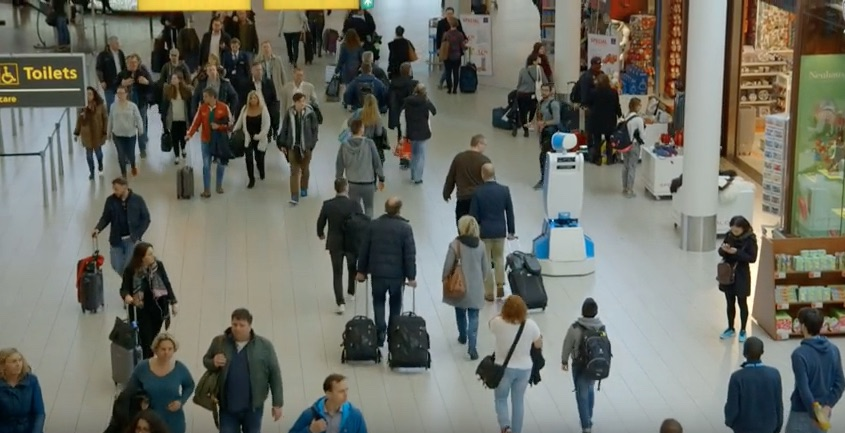
\includegraphics[scale=0.45]{img/case_study/spencer/spencer_schiphol.png}
	\caption{This figure shows the robot moving in the Schipol airport}
	\label{fig:case_study-spencer-spencer_moving}
\end{figure}


\begin{figure}[ht!]
	\centering
	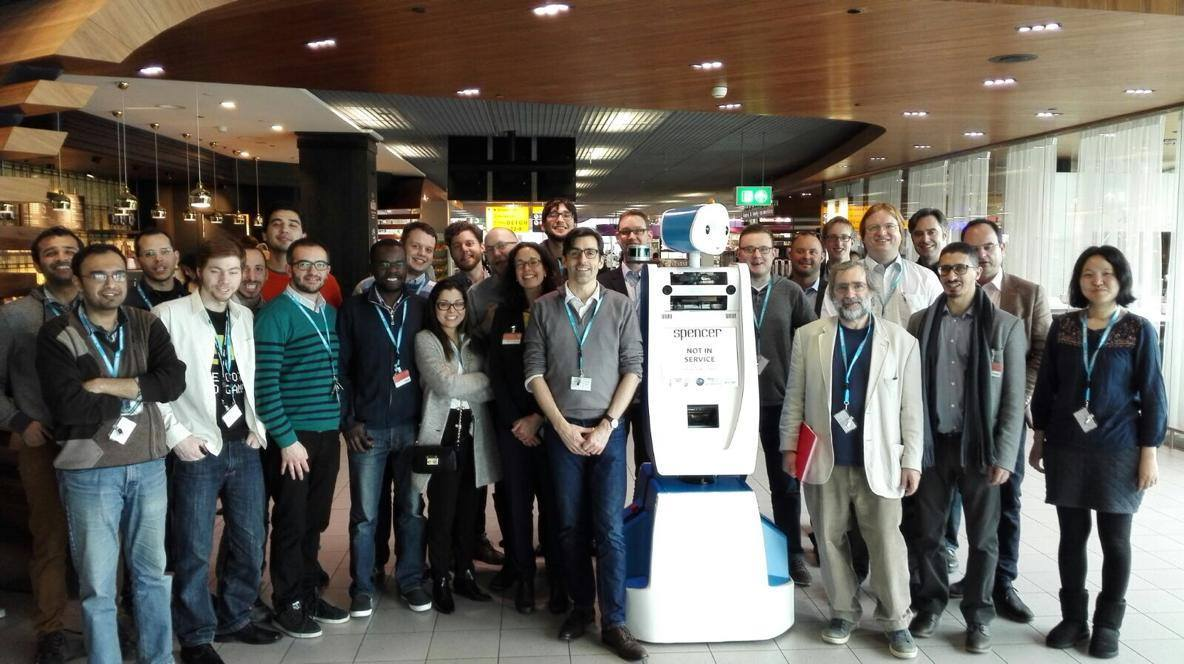
\includegraphics[scale=0.45]{img/case_study/spencer/all.jpg}
	\caption{This figure shows the team that worked on the SPENCER project.}
	\label{fig:case_study-spencer-team}
\end{figure}

\subsubsection{User Study}

The system was tested in an user study, performed by researchers of the University of Twente\footnote{https://www.utwente.nl/en/}, which participated in the project. The study was conducted in two different days, with 18 participants, 11 males and 7 females, aged between 26 and 54. Ten participants indicated that the purpose of their journey was business, while eight indicated pleasure. Two different tests were performed:

\begin{itemize} 
\item In the first test the robot would pick up users at a chosen point, in Lounge-1 or in the Starbucks coffee shop of the airport, and guide them to a prefixed gate, B18. Users interacted with the robot by scanning special boarding passes created for this test on the robot's board pass reader, which prompted the start of the mission. To reach the gate, the robot had to pass through a crowded area, composed by several shops and other flight gates.
\item In the second test the robot met users at the gate B18 and guided them to Lounge-1. In this situation users initiated the mission by using the touchscreen display of the robot to select the destination.
\end{itemize}

At the end of each test, we collected three different kind of measures:
\begin{enumerate}
\item An individual feedback questionnaire where the user evaluated several aspects of the robot, like its behavior and aspect, on a 7-point Likert scale. In the day of testing two new questions where introduced about the robot, and a question on the participant's opinion on the robot in general.
\item A group interview, where users could discuss about their first impression of the robot, their experience in the test, and their thoughts on how to improve the systemm.
\item  Notes taken by researchers during guide, that helped to contextualize the results of users and to record specifc events that occurred during tests.
\end{enumerate}


\begin{figure}[tb]
  \begin{center}
  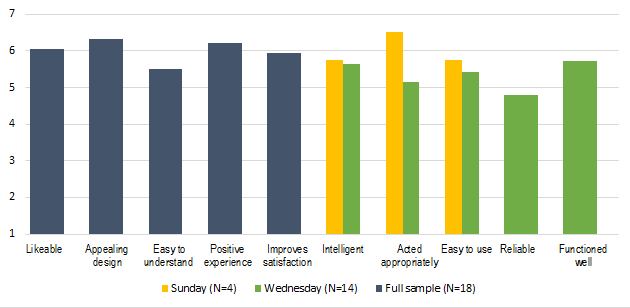
\includegraphics[width=0.95\textwidth]{img/case_study/spencer/graph_subjective_questions.png}
  \end{center}
  \caption{Answers to feedback questionnaire}
  \label{fig:feedback_questionnaire}
\end{figure}


Figure \ref{fig:feedback_questionnaire} shows the results of the feedback questionnaire. Two questions were reformulated between the two days of testing, and so we included means for both questions. While the number of tests conducted where too limited to generalize, we can affirm, that the participants had in general a positive impression of the robot. We list the main results of this test.

\begin{itemize}
\item Participants were generally happy with the robot's guiding performance.
\item The robot can be described as friendly-looking, easy-to-use and reliable.
\item The main issues encountered by users where related to the boarding card reader of the robot, and to its frequent abrupt stoppings.
\item Some users considered the speed of the robot too fast, or too slow, for their experience.
\item Users thought that the robot guide could be useful for people inexperience with flying, or new to a particular airport.
\item Users thought that the robot improved their customer satisfaction.
\item Main improvements for the robot include technical improvements, in particular related to the frequent stopping, and the addition of new functionalities, like carrying luggage or guiding to shops and restrooms.
\end{itemize}

\subsubsection{Discussion}
The experience in the airport showed the complexity of deploying a robot in such a complex scenario, interacting with inexperienced users. From our experiments we noticed several things:
\begin{itemize}
\item It is important to not make too many assumption about how users will interact with the robot. We expected users to follow the robot, staying mostly on its rear or side regions. This was not always true. In fact, several users where more interested in moving ahead of the robot, often concentrating on its behaviors more than on following it. The robot should adapt to these behaviors and not consider them as errors.
\item Human-Aware motion in complex environments is still a complex subject. Adapting the robot speed was not simple, because the robot had stop or slow down often to avoid obstacles. Some times false positives generated by perception can lead to abrupt stop by the robot, which are seen as annoying and innatural by users, and could even be dangerous.
\item Users are fascinated by robots, and are willing to ignore errors generated by the systems in short-term experiences.
\item It is important to perform long deployments in similar scenarios with real users. A long time in the three weeks where we worked at the airport was spent adapting the robot to the scenario. Longer deployments would allow for an iterative process of design-implementation-study.
\end{itemize}


\section{Robot Helper}
\subsection{Introduction}
In this section we show experiments created to validate our system in a domestic scenario, where the robot can help a human partner to achieve a joint task. Parts of this section where presented in \cite{fioreiser2014}.

\subsection{Experiment Description}
We present a scenario where the robot and a human have a joint goal: cleaning a set of furniture. 
The environment is composed by two different furniture, $TABLE\_4$ and $IKEA\_SHELF$, and three tapes,
 $GREY\_TAPE$, $LOTR\_TAPE$ and $WALLE\_TAPE$. The goal of the agents is throwing each tape in a bin,
 $PINK\_TRASHBIN$. We will present different examples, where the items will be placed differently, depending on our needs. The scenario is shown in Figure \ref{fig:case_study-helper-pr2helper}

 \begin{figure}[ht!]
 	\centering
 	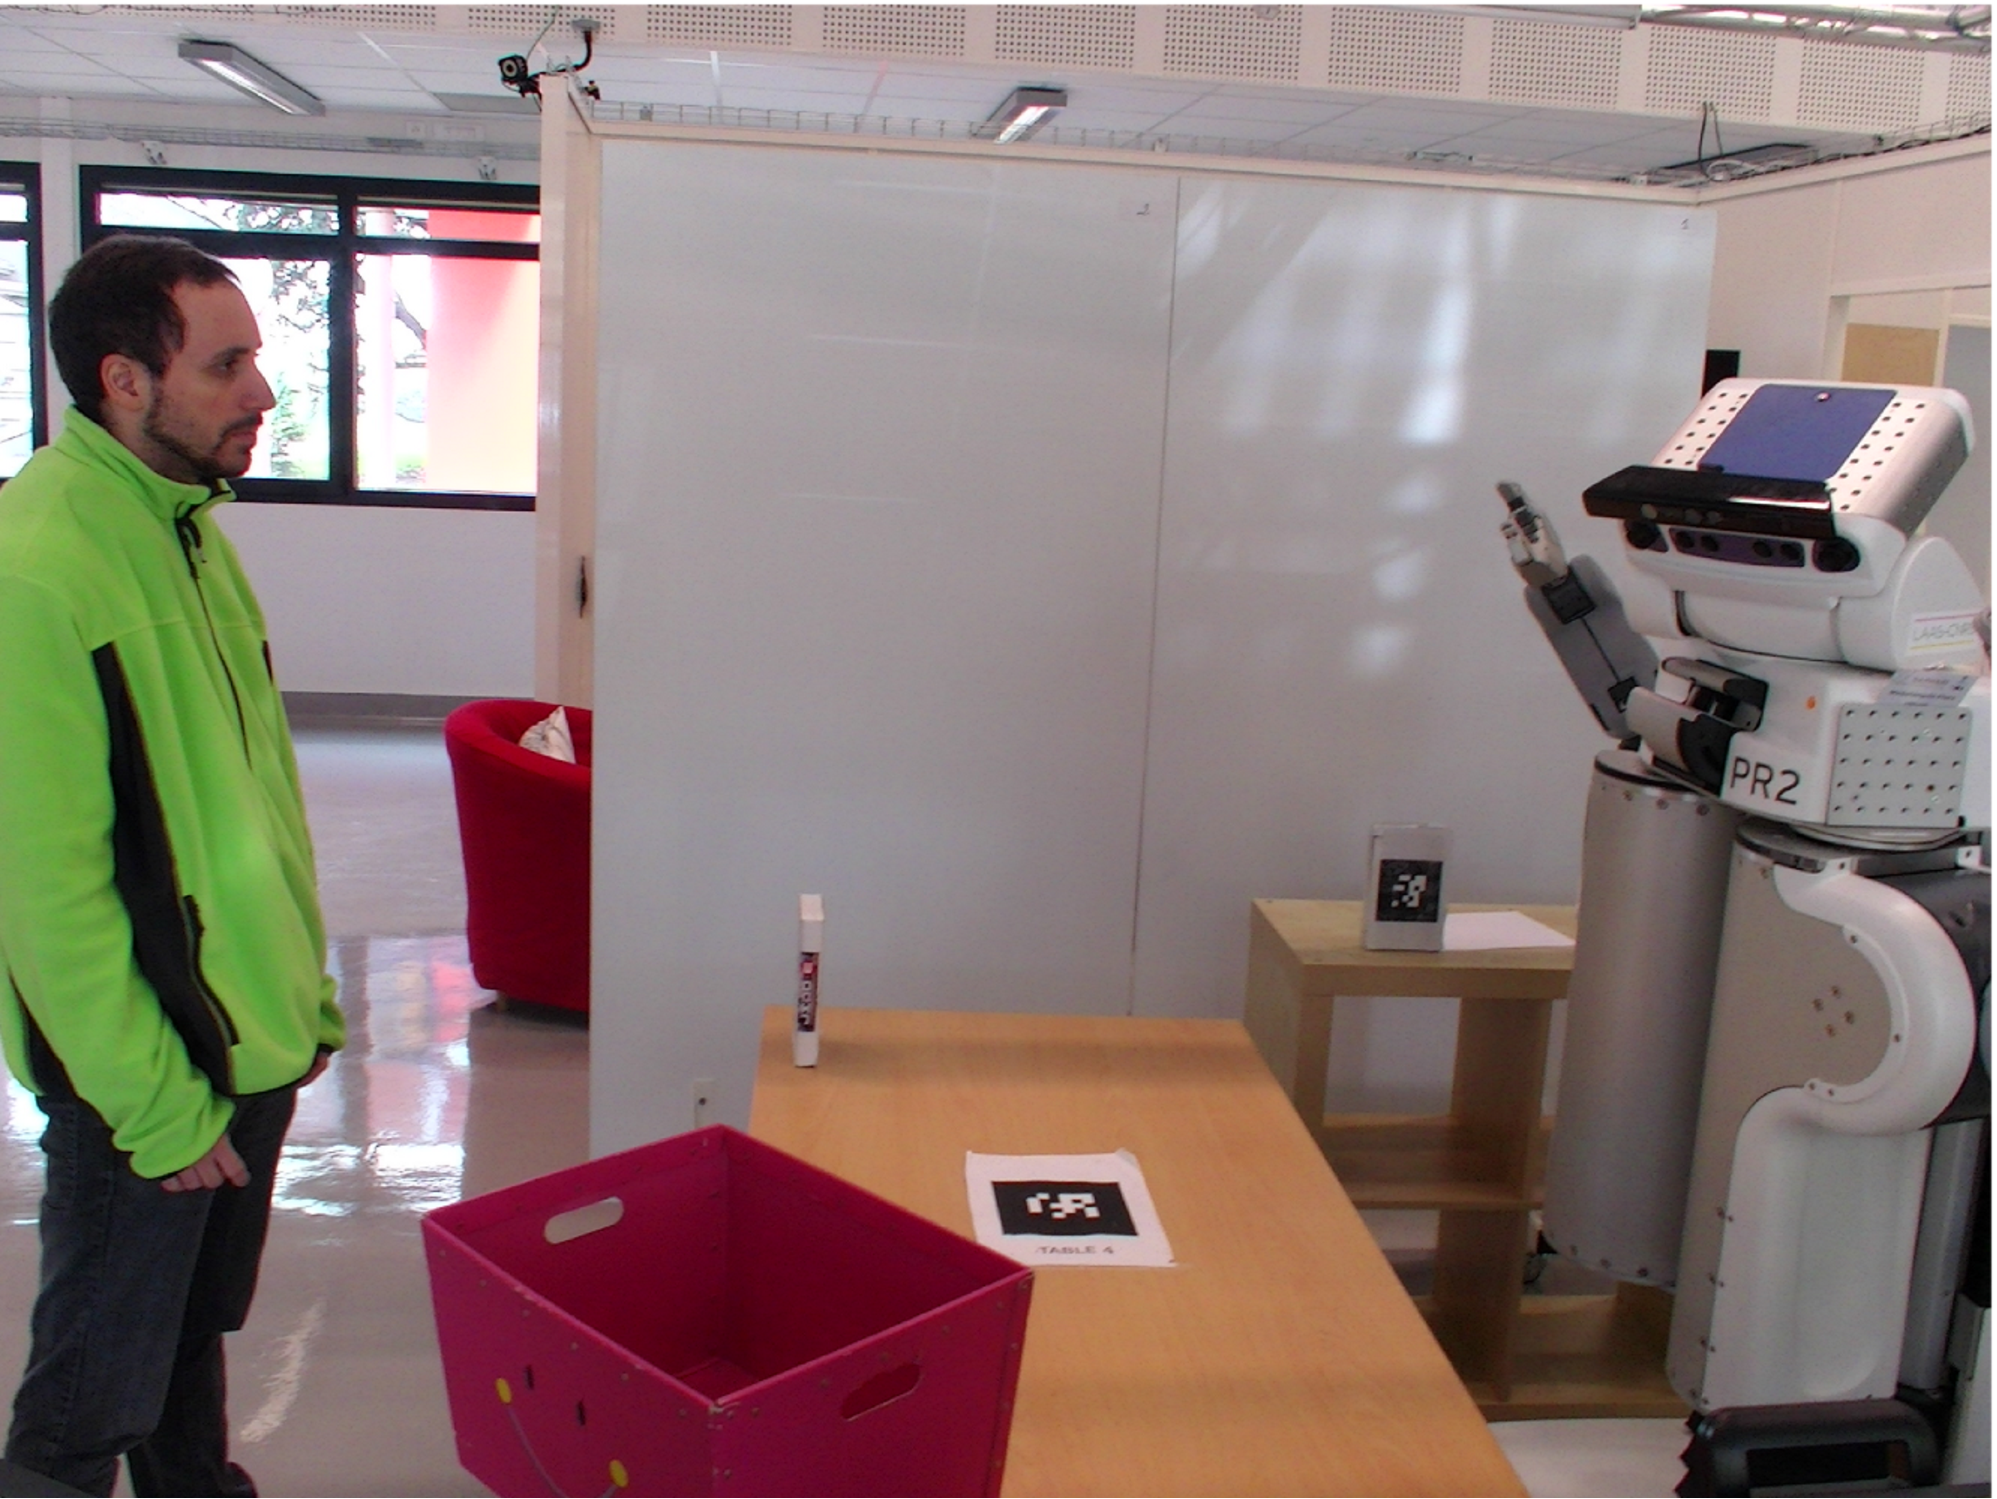
\includegraphics[scale=0.45]{img/case_study/helper/experiment.pdf}
 	\caption{This figure shows the robot helper scenario, with a PR2 robot and a user.}
 	\label{fig:case_study-helper-pr2helper}
 \end{figure}

For this scenario, we used a previous version of the system described in the previous chapters, with the addition of the Handover Collaboration Planner, used to execute human-robot and robot-human handovers. In particular, in this version, the robot does not take into account the knowledge level of users when producing or managing plans. Also, human tracking will be done using a depth camera, mounted on the ceiling.

\subsection{Handover Collaboration Planner}

We implemented an MOMDP model to handle handovers between humans and robots. This model will output high-level actions, adapted by the Action Executor, depending on the current situation. Decisisions will be made based on the following variables:

\begin{itemize}
\item The status of advancement of the task. This variables, whose values are ${not\_completed, touching, completed}$, is set by the Action Executor module, in the Plan Execution Layer, depending on the current advancement of the task. The variable will be set as $completed$ when the handover has been performed, $touching$ when the robot detects pressure on the gripper used for the handover, and $not_completed$ otherwise. 
\item The quality of commitment of the user. This variable has the same meaning as in the collaborative planner for guiding presented in \ref{subsec:case_study-spencer-collaborative_guide_planner} and can assume the same values, but is estimated from different variables. We will still consider the distance and orientation of the human toward the robot, but also the pose of its arm, particularly if its extended toward the robot. 
\item A timer. The variable is used in the same way as in the collaborative planner for guiding presented in \ref{subsec:case_study-spencer-collaborative_guide_planner}.
\end{itemize}

The possible actions of this model are the following:
\begin{itemize}
\item Continue. The Action Executor will continue with the handover, which depending on the situation, will prompt the system to extend the arm or activate the gripper.
\item Wait. The system will wait for the user. if it is not engaged in the task.
\item Abandon. The system will abandon the task when the user is no longer interested in performing it. 
\end{itemize} 


\begin{itemize}
  \item
\textbf{Equal Partners}:
In this scenario (figure \ref{fig:case_study-helper-scenario1}) the user is asked to clean the table, without explaining him what is shared plan that will be used. The user is just informed that
the robot will try to help as it can to perform the task. The user moves to the table and
takes the $WALLE\_TAPE$. At this point, the robot notices that the user
has completed an action and understands that he wants to clean the
table.
\begin{figure}
  \caption{Robot adapts.This figure shows the robot's representation of the scenario. The white tape is the WALLE\_TAPE, while the blue
    one is the LOTR\_TAPE. The round shapes represent the agents'
    rechabilities, with red shapes representing robot reachabilities
    and green shapes human reachabilities. In this case only the human
  can reach the WALLE\_TAPE while both agents can reach the LOTR\_TAPE
and the PINK\_TRASHBIN. After the human takes the WALLE\_TAPE the
robot produces a plan where the human must throw the tape in the
bin while the robot can take the LOTR\_TAPE and throw it in the
bin.
}
\centering
  \subfigure{
  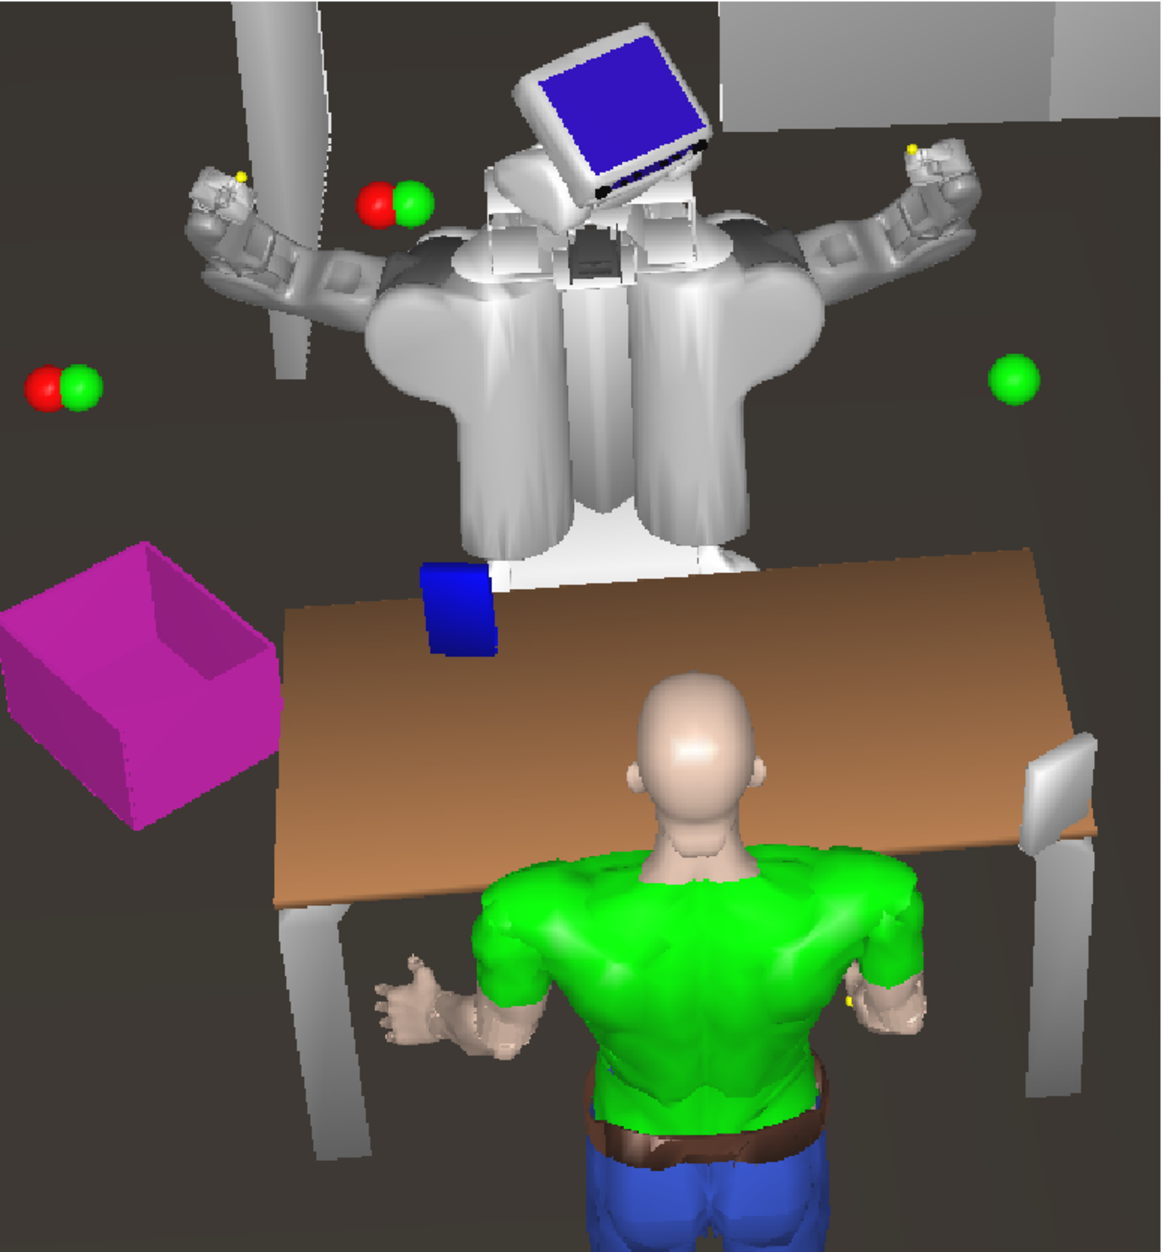
\includegraphics[scale=0.25]{img/case_study/helper/scenario1.pdf}
  }
  \subfigure{
  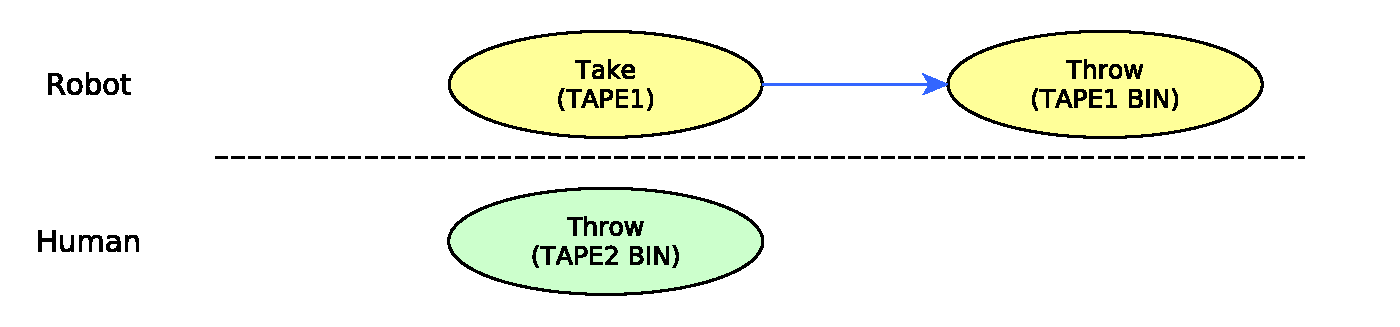
\includegraphics[scale=0.7]{img/case_study/helper/plan1.pdf}
  }
  \label{fig:case_study-helper-scenario1}
\end{figure}

The robot creates a plan and executes its part of it while monitoring the human,
which executes its part without deviating from the plan calculated by
the robot.

\item
\textbf{Modality switch and user plans}:
In this scenario (figure \ref{fig:case_study-helper_scenario2}) the robot is the only agent able to reach both tapes, but it can not reach
the bin, which can instead be reached by the human. We tested
this scenario in two different runs. In the first run, the current plan management modality is 'Robot Leader'.
After exploring the environment, the robot produces a plan and starts its execution.

\begin{figure}
  \centering
  \caption{Modality switch and user plans. Another configuration of
    the environment, where the robot can reach the two tapes and the
    human can reach the thrashbin. The robot generates an initial plan
  from this situation. The block surrounding the Give and Receive
  actions means that they are considered a single joint action.}
  \centering
  \subfigure {
    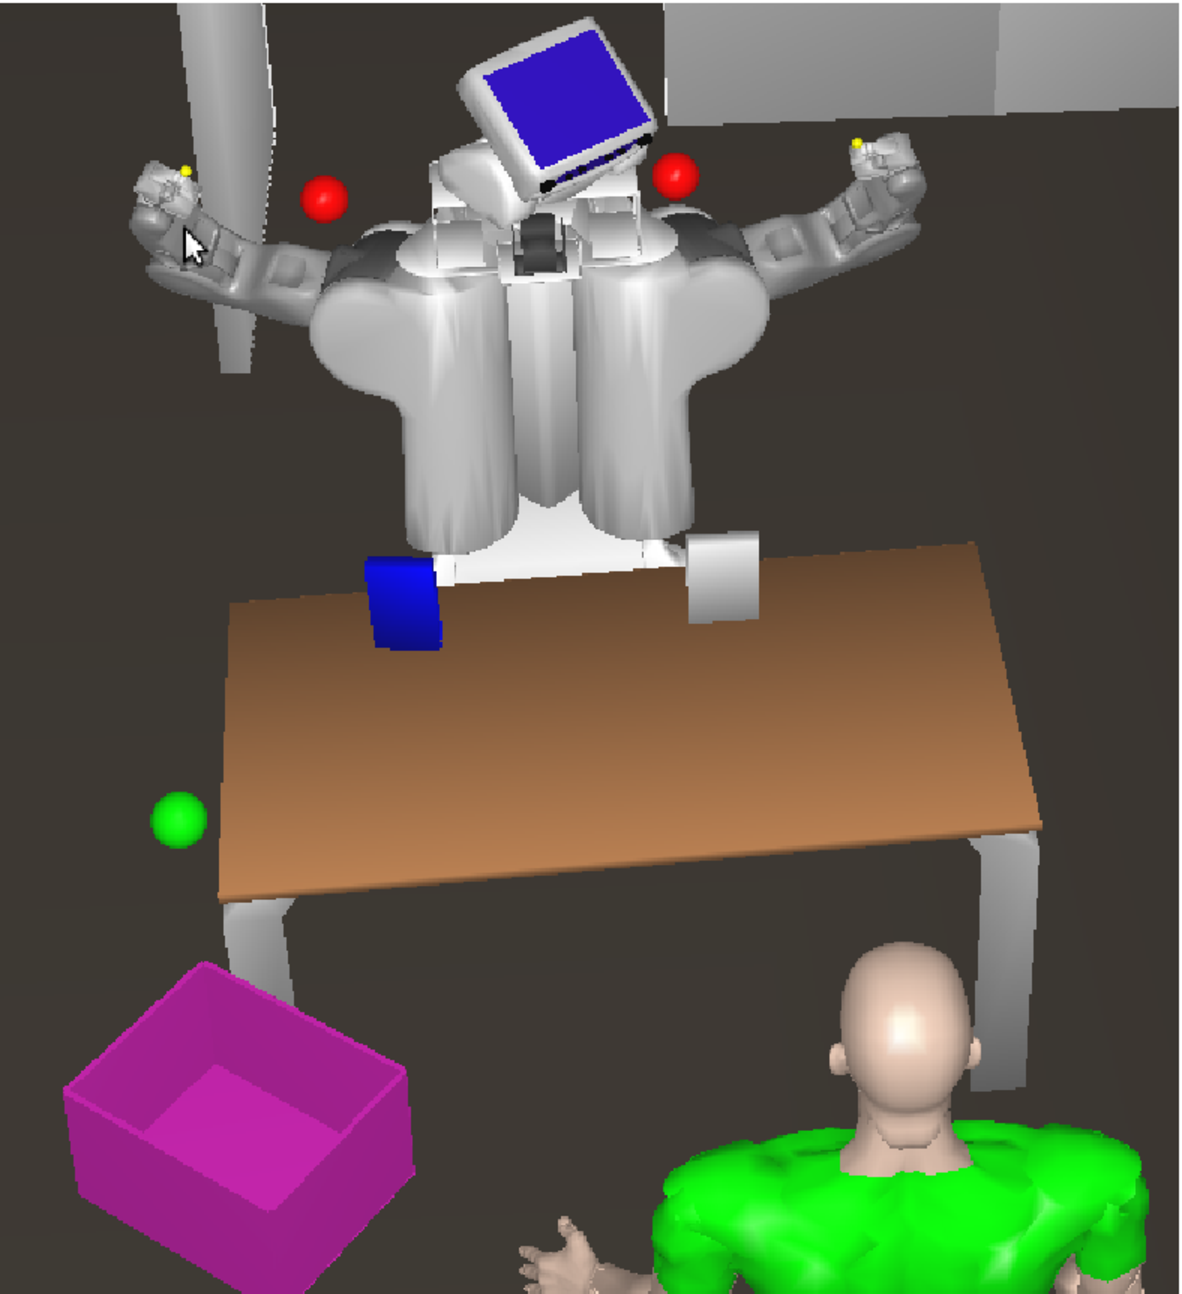
\includegraphics[scale=0.25]{img/case_study/helper/scenario2.pdf}
   }
  \subfigure {
    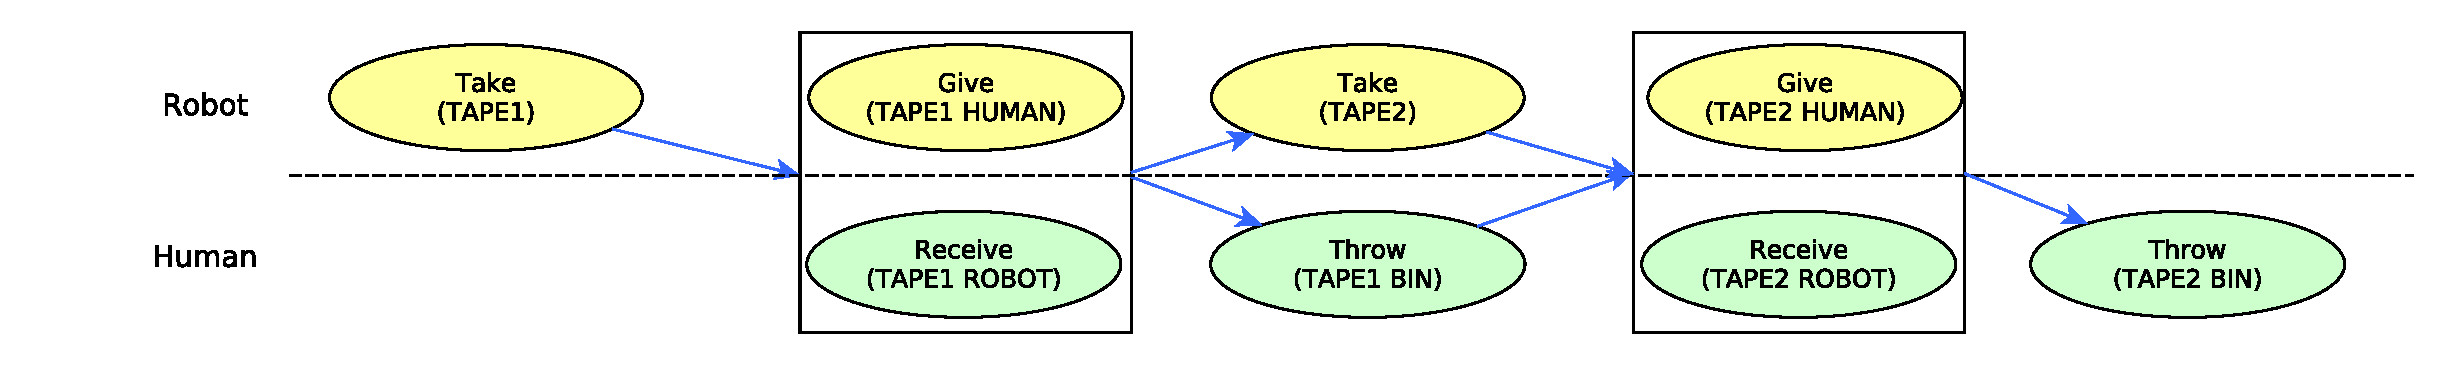
\includegraphics[scale=0.4]{img/case_study/helper/plan2.pdf}
  }
  \label{fig:case_study-helper_scenario2}
\end{figure}

While the robot is taking the $LOTR\_TAPE$ the human moves
to take the $WALLE\_TAPE$. This deviates from the robot plan, so it
switches to the 'equal partners' modality, communicating the change to
the user. The user throws the $WALLE\_TAPE$ in the $PINK\_TRASHBIN$ while
the robot takes the $LOTR\_TAPE$ and handles it to the user. The user
takes the $LOTR\_TAPE$ and throws it in the $PINK\_TRASHBIN$, completing the task.

In the second run the current modality is'Human Leader' mode. The user is
asked to clean the table as he wishes. The user asks the robot to take
each tape and give it to him, throwing them in the trashbin.

\item
\textbf{Replanning after failed action}: 
In this scenario (figure \ref{fig:case_study-helper-scenario3}) the robot is the only agent able to reach the
bin, while both agents can reach the two tapes. The
robot is in 'Robot Leader' modality and, after examining the
environment, produces a plan.

\begin{figure}
  \caption{Replanning after failed action. Here we can see a first
    plan, produced at the start of the scenario, and a second,
    produced after the robot fails to take the WALLE\_TAPE. }
  \centering
  \subfigure{
    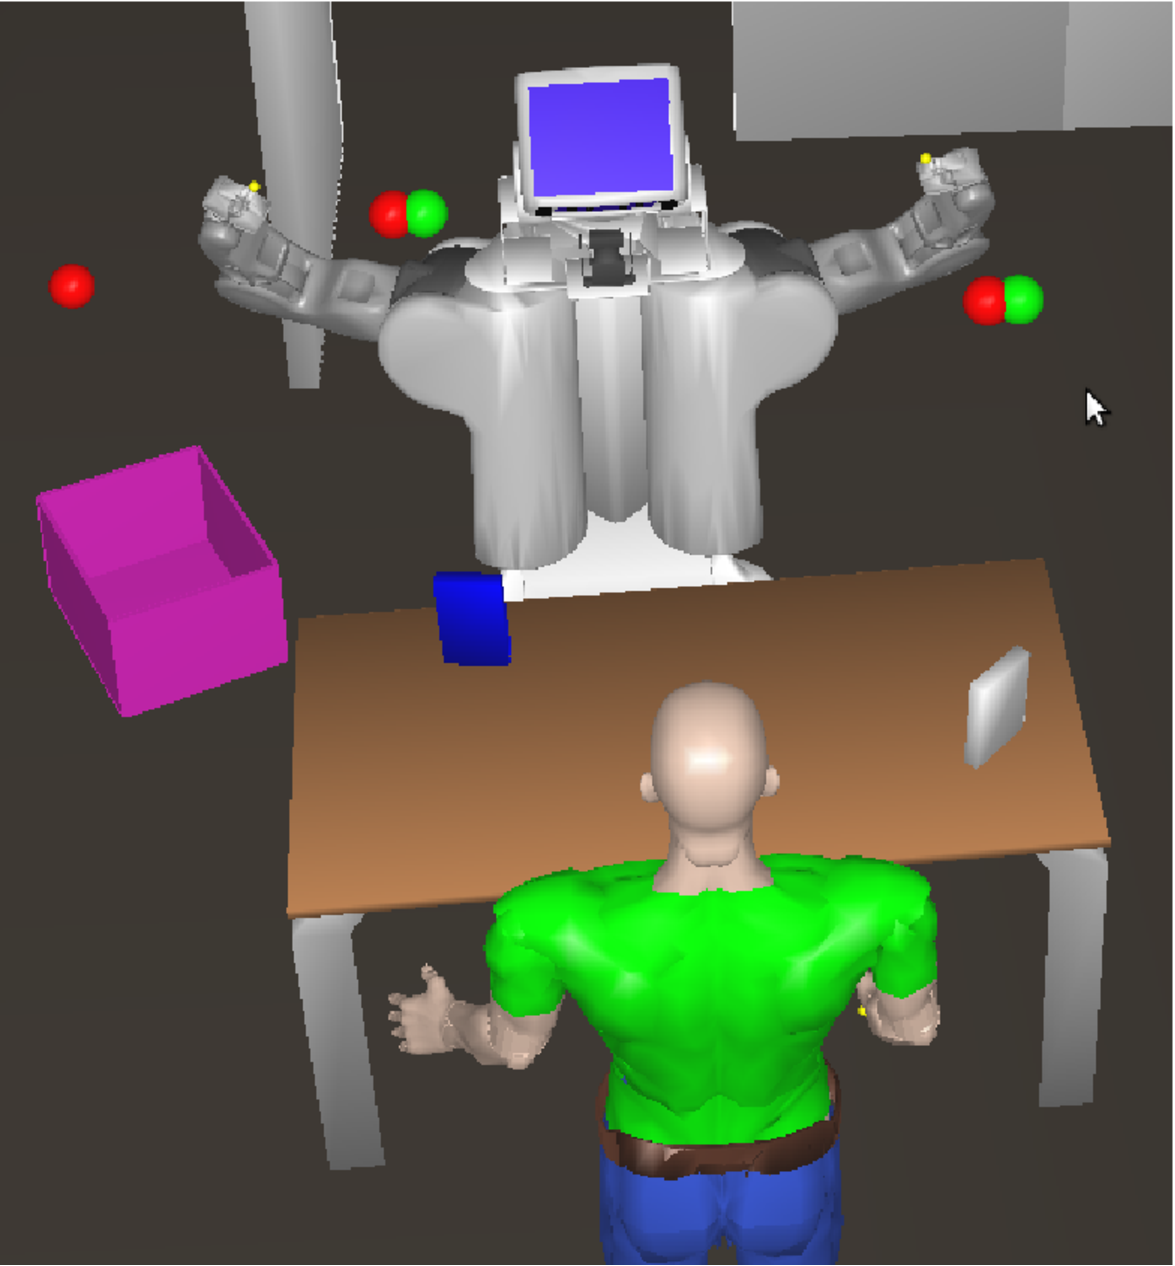
\includegraphics[scale=0.25]{img/case_study/helper/scenario3.pdf}
    }
    \subfigure {
      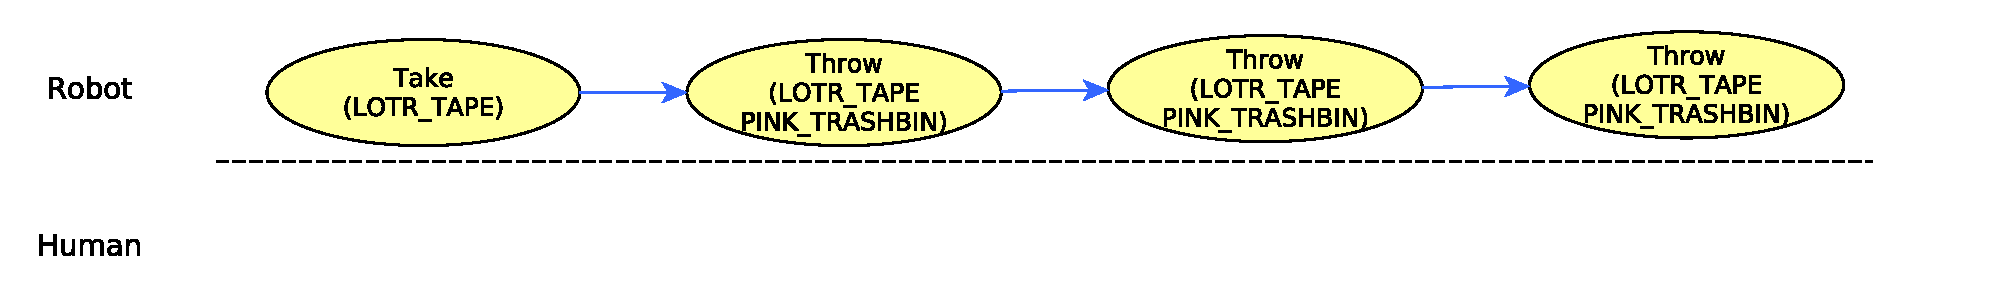
\includegraphics[scale=0.5]{img/case_study/helper/plan3.pdf}

      }
      \subfigure {
        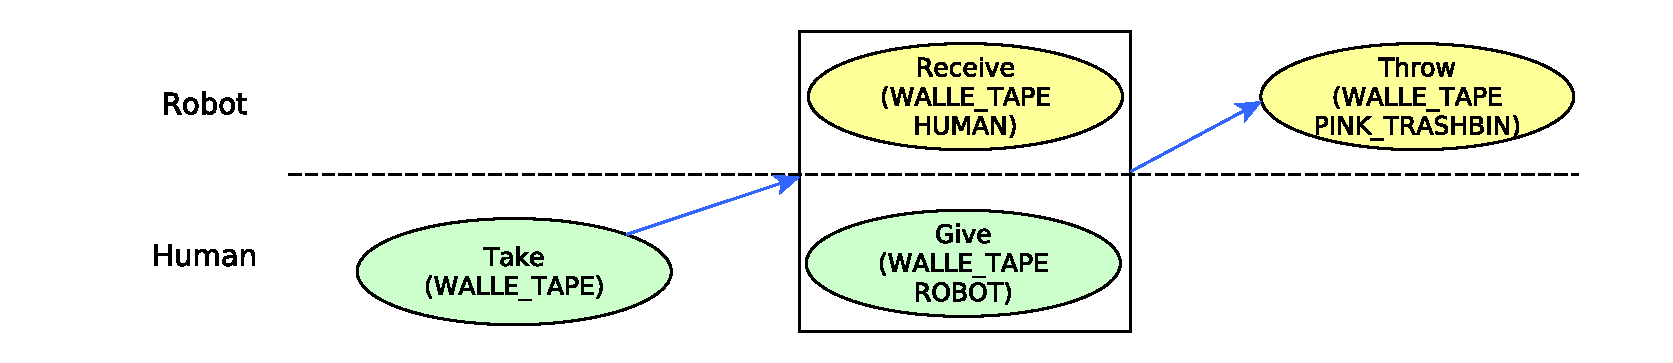
\includegraphics[scale=0.5]{img/case_study/helper/plan4.pdf}
      }
  \label{fig:case_study-helper-scenario3}
\end{figure}


After taking and throwing the $LOTR\_TAPE$, the robot tries to take the
$WALLE\_TAPE$, but fails because it is too far. The robot informs the user
and replans. The agents execute the plan, completing the task.

\item
\textbf{Replanning after human inactivity}.
In this run the robot computes that the $GREY\_TAPE$ and $PINK\_TRASHBIN$
are reachable only by the human, while the $WALLE\_TAPE$ is reachable only by the robot. The robot computes a plan
and starts executing it, observing the human reactions. 
 After an initial stage when the human is
commited to the task, he does not execute a part of the plan (taking
the final tape and throwing it), so the robot looks for another
plan. The only solution to the problem is the one already computed at
the beginning, so the robot decides to ask
 the human to take the tape and throw it. A run of this
scenario is shown in figure ~\ref{fig:case_study-helper-experiment}. 
\end{itemize}

 
\begin{figure}
  \caption{The picture shows a run of our 'replanning after human
    inactivity scenario'. The different
    rows show, starting from top to bottom: the real world picture,
    the world state representation built by the robot, symbolic facts
    input in the knowledge base at each time step, action taken by each
    agent at each time step, the current plan calculated by the robot.}
  \centering
  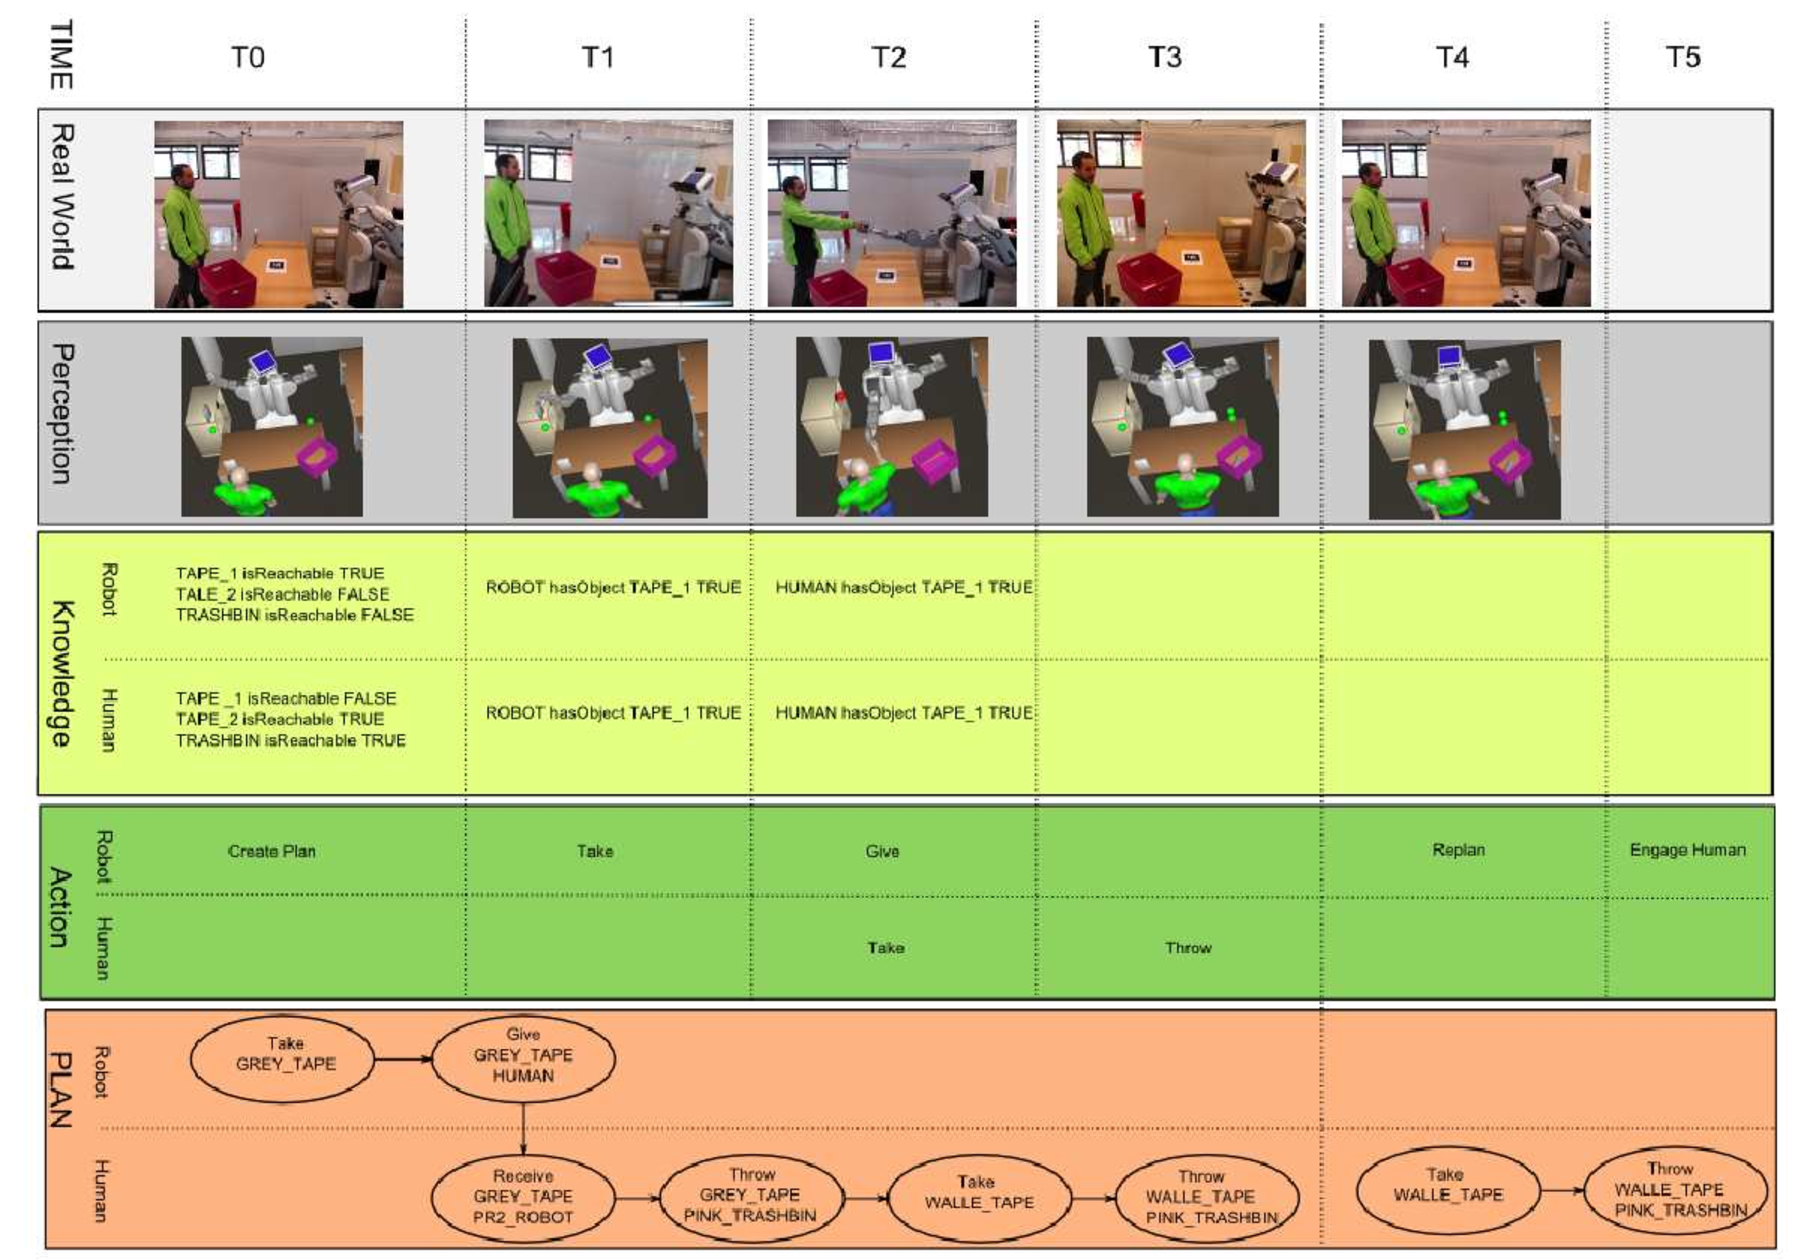
\includegraphics[angle=90, scale=0.7]{img/case_study/helper/plan.pdf}
  \label{fig:case_study-helper-experiment}

\end {figure}


\subsection{Discussion}
We review some of the main results of our experiments in this scenario:
\begin{itemize}

\item
\textbf{The system is able to handle joint goals}.
The system is able to create shared plans with different users, taking
into account the capabilities of each agent. When unexpected changes
in the world or task status arise, the system is able to quickly
replan, adapting to new scenarios. The system is able to execute this
joint goal in a human aware way. 
                                
\item
\textbf{The system is able to handle joint actions}.
The system is able to estimate user intentions in collaborative tasks and to choose appropriate actions, using a set of POMDP models.

\item
\textbf{The system is able to handle user preferences}.
The system is able to adapt itself to user preferences, allowing the
human partner to give commands or to be more passive in its role and
switching from one modality to the other. 
\item
\textbf{The system is able to handle each agent beliefs}.
The system is able to represent different belief states for different agents and to take into accout what users can see, reach and know when creating a plan.

\item
\textbf{The system is able to monitor human actions}.
The system was able to understand when the human performed action such as taking or throwing objects.
\end{itemize}



%\bibliographystyle{plainnat} % Use the "unsrtnat" BibTeX style for formatting the Bibliography
%\bibliographystyle{apalike}
%\bibliographystyle{unsrtnat}
\bibliographystyle{IEEEtran}

\lhead{\emph{Bibliography}} % Change the page header to say "Bibliography"
\bibliography{all.bib} % The references (bibliography) information are stored in the file named "thesis.bib"

\newpage
\appendix
\end{document}  